%\documentclass[smalldemyvopaper,11pt,twoside,onecolumn,openright,extrafontsizes]{memoir}
\documentclass[20pt,oneside,openright,extrafontsizes,landscape,a5paper]{memoir}
\usepackage{yfonts,color,hyperref}
\def\initdefault{yinit}
  \usepackage{fontspec}
%\usepackage[T1]{inputenc}
\usepackage{fontspec}
\usepackage[spanish]{babel}
\usepackage{xsavebox} %save content for repeated use
\usepackage{atbegshi} %insert material on every page
\usepackage[x11names,dvipsnames]{xcolor} 
\usepackage{wrapfig}  
\usepackage{tikz}
\usepackage[tmargin=1.cm,bmargin=1cm,lmargin=2cm,rmargin=1cm]{geometry}
%\usepackage[margin=1cm]{geometry}% for screen preview
\usepackage{graphicx}
\setmainfont{juan_letra_reg}
%\DeclareFontFamily{LYG}{OldNewspaperTypes}{}
	
%\AtBeginShipout{
%	\AtBeginShipoutUpperLeft{\raisebox{-\height}{\xusebox{PageBGPicture}}}
%}
\tolerance=1
\emergencystretch=\maxdimen
\hyphenpenalty=10000
\hbadness=10000
\usetikzlibrary{calc}
\usepackage{relsize}
\tikzset{fontscale/.style = {font=\relsize{#1}}
}
\setlength\parindent{0pt}

\begin{document}
%\begin{normal}

\pagenumbering{gobble}
\noindent
		\begin{tikzpicture}[remember picture, overlay]
			\node [inner sep=0pt, minimum width=\paperwidth, minimum height=\paperheight] at (current page.center) {\includegraphics[width=\paperwidth,height=\paperheight,angle=0]{portada}};
		\end{tikzpicture}
%\iffalse

\newpage
		\begin{tikzpicture}[remember picture, overlay]
	\node [inner sep=0pt, minimum width=\paperwidth, minimum height=\paperheight] at (current page.center) {\includegraphics[width=\paperwidth,height=\paperheight,angle=0]{presenta}};
\end{tikzpicture}
%\end{normal}
%\begin{minipage}{.35\textwidth}

HOLA, MI NOMBRE ES OTTOKO, VIVO EN VILLA DEVOTO. 

SI BIEN PUEDE PARECERLES QUE LLEVO UNA VIDA 

APACIBLE Y HASTA UN TANTO PEREZOSA, 

VOY A 

CONTARLES 

LA ÚLTIMA 

DE MIS 

INTRÉPIDAS

 AVENTURAS.	
		

%\end{minipage}	

\newpage
\begin{tikzpicture}[remember picture, overlay]
	\node [inner sep=0pt, minimum width=\paperwidth, minimum height=\paperheight] at (current page.center) {\includegraphics[width=\paperwidth,height=\paperheight,angle=0]{presenta2}};
	
	\node[text width=\textwidth,xshift=0cm,yshift=0cm] at (current page.center){PUEDE QUE ALGUIEN DESCONFÍE DE LOS RELATOS DE UN GATO NEGRO, $\ldots$ ¿QUIÉN NO HA ESCUCHADO DECIR QUE LOS GATOS NEGROS TRAEMOS MALA SUERTE? ¡PURAS PATRAÑAS! 
	
A VECES, REPETIR COSAS SIN PENSAR 

RESULTA 	
	FÁCIL Y CÓMODO. POR ESO, AÚN
	
	 HOY HAY 	
	 PERSONAS QUE CREEN QUE EL 
	 
	 PLANETA 	 
	 TIERRA	 
	  ES PLANO, QUE LA 
	  
	  ASTROLOGÍA	  
	   SIRVE	  
	   PARA   
	  CONOCERSE,
	  
	   QUE EXISTEN
	  	   EL MAL	  
	   DE OJO 	  
	  Y LAS BRUJERÍAS$\ldots$ LOS HUMANOS 
	  
	  	SON CAPACES DE ÉSTAS

	 Y TANTAS OTRAS SANDECES CUANDO NO TIENEN GANAS DE RAZONAR. 
		
	};
	

\end{tikzpicture}
\newpage
\begin{tikzpicture}[remember picture, overlay]
	\node [inner sep=0pt, minimum width=\paperwidth, minimum height=\paperheight] at (current page.center) {\includegraphics[width=\paperwidth,height=\paperheight,angle=0]{paloma1}};
\node[text width=3.5cm,yshift=4.75cm,xshift=.45\textwidth] at (current page.center){¡UH! ¡UH! ¡UH!};
\end{tikzpicture}	
				A MÍ ME GUSTA PENSAR.
				
				 DE OTRA FORMA SERÍA DIFÍCILMENTE UN 
				 
				 BUEN CAZADOR FELINO. SEPAN QUE YA				
				
			 DESDE CHIQUITO, ME INTERESABA 
			 
			 REFLEXIONAR 			 
			 SOBRE CÓMO ATRAPAR 
			 
			 PALOMAS.
			
			¡PALOMAS! ALGUNOS CAMARADAS LAS 
						LLAMAN 			
			
			 RATAS DEL AIRE.   
			  ¡PERO SÍ!, LOS 
			  			  GATOS 
			  			  
	  		SABEMOS QUE  			 
			 EXISTEN LOS			 
			  MURCIÉLAGOS
			  
			   SIN EMBARGO, HAY MUCHOS MENOS  	DE ELLOS 
			 	 	 
			 QUE  PALOMAS EN LAS CIUDADES. ESTAS AVES			
						
			ADAPTARON SU PLUMAJE  AL COLOR 	DEL CEMENTO 
			
			DE LOS EDIFICIOS,  DEL ASFALTO, DE LAS CALLES, 
			
			AUNQUE, PARA MÍ, IMITAN MÁS BIEN AL TINTE DE LA MUGRE.	

\newpage
\begin{tikzpicture}[remember picture, overlay]
	\node [inner sep=0pt, minimum width=\paperwidth, minimum height=\paperheight] at (current page.center) {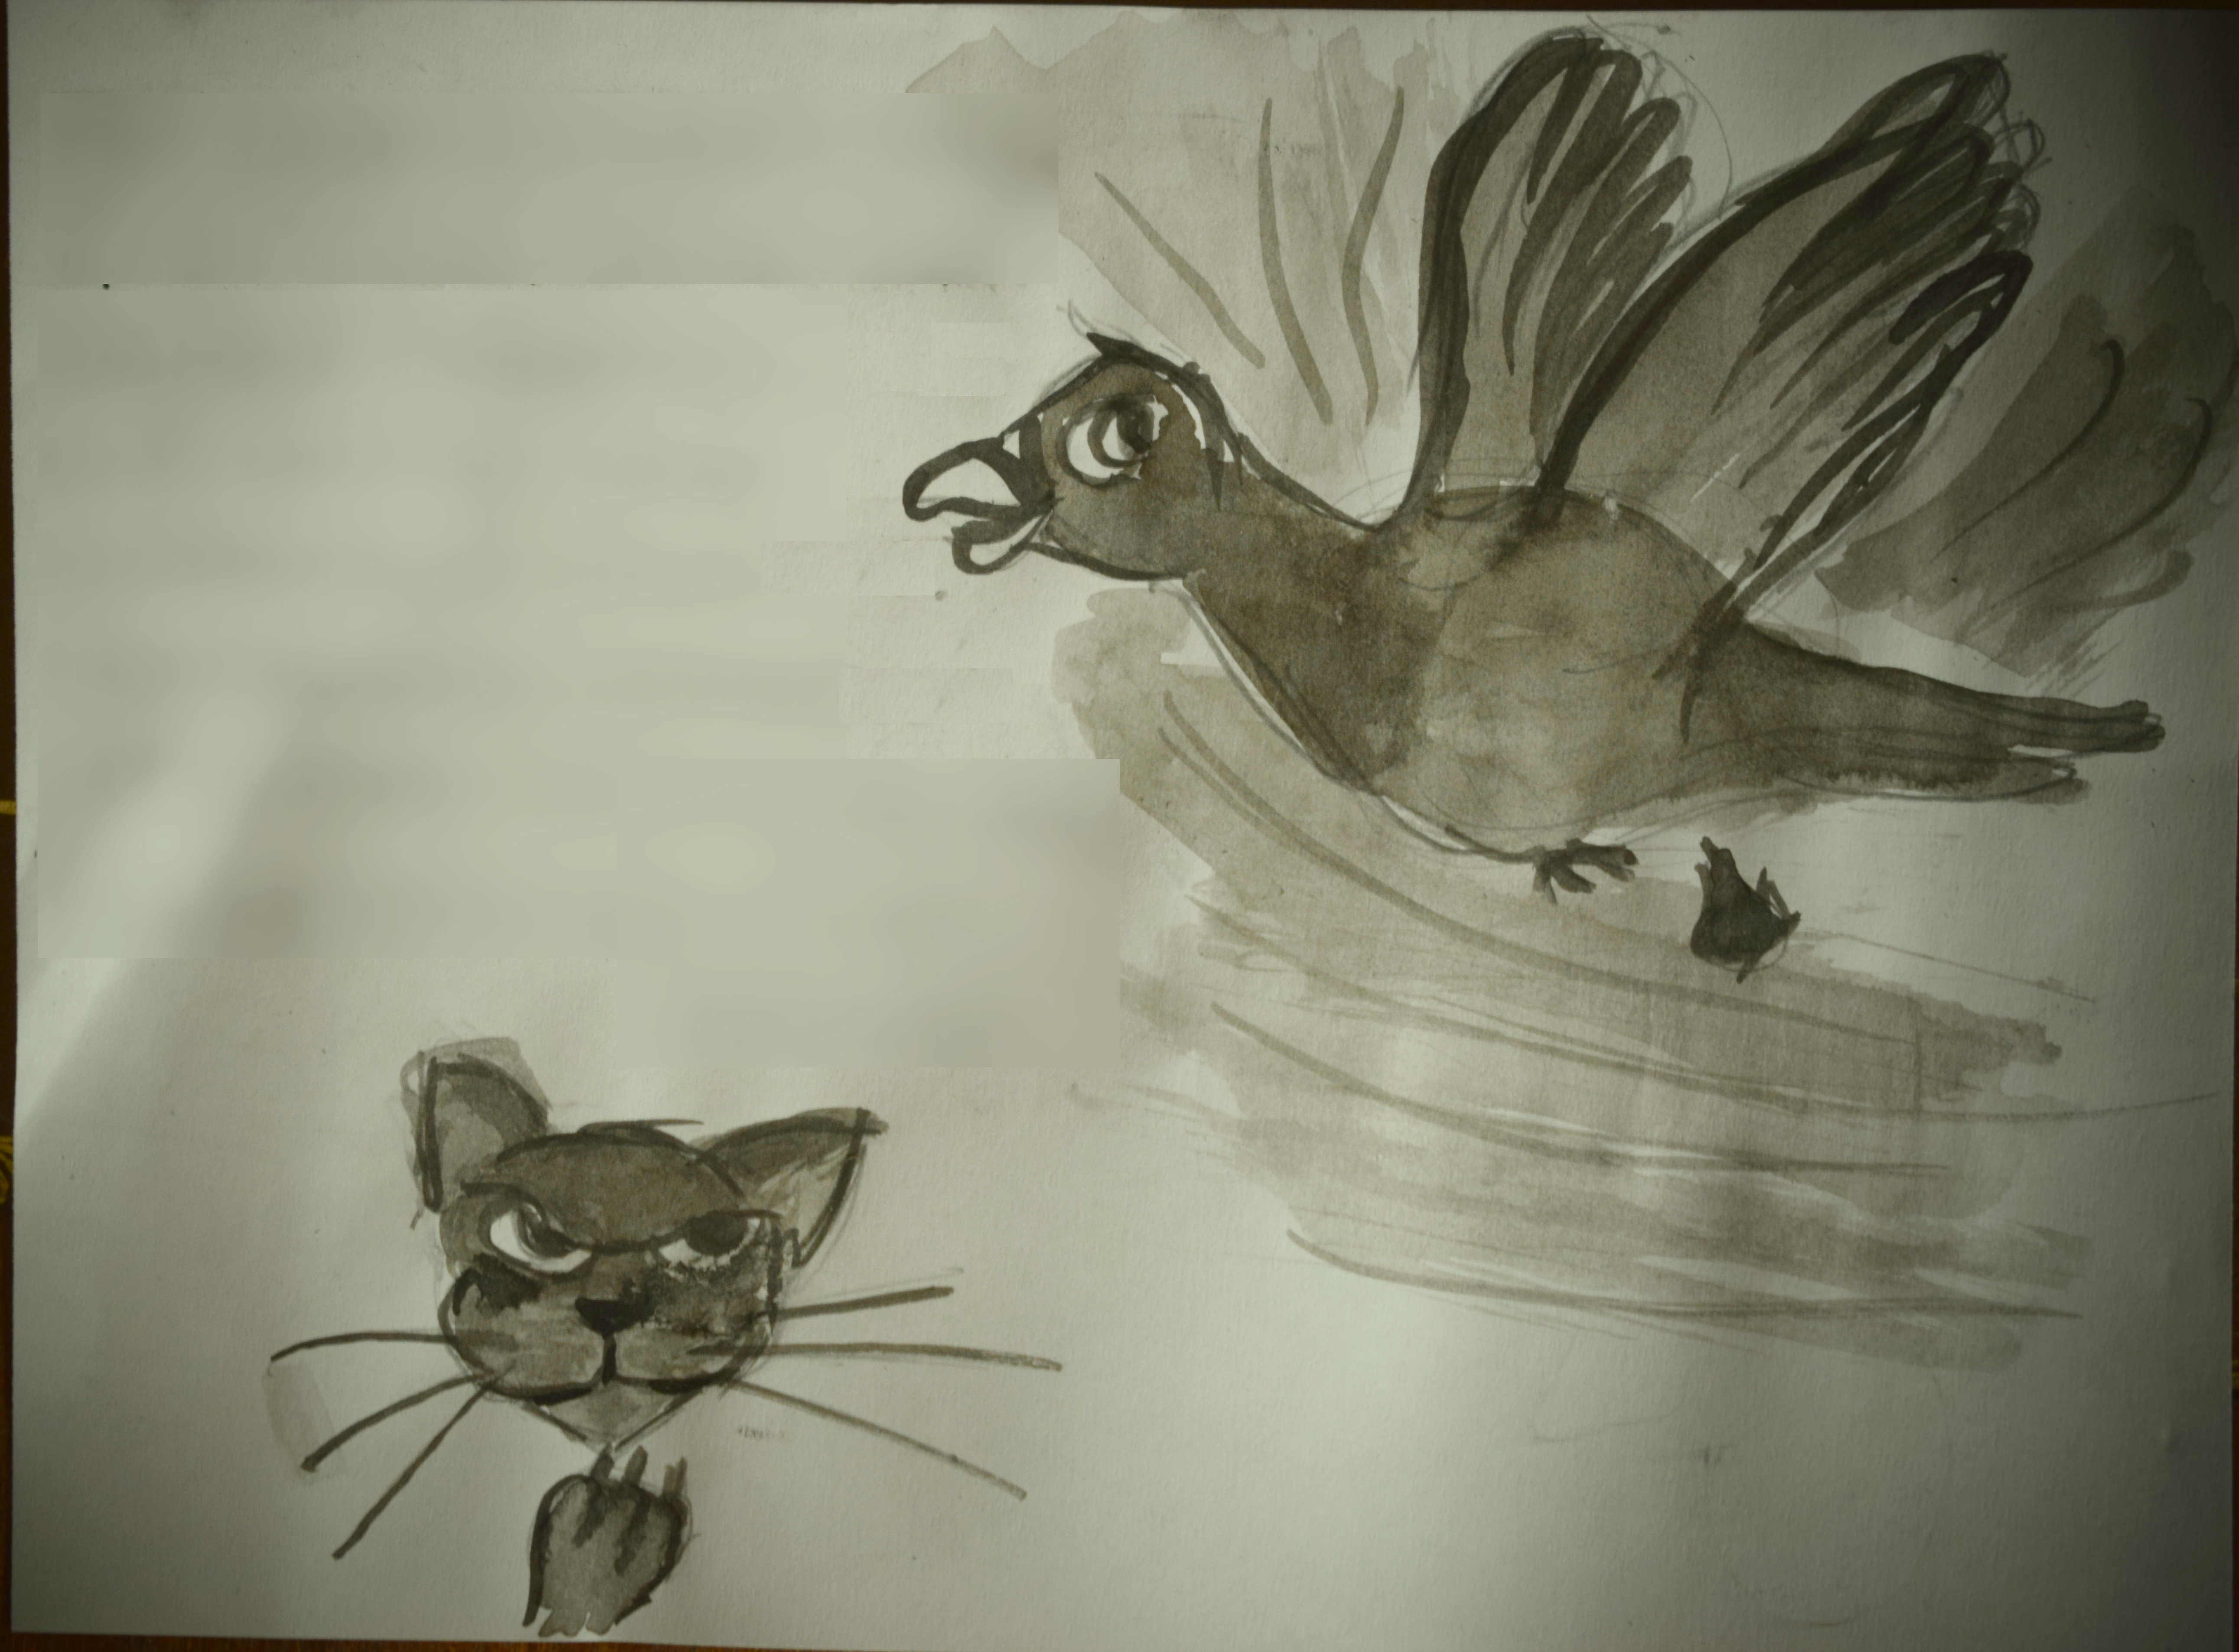
\includegraphics[width=\paperwidth,height=\paperheight,angle=0]{paloma2}};
\end{tikzpicture}
SI BIEN DE MIRADA TORPE 

Y DE CAMINAR MUY POCO ELEGANTE, 
			\newline\newline\newline
			
			RECONOZCO QUE SON MUY ASTUTAS
			
			 PARA EMPRENDER EL VUELO.
				\newline\newline
			\begin{flushright}
				\begin{minipage}[r]{.5\textwidth}
	TAMBIÉN ADMIRO ALGUNA DE SUS HABILIDADES MUY PRÁCTICAS PARA LA VIDA COTIDIANA, ¡ Y SIN PIEDRITAS!
\end{minipage}
			\end{flushright}	

	
	
	
	


\newpage
\begin{tikzpicture}[remember picture, overlay]
	\node [inner sep=0pt, minimum width=\paperwidth, minimum height=\paperheight,opacity=0.9] at (current page.center) {\includegraphics[width=\paperwidth,height=\paperheight,angle=0]{comiendo}};
\end{tikzpicture}	
	PUES ME ENCONTRABA MUY TRANQUILO UNA MAÑANA COMIENDO MIS DELICIOSAS CROQUETAS PARA GATO (A VECES CONFIESO QUE ME HE DESAYUNADO CUCARACHAS PERO ESA ES OTRA HISTORIA) 
			\newline\newline\newline
						\newline\newline\newline	\newline\newline 
			CUANDO ESCUCHÉ DESDE EL PATIO EL ARRULLO DE UNAS PALOMAS.
			ESTABA ABIERTO EL VENTANAL Y DECIDÍ DAR UN VISTAZO . ALLÍ ESTABAN, CHARLANDO ENTRE ELLAS. CON MI HABITUAL CURIOSIDAD FELINA, ME ACERQUÉ UN POCO HACIA DONDE ESTABAN.
		
	
		
	
	

\newpage
\begin{tikzpicture}[remember picture, overlay]
	\node [inner sep=0pt, minimum width=\paperwidth, minimum height=\paperheight] at (current page.center) {\includegraphics[width=\paperwidth,height=\paperheight,angle=0]{salto_paloma}};
\end{tikzpicture}	
				CASI AL INSTANTE \hspace{.3\textwidth}¡VI QUE ME HABÍAN ENGAÑADO! 
				
				PUES UNA AVE \hspace{.3\textwidth}INSOLENTE, HABÍA APROVECHADO 
				
				MI DISTRACCIÓN 
				
				PARA SAQUEAR 				
				MI PLATO.
				
				REACCIONÉ.
				
			SI BIEN FUE UNO			
			 DE MIS MEJORES		
			 	 
			  SALTOS, NO CONSEGUÍ 			  
			  ATRAPARLA. ¡UN GATO 
			  
			  JOVEN COMO YO TENDRÍA MÁS
			  
			   OPORTUNIDADES EN EL FUTURO! 
			  
			  DESDE LO ALTO DEL MURO, LAS 			  
			  PALOMAS SE
			  
			   BURLABAN DESCARADAMENTE. 
			  
			  SÍ, O AL MENOS ESO PENSÉ DE LOS MÚLTIPLES 
			  
			  'UH-UH-UH' QUE LLEGABAN A MIS OÍDOS.
			  
			   ALGO FURIOSO, DECIDÍ DARLES UNA LECCIÓN DE HUMILDAD.

		
	

%
%\newpage
%\begin{tikzpicture}[remember picture, overlay]
%	\node [inner sep=0pt, minimum width=\paperwidth, minimum height=\paperheight] at (current page.center) {\includegraphics[width=\paperwidth,height=\paperheight,angle=0]{salto_paloma}};
%	
%		\node[text width=14cm,xshift=-4cm,yshift=0cm] at (current page.center){SI BIEN FUE UNO
%			
%			DE MIS MEJORES
%			
%			SALTOS, NO CONSEGUÍ 
%			
%			ATRAPARLA. ¡UN GATO JOVEN COMO YO TENDRÍA MÁS OPORTUNIDADES EN EL FUTURO! 
%			
%			DESDE LO ALTO DEL MURO, LAS 
%			
%			PALOMAS SE BURLABAN DESCARADAMENTE. 
%			
%			SÍ, O AL MENOS ESO PENSÉ DE LOS MÚLTIPLES 'UH-UH-UH' QUE LLEGABAN A MIS OÍDOS. ALGO FURIOSO, DECIDÍ DARLES UNA LECCIÓN DE HUMILDAD.
%		};	
		
	
	
%\end{tikzpicture}

\newpage
\begin{tikzpicture}[remember picture, overlay]
	\node [inner sep=0pt, minimum width=\paperwidth, minimum height=\paperheight] at (current page.center) {\includegraphics[width=\paperwidth,height=\paperheight,angle=0]{reflexion}};
\end{tikzpicture}
TOMÉ CORAJE Y SEGUÍ TREPANDO. UTILICÉ LA ESQUINA 
			
			QUE FORMAN LAS PAREDES  
			
			Y FINALMENTE ALCANCÉ
			
			 TODO LO ALTO 		DEL MURO.
			 
			  HAY ALLÍ UNA 		ESPECIE 
			  
			  DE CANTERO Y ME
			
			 METÍ DENTRO DE LO QUE
			 
			 ES  UNA CANALETA. ES DONDE
			 
			  CORRE  			 EL AGUA QUE MIRO CAER
			  
			   FASCINADO   LOS DÍAS DE LLUVIA.
			   
			    DESDE ESE LUGAR  PODÍA VER TODO EL 
			    
			    PATIO DONDE SOLEMOS JUGAR. MI ESFUERZO RESULTÓ TAN GRANDE QUE NECESITÉ DESCANSAR UN RATO.

	
	


\newpage
\begin{tikzpicture}[remember picture, overlay]
	
	\node [inner sep=0pt, minimum width=\paperwidth, minimum height=\paperheight] at (current page.center) {\includegraphics[width=\paperwidth,height=\paperheight,angle=0]{paper2}};
			\end{tikzpicture}

			A LOS GATOS NOS GUSTAN LAS SIESTAS EN LAS ALTURAS Y AL CALOR DEL SOL, SOBRE TODO EN INVIERNO.
			
			YA ME HABÍA OLVIDADO DE LAS PALOMAS, HABÍAN VOLADO Y VIENDO UN GATO NEGRO EN LO ALTO DE UN MURO BLANCO, DUDO QUE VOLVERÍAN POR MI CASA POR UN BUEN RATO.
			
			CUANDO ME LEVANTÉ, EXPLORÉ LOS ALREDEDORES PASEANDO POR EL CANTERO. SABÍA QUE AL LADO VIVÍAN DOS PERRITOS BASTANTE CARGOSOS, POR COMO SOLÍAN LADRAR. Y AL FIN LAS VEÍA! ERAN UNA PERRA LABRADOR NEGRA Y UNA CANICHE BLANCA. PASEABAN SIN CORREA, SEGUIDAS POR UN VIEJO DE CAMINAR TORPE Y DESCUIDADO. LAS PERRITAS SE PUSIERON A HACER SUS COSAS  EN LA VEREDA Y EL SEÑOR NI AMAGÓ PARA LIMPIARLA.
		
		
\end{document}
 
\newpage
\begin{tikzpicture}[remember picture, overlay]
	
		\node [inner sep=0pt, minimum width=\paperwidth, minimum height=\paperheight] at (current page.center) {\includegraphics[width=\paperwidth,height=\paperheight,angle=0]{paper2}};
\node[xshift=.35\textwidth] at (current page.center){\includegraphics[width=.5\textwidth,trim=1.9cm 2cm 1.5cm 1.6cm,clip]{arbol_tilo}};
\end{tikzpicture}
		ESPERÉ UN RATO, NO PODRÍA BAJAR CON 
		
		ESAS DOS PERRITAS 	SUELTAS. Y PARA PODER 
		
		DESCENDER, 		NECESITABA ALGO ENTRE 
		
		EL		
		ALTO MURO Y EL PISO. 
		
		PENSÉ EN LOS ÁRBOLES DE TILO QUE 
		
		ESTÁN 		JUNTO A LA CASA. 		SON MUY 
		
		LINDOS, DE COPAS REPLETAS DE HOJAS EN 
		
		PRIMAVERA, Y  QUE CAEN, JUNTO A SEMILLAS 
		
		DURANTE EL OTOÑO. MUCHAS DE ELLAS TERMINAN
		
		 EN NUESTRO PATIO Y SON BUENOS JUGUETES.
		 
		  PERO SUFICIENTE CON LOS JUEGOS. 
		SIEMPRE ME
		
		 DICEN QUE PAREZCO UNA PEQUEÑA PANTERA 
		NEGRA$\ldots$ 
		
		ERA HORA DE DEMOSTRARLO. 
	
	


 

\newpage
 \begin{tikzpicture}[remember picture, overlay]
 	
 		\node [inner sep=0pt, minimum width=\paperwidth, minimum height=\paperheight] at (current page.center) {\includegraphics[width=\paperwidth,height=\paperheight,angle=0]{paper3}};
  \end{tikzpicture}	
 			DURANTE MI SIESTA YA HABÍA PENSADO EN EL SALTO. A MENUDO PIENSO EN MIS PROEZAS FELINAS A LA HORA DE DORMIR, ASÍ ME DUERMO CON UNA SONRISA.
 			
	PERO AHORA, BIEN DESPIERTO, NO IBA A FALLAR NINGÚN CÁLCULO. TODO MI ENTRENAMIENTO EN EL PATIO, TREPANDO EN LA BIBLIOTECA, SOBRE EL PIANO, SOBRE LA SILLA ALTA$\ldots$ TODO IBA A SERVIRME EN MI CAÍDA CON ESTILO SOBRE LA RAMA DEL ÁRBOL DE TILO.  



\newpage
\begin{tikzpicture}[remember picture, overlay]
	
	\node [inner sep=0pt, minimum width=\paperwidth, minimum height=\paperheight] at (current page.center) {\includegraphics[width=\paperwidth,height=\paperheight,angle=0]{paper3}};
	\node[xshift=0cm,yshift=4cm] at (current page.center){\includegraphics[width=.8\textwidth,trim=1.9cm 2cm 1.5cm 1.6cm,clip]{arriba_arbol}};
\end{tikzpicture}

 \vspace{.7\textheight}
	 Y ASÍ FUE, UNA MANIOBRA LIMPIA Y DISTINGUIDA, SÉ QUIENES ESTARÍAN ORGULLOSOS DE MÍ. 
	
	



 \newpage
 \begin{tikzpicture}[remember picture, overlay]
 	
 		\node [inner sep=0pt, minimum width=\paperwidth, minimum height=\paperheight] at (current page.center) {\includegraphics[width=\paperwidth,height=\paperheight,angle=0]{paper3}};
  \end{tikzpicture}	
% 		\node[xshift=7cm,yshift=3cm] at (current page.center){\includegraphics[width=.4\textwidth,trim=1cm 0cm 1.cm 0cm,clip]{vereda1}};
% 		\node[text width=24cm,yshift=0cm] at (current page.center){
 			YA CAMINANDO POR LA VEREDA, DESDE AFUERA, LA CASA SE VEÍA
 MÁS GRANDE. VI ACERCARSE UN PERRO Y VOLVÍ A TREPARME AL ÁRBOL SIN PROBLEMAS.
 
 
\begin{wrapfigure}{r}{.45\textwidth}
\includegraphics[width=.4\textwidth,trim=1cm 0cm 1.cm 0cm,clip]{vereda1}
\end{wrapfigure}
AHORA QUE ME HABÍA OLVIDADO  DE 

LAS PALOMAS, DI UNA VUELTA A LA PEQUEÑA MANZANA QUE CONTIENE A MI CASA. YA HABÍA VISTO UN POCO LA CALLE CUANDO  ME HABÍAN LLEVADO A VACUNAR.  
PERO, ¿QUÉ DIRECCIÓN TOMAR? DECIDÍ IR HACIA DONDE VIERA PERSONAS.


 \newpage
\begin{tikzpicture}[remember picture, overlay]
 		\node [inner sep=0pt, minimum width=\paperwidth, minimum height=\paperheight] at (current page.center) {\includegraphics[width=\paperwidth,height=\paperheight,angle=0]{paper4}};
\end{tikzpicture}	
 PUES PODÍA SER INTERESANTE APRENDER ALGO NUEVO. FUI AVANZANDO DE POCO ESCONDIÉNDOME PRIMERO EN UN CANTERO, LUEGO DETRÁS DE UNAS PALMERAS.
 
	IBA A TENER QUE CRUZAR LA CALLE. ES UNA SENSACIÓN DISTINTA,  PUES  LA SUPERFICIE NO ES LA MISMA QUE LA VEREDA Y HAY UNA BAJADITA, QUE LLAMAN CORDÓN.
 
A MENUDO, HAY ASFALTO, QUE ES UNA SUPERFICIE LISA Y UN POCO RUGOSA A LA VEZ. 
 	  
 	  
LOS ADOQUINES, EN CAMBIO, SON COMO PIEDRAS TODAS DEL MISMO TAMAÑO, ORDENADAS REGULARMENTE. SE VEN MUY DUROS Y LISOS, AUNQUE LOS AUTOS CUANDO PASAN HACEN MUCHO RUIDO PORQUE LES DAN COMO GOLPECITOS.  	  
 	  
 	  
 	  EN OCASIONES, SE CONSERVAN DESDE LA ÉPOCA DE CUANDO MI PAPÁ ERA CHIQUITO.
%};
 	

 \newpage
\begin{tikzpicture}[remember picture, overlay]
		\node [inner sep=0pt, minimum width=\paperwidth, minimum height=\paperheight] at (current page.center) {\includegraphics[width=\paperwidth,height=\paperheight,angle=0]{paper4}};
	\end{tikzpicture}
	\begin{wrapfigure}{r}{.4\textwidth}
 \includegraphics[width=.4\textwidth,trim=1cm 0cm 1.cm 0cm,clip]{rueda_auto}
	\end{wrapfigure}
	ANTES DE IR SOBRE LA CALLE, ME DETUVE UNOS INSTANTES AL COSTADO DE UNA RUEDA DE AUTO.
	ATRAVESÉ LA CALLE DE ADOQUINES MIRANDO BIEN QUE NO HUBIERA NINGÚN AUTO EN MOVIMIENTO.  NI BIEN LLEGUÉ A LA OTRA VEREDA, PERCIBÍ UN AROMA DELICIOSO. YA LO HABÍA SENTIDO ANTES,	 HACE UNOS MESES, CREO QUE 
	SE TRATABA DE COMIDA CHINA: CHAW FAN Y BUÑUELOS DE POLLO!

\newpage

\begin{tikzpicture}[remember picture, overlay]

		\node [inner sep=0pt, minimum width=\paperwidth, minimum height=\paperheight] at (current page.center) {\includegraphics[width=\paperwidth,height=\paperheight,angle=0]{paper5}};
	\end{tikzpicture}
\begin{wrapfigure}{r}{.53\textwidth}
	\includegraphics[width=.5\textwidth,trim=0cm 0cm 0.cm 0cm,clip]{comida_china}
\end{wrapfigure}
			PERO NO VEÍA NADA MÁS QUE UNA PERSIANA DE METAL BAJA Y AL LADO UNA PUERTA CERRADA. AGUCÉ MI OÍDO FELINO Y ESCUCHÉ MOVIMIENTO DE PERSONAS AL INTERIOR.  DE PRONTO, 
			SENTÍ UN AUTO ACERCARSE Y ME DÍ VUELTA. SE TRATABA DE UN AUTO CON LUCES PARPADEANTES AZULES Y SE DETUVO
		JUSTO A METROS DE DONDE YO ESTABA. DE UN SALTO ME PUSE A UNA BUENA DISTANCIA A OBSERVAR. 
		DESCENDIÓ UN SEÑOR QUE VESTÍA UN UNIFORME AZUL OSCURO, Y RÁPIDAMENTE SE ACERCÓ A LA PERSIANA.


\newpage

\begin{tikzpicture}[remember picture, overlay] 
		
	\node [inner sep=0pt, minimum width=\paperwidth, minimum height=\paperheight] at (current page.center) {\includegraphics[width=\paperwidth,height=\paperheight,angle=0]{paper6}};
\end{tikzpicture}

 
		EL UNIFORMADO GOLPEÓ RÁPIDO TRES VECES CON LA MITAD DE SU DEDO ÍNDICE  EN LA PERSIANA.
		DE PRONTO, UNA PEQUEÑA PUERTA SE ABRIÓ Y UN BRAZO ASOMÓ CON	  LO QUE IMAGINÉ ERA UN
		\begin{wrapfigure}{r}{.5\textwidth}
			\includegraphics[width=.45\textwidth,trim=0cm 0cm 0.cm 0cm,clip]{frente_al_chino}
		\end{wrapfigure}     
    BANQUETE FENOMENAL DE COMIDA CHINA. POR UN INSTANTE, MEDÍ LAS POSIBILIDADES DE ROBAR GRACIAS A MIS PODEROSOS RECURSOS FELINOS. MÁS DE UNA VEZ HABÍA CONSEGUIDO EN CASA PEDACITOS DE JAMÓN, DE QUESO, DE PIZZA, DE POLLO, BUENO, ¡Y ALGUNA COSA MÁS DE LA QUE AÚN NO SE DIERON CUENTA! 








\newpage

\begin{tikzpicture}[remember picture, overlay]
	
		\node [inner sep=0pt, minimum width=\paperwidth, minimum height=\paperheight] at (current page.center) {\includegraphics[width=\paperwidth,height=\paperheight,angle=0]{paper7}};
\end{tikzpicture}
	\begin{wrapfigure}{r}{.35\textwidth}
		\includegraphics[width=.27\textwidth,trim=0cm 0cm 0cm 0cm,clip]{uñas}
	\end{wrapfigure}
		SEGUÍA LOS MOVIMIENTOS EN TORNO A LA COMIDA CUANDO MIS SENTIDOS
		
		GATUNOS ME INDICARON QUE OTRO HUMANO SE ACERCABA.

		MIRÉ CON EL COSTADO DE MIS OJOS Y ALCANCÉ A DETECTAR UNA SEÑORA DE VOZ 
		ALGO ESTRIDENTE ¡QUE PARECÍA QUE ME HABLABA A MÍ!

%		\node[text width=15cm,xshift=-4cm] at (current page.center){
		-AY, ¡PERO MIRÁ ESTE NEGRITO 
		
		TODO BONITO!

		VI ACERCARSE UNA GARRA HUMANA. 
		
		¡NUNCA HABÍA VISTO NADA SEMEJANTE!


%};
	

\newpage
\begin{tikzpicture}[remember picture, overlay]
	\node [inner sep=0pt, minimum width=\paperwidth, minimum height=\paperheight] at (current page.center) {\includegraphics[width=\paperwidth,height=\paperheight,angle=0]{uñas2}};
\end{tikzpicture}			
			ME ARQUEÉ TODO DEL SUSTO, CON LOS PELOS ERIZADOS, PARA AVISAR QUE YO IBA A USAR LAS MÍAS.		
			PERO LA SEÑORA QUE TENÍA LAS GARRAS, SONREÍA Y NO PARECÍA QUERER ATACARME.
			
			-ESTÁ SOLITO, ¡MIRALO! ¿SE HABRÁ PERDIDO?
			\newline
			\vspace{.35\textheight}
			- ¡MAMÁ, DEJALO, ¿NO VES QUE ES MEDIO SALVAJE?
		
	UNA NIÑA ACOMPAÑABA A LA DAMA DE GARRAS AZULES.		
	 PARECÍA ENTENDER MEJOR A LOS FELINOS.
		
		- ¡AY, BUENO! ¡QUÉ CARÁCTER! 
		
		POR LAS DUDAS, ME FUI PRUDENTE PARA NO TENER PROBLEMAS.
\newpage
\begin{tikzpicture}[remember picture, overlay]
	\node [inner sep=0pt, minimum width=\paperwidth, minimum height=\paperheight] at (current page.center) {\includegraphics[width=\paperwidth,height=\paperheight,angle=0]{paper8}};
	\node [inner sep=0pt, minimum width=\paperwidth] at (current page.center) {\includegraphics[width=\paperwidth,angle=0]{uñas3}};
	
\end{tikzpicture}	
		SEGUÍ MI CAMINO HASTA LLEGAR A UN MUY CURIOSO LOCAL. 
		
\begin{flushright}
	\begin{minipage}{.5\textwidth}
ASÍ PUDE DESCUBRIR DONDE LAS PERSONAS PODÍAN TALLARSE
ESAS GARRAS TAN RARAS Y DE COLORES. 			
A MI ME GUSTAN MIS GARRITAS NEGRAS.	
	\end{minipage}
\end{flushright}
	
		
		


\newpage
\begin{tikzpicture}[remember picture, overlay]
	\node [inner sep=0pt, minimum width=\paperwidth, minimum height=\paperheight] at (current page.center) {\includegraphics[width=\paperwidth,height=\paperheight,angle=0]{paper9}};
\node [inner sep=0pt,  minimum height=\paperheight,xshift=4cm] at (current page.center) {\includegraphics[height=\paperheight,angle=0]{mexicano1}};
	
\end{tikzpicture}	
 \begin{minipage}{.5\textwidth}
ALGO MUCHO MÁS INTERESANTE SE HALLABA JUSTO
 UNOS
 
  METROS
    MÁS ADELANTE. 
    
    ESQUELETOS HUMANOS 
    
    VESTIDOS SIMPÁTICAMENTE 
    
    DECORABAN LA ENTRADA A 
    
    UN RESTAURANTE.

LLEGABA UN MUY 
AGRADABLE 

AROMA A COMIDA, 

NADA QUE PUDIERA DAÑAR A UNA BUENA DIETA FELINA.



¡ES HERMOSO! ME PROMETÍ VENIR A CENAR ALGÚN DÍA QUE PUDIERA FESTEJAR ALGO. ¡ÓRALE JUANITO!
 \end{minipage}

 
		



\newpage
\begin{tikzpicture}[remember picture, overlay]
	\node [inner sep=0pt, minimum width=\paperwidth, minimum height=\paperheight] at (current page.center) {\includegraphics[width=\paperwidth,height=\paperheight,angle=0]{reflexion2}};
\end{tikzpicture}	
\begin{minipage}{.6\textwidth}	
		USTEDES SE PREGUNTARÁN COMO 
		
		CONOZCO TANTO DE GASTRONOMÍA,
		
		 PUES YA 		
		COMENTÉ QUE EL CHAW 
		
		FAN 
		Y LOS 		
		BUÑUELOS DE POLLO
				 SON 
				 
				 MUY 		
				 		BUENOS,				
		Y AHORA PENSANDO 
		
		EN COMER 
		ALGÚN 		
		BURRITO 		
		MEXICANO$\ldots$ 
		
		PUES DEBO 
				CONFESAR 	
		 QUE MÁS DE
		 
		  UNA VEZ, 
		 A ESCONDIDAS,	 
		  HE PROBADO 
		  
		  DIFERENTES 
		  		  PLATOS EN 		  
		  CASA. 		  
		  HACE 
		  
		  NO MUCHO TIEMPO ATRÁS, 
		  		  ROBÉ UN 
		  
		  BUEN PEDAZO
		  		   DE PIZZA CON JAMÓN. 
		   
		   ¡RECIÉN SE DIERON CUENTA AL		   
		    DÍA SIGUIENTE! 
		    
		    JEJEJE.
 \end{minipage}



\newpage
\begin{tikzpicture}[remember picture, overlay]
	\node [inner sep=0pt, minimum width=\paperwidth, minimum height=\paperheight,xshift=5cm] at (current page.center) {\includegraphics[ height=\paperheight,angle=0]{biblio}};
	\end{tikzpicture}

\begin{minipage}{.4\textwidth}	\vspace{.3\textheight}
		OTTOKO LES RECUERDA QUE PARA ESCRIBIR HISTORIAS, HACE BIEN LEER BUENAS HISTORIAS. POR ESO SIEMPRE PASEA POR LA BIBLIOTECA!! 
 \end{minipage}

\newpage
\begin{tikzpicture}[remember picture, overlay]
	\node [inner sep=0pt, minimum width=\paperwidth, minimum height=\paperheight] at (current page.center) {\includegraphics[width=\paperwidth,height=\paperheight,angle=0]{paper10}};
	\node [inner sep=0pt,  minimum height=\paperheight,xshift=7cm] at (current page.center) {\includegraphics[height=\paperheight,angle=0]{akis_trepa}};
	\end{tikzpicture}
\begin{minipage}{.5\textwidth}
FRENTE AL RESTAURANTE MEXICANO, HABÍA UN ÁRBOL NO MUY VISTOSO. DE REPENTE, ESCUCHÉ BAJAR A UN GATO. Y ENSEGUIDA VOLVIÓ A SUBIR AL ÁRBOL. REPITIÓ ESTE SUBE Y BAJA MÁS DE TRES VECES. PARECÍA NO IMPORTARLE MI PRESENCIA NI LA DE NADIE. TENÍA MUCHA SEGURIDAD PARA DESPLAZARSE. PARECÍA UN GATO DE EXPERIENCIA, DIGAMOS UNOS 5 O 6 AÑOS DE EDAD, ¡HAGAN LA CUENTA PARA SABER SU EDAD GATUNA! 
 \end{minipage}
\newpage
\begin{tikzpicture}[remember picture, overlay]
	\node [inner sep=0pt, minimum width=\paperwidth, minimum height=\paperheight] at (current page.center) {\includegraphics[width=\paperwidth,height=\paperheight,angle=0]{paper9}};

\end{tikzpicture}	
	ME HABÍA QUEDADO OBSERVANDO AL CURIOSO FELINO. TENÍA COLOR BLANCO Y MARRÓN CLARO, EN ESPECIAL, LAS OREJAS, LA COLA Y UN OJO. COMO YO LO MIRABA CON FIJEZA, SE DETUVO POR UN INSTANTE Y CLAVÓ SUS OJOS VERDES EN MÍ.

- EH! JOVENCITO, ¡YO NO DOY LECCIONES DE ESCALADA GRATIS! 

- LA VERDAD ES QUE NO ENTIENDO LO QUE HACÉS, ¿PARA QUÉ BAJAR Y SUBIR TANTO?

- AFILO MIS GARRAS A LA VEZ QUE ME EJERCITO, NO TE VENDRÍA MAL PRACTICAR UN POCO.

- PUES YO HAGO MI AFILADA DE GARRAS ASÍ, DIJE MOSTRANDO UN RASQUETEO ENÉRGICO SOBRE LA BASE DEL TRONCO DEL ÁRBOL.

- ESO ESTÁ BIEN, PERO SÍ TE DOY UN CONSEJO GRATIS, TREPANDO CON FUERZA ADEMÁS GANÁS FUERZA.

- ¡PUES, GRACIAS!, DIJE, ¿CÓMO TE LLAMÁS?
 
\newpage
\begin{tikzpicture}[remember picture, overlay]
	\node [inner sep=0pt, minimum width=\paperwidth, minimum height=\paperheight] at (current page.center) {\includegraphics[width=\paperwidth,height=\paperheight,angle=0]{paper11}};
	\node [inner sep=0pt,  minimum height=\paperheight,xshift=.25\textwidth,yshift=.1\textheight] at (current page.center){\includegraphics[height=.8\paperheight,angle=0]{akis_rostro}};
	\end{tikzpicture}
 \begin{minipage}{.5\textwidth}
	- MI NOMBRE ES AKIS, ¿CUAL ES EL TUYO? ¿ESTÁS ALGO PERDIDO?
	
	- ME LLAMO OTTOKO, Y NO, SÓLO ESTOY CONOCIENDO UN POCO EL BARRIO, VIVO ACÁ CERCA EN ESA CASA DE ALLÁ, ¿Y VOS?
	
	- ¡AH!, YO NO TENGO UNA SÓLA CASA, VIVO UN POCO EN CADA UNA. HAY UNAS PERSONAS QUE LES
	
	 GUSTA ALIMENTAR GATOS COMO 
	 
	 YO. SI QUERÉS, TE PUEDO ACOMPAÑAR UN POCO, ME VENDRÍA BIEN UN PASEO.
  
	 ¡NO SABÍA QUE HACER! ¿SERÍA UN GATO DE CONFIAR? 
 \end{minipage}	

\newpage
\begin{tikzpicture}[remember picture, overlay]
	\node [inner sep=0pt, minimum width=\paperwidth, minimum height=\paperheight] at (current page.center) {\includegraphics[width=\paperwidth,height=\paperheight,angle=0]{paper11}};
\end{tikzpicture}
	- EHH... PUES NO SÉ...
	
	- ENTIENDO QUE COMO GATO JOVEN AÚN TENGAS TUS PRECAUCIONES. VEO QUE NO TRAÉS NI COLLAR NI CHAPITA DE IDENTIFICACIÓN, HUM!
	
	- ¡AH! ¡ES VERDAD! ME DIJERON QUE NO SABÍAN CUAL COLOR ELEGIR$\ldots$ ¡PERO VOS TAMPOCO!
	
	- ES QUE YO ME PERDÍ HACE TIEMPO, Y ELEGÍ QUEDARME POR ESTE BARRIO. ANTES VIVÍA EN UNA CASA CON JARDÍN. ¡AHORA TODOS LOS PARQUES DEL BARRIO SON MIS JARDINES! ¡Y HE COMIDO SOBRAS DE LOS MÁS ELEGANTES RESTAURANTES!
	
	¡QUÉ PRESUMIDO!, PENSÉ. Y LUEGO AKIS AGREGÓ:
	
	- SI QUERÉS, PODEMOS IR A PASEAR A UNA DE MIS CASAS, HAY LUGARES PARA EMBOSCAR PALOMAS, RATAS ESCONDIDAS  EN DESAGÜES Y SEGURAMENTE VARIAS CUCARACHAS. -LO DIJO CON AIRE SOBRADOR, ¡PERO REALMENTE LA PROPOSICIÓN ERA MUY TENTADORA!
 


\newpage
\begin{tikzpicture}[remember picture, overlay]
	\node [inner sep=0pt, minimum width=\paperwidth, minimum height=\paperheight] at (current page.center) {\includegraphics[width=\paperwidth,height=\paperheight,angle=0]{ottoko_sorpresa}};
\end{tikzpicture}
 \newpage
 \begin{tikzpicture}[remember picture, overlay]
 	\node [inner sep=0pt, minimum width=\paperwidth, minimum height=\paperheight] at (current page.center) {\includegraphics[width=\paperwidth,height=\paperheight,angle=0]{paper11}};
 \end{tikzpicture}
\vspace{.3\textheight}


 \begin{LARGE}
¿PODÉS AYUDAR A OTTOKO?
 \end{LARGE}

	SI DECIDÍS ACOMPAÑAR A AKIS, ESCRIBE ´´1´´

SI PREFERÍS QUE OTTOKO CONTINÚE SU PASEO SOLO, ESCRIBE  ´´ 2´´ 
 


 

\newpage
\begin{tikzpicture}[remember picture, overlay]
	\node [inner sep=0pt, minimum width=\paperwidth, minimum height=\paperheight] at (current page.center) {\includegraphics[width=\paperwidth,height=\paperheight,angle=0]{paper11}};
\end{tikzpicture}
- TAL VEZ OTRO DÍA, AKIS. POR HOY QUIERO DESCUBRIR LAS CALLES SOLO.

- A LA ORDEN, PEQUEÑO, ¡QUE TE APROVECHE EL DÍA!

Y ASÍ, EL GATO DE DOS COLORES VOLVIÓ A SUBIR Y A BAJAR SU ÁRBOL.

CONTINUÉ HASTA LLEGAR A LA ESQUINA DONDE HABÍA MUCHOS AUTOS Y MOVIMIENTO. A MI DERECHA ESTABA UNA ESTACIÓN DE SERVICIO, DONDE SE CARGA EL COMBUSTIBLE DE LOS AUTOS. OLÍA FUERTE A NAFTA, UN AROMA NO MUY AGRADABLE. TENÍA QUE MOVERME CON CUIDADO PUES LOS AUTOS CIRCULABAN POR ENCIMA DE LA VEREDA.

LLEGUÉ HASTA EL PRIMER ARBUSTO, DONDE HABÍA UN CARTEL MUY CURIOSO, COMO SI FUERA UNA PERSONA CON CABEZA DE RUEDA, Y CON UN BRAZO MÁS LARGO QUE EL OTRO, COMO INVITANDO A DETENERSE.
 
	

\newpage
\begin{tikzpicture}[remember picture, overlay]
	\node [inner sep=0pt, minimum width=\paperwidth, minimum height=\paperheight] at (current page.center) {\includegraphics[width=\paperwidth,height=\paperheight,angle=0]{Estacion_servicio}};
	
\end{tikzpicture}


\newpage
\begin{tikzpicture}[remember picture, overlay]
	\node [inner sep=0pt, minimum width=\paperwidth, minimum height=\paperheight] at (current page.center) {\includegraphics[width=\paperwidth,height=\paperheight,angle=0]{paper11}};
\end{tikzpicture}
	ME MOVÍ CON CUIDADO POR LA ESTACIÓN DE SERVICIO, IBA CORRIENDO 	DE UN LUGAR SEGURO A OTRO CON PRECAUCIÓN FELINA. 
	
	DE PRONTO, VINO UN RUIDO MUY ESTRIDENTE DESDE LA AVENIDA. ME ASUSTÉ MUCHÍSIMO Y DE UN SALTO ME ESCONDÍ EN EL ARBUSTO JUNTO AL CARTEL. HABÍA FRENADO MUY FUERTE UNA CAMIONETA, PARA EVITAR UN CHOQUE CON UN AUTO. 
	
	DESDE LAS VENTANILLAS, LOS CONDUCTORES COMENZARON A GRITARSE PALABRAS QUE NO HABÍA ESCUCHADO NUNCA$\ldots$ O ALGUNA SE PARECÍA A ESA QUE HABÍA RECIBIDO DESPUÉS DE HABER ARROJADO AQUEL RETRATO DESDE LA BIBLIOTECA. EN FIN, UNA VEZ QUE SE CALMÓ EL TRÁNSITO NUEVAMENTE, SALÍ DE MI ARBUSTO Y ME AVENTURÉ MÁS ALLÁ.
	
	LLEGUÉ A UN NEGOCIO QUE ESTABA CUBIERTO DE PEGATINAS, Y QUE TENÍA UN CURIOSO FAROL REDONDO CON UNA CRUZ GRANDE SOBRE SU PUERTA.
	
 


\newpage
\begin{tikzpicture}[remember picture, overlay]
	\node [inner sep=0pt, minimum width=\paperwidth, minimum height=\paperheight] at (current page.center) {\includegraphics[width=\paperwidth,height=\paperheight,angle=0]{paper11}};
	\node [inner sep=0pt,  minimum height=\paperheight,xshift=0\textwidth,yshift=.1\textheight] at (current page.center){\includegraphics[height=.9\paperheight,angle=0]{farmacia}};

\end{tikzpicture}

\vspace{.8\textheight}
	¡UN FUERTE  PERFUME ME HIZO RECORDAR A LA VETERINARIA!	
			
	
		

\newpage
\begin{tikzpicture}[remember picture, overlay]
	\node [inner sep=0pt, minimum width=\paperwidth, minimum height=\paperheight] at (current page.center) {\includegraphics[width=\paperwidth,height=\paperheight,angle=0]{recuerdos_veterinaria}};
\end{tikzpicture}
\vspace{.8\textheight}
	¡NO ERAN LOS MEJORES RECUERDOS DE MI NIÑEZ!	
	
	OLOR A ALCOHOL Y A MEDICAMENTOS
	
 	


\newpage
\begin{tikzpicture}[remember picture, overlay]
	\node [inner sep=0pt, minimum width=\paperwidth, minimum height=\paperheight,opacity=.5] at (current page.center) {\includegraphics[width=\paperwidth,height=\paperheight,angle=0]{paper8}};
 \end{tikzpicture}
	NADA BUENO ESPERARÍA DE UN LUGAR ASÍ, Y ANTES DE RETOMAR MI CAMINO, ESCUCHO UNA INCONFUNDIBLE VOZ FELINA CON UN DELICADO ``MIAU``. VUELVO A MIRAR DENTRO DEL NEGOCIO Y TRAS UNAS CALCOMANÍAS VI APARECER UN ROSTRO GATUNO Y UN PORTE DE FINA ESTAMPA. CON SUAVIDAD ESCALÓ UNAS CAJAS Y ALGO DE ARRIBA ME VOLVIÓ A LLAMAR CON SU ``MIAU``
	
	- HOLA JOVENCITO, NO TE CONOCÍA$\ldots$ ¿SOS NUEVO EN EL BARRIO?
	
	EMPECÉ A PENSAR QUE TODOS LOS GATOS DEL BARRIO SE CONOCEN$\ldots$
	
	- NO, SI, $\ldots$ EN REALIDAD ES MI PRIMERA SALIDA A LA CALLE.
		
 


\newpage
\begin{tikzpicture}[remember picture, overlay]
	\node [inner sep=0pt, minimum width=\paperwidth, minimum height=\paperheight,opacity=.5] at (current page.center) {\includegraphics[width=\paperwidth,height=\paperheight,angle=0]{paper3}};
\end{tikzpicture}
		MIRÉ SU CARA DE UN TONO GRIS ATERCIOPELADO Y OJOS DE COLOR  ESMERALDA. LLEVABA UN COLLAR MUY DISTINGUIDO PERO NO ALCANZABA A LEER SU NOMBRE. SONREÍA TRANQUILA Y PARECÍA QUE MI PRESENCIA LA DIVERTÍA.
		
	- ¡AH! ME HACÉS ACORDAR A MIS PRIMERAS SALIDAS, ¡QUÉ EMOCIONES AQUELLAS! EN ESTA AVENIDA PASAN MUCHAS COSAS, DEBÉS SER PRECAVIDO, PEQUEÑO.
	
	- ¡YA NO SOY TAN PEQUEÑO!, PROTESTÉ, PRONTO VOY A CUMPLIR UN AÑO, QUE SON COMO 7 AÑOS GATUNOS. 
		
	- ¡ASÍ ME GUSTA! ¡INGENUO Y ORGULLOSO! ¡JA, JA! ¿DESDE DONDE VENÍS?
	
	- MI CASA ESTÁ A UNAS DOS CUADRAS.
	
	- ¿ Y QUÉ TE HIZO QUERER SALIR DE ALLÍ?
		
 

\newpage
\begin{tikzpicture}[remember picture, overlay]
	\node [inner sep=0pt, minimum width=\paperwidth, minimum height=\paperheight] at (current page.center) {\includegraphics[width=\paperwidth,height=\paperheight,angle=0]{blaze}};
\end{tikzpicture}
	- QUISE ATRAPAR PALOMAS$\ldots$
	
	- ¡PALOMAS! ¡OH, LO ADMITO TAMBIÉN ES UN AÚN UN LEGÍTIMO PASATIEMPO QUE TENGO! 
	
	- ¿DE VERAS?
	
	 NO PENSABA QUE UNA GATA TAN 
	 
	 RESPETABLE COMPARTIERA MI
	 
	  PASATIEMPO.
	\newline\newline	\newline 	

	- ¡SÍ! SON CASI IRRESISTIBLES PARA CUALQUIER FELINO. ¿SERÁ PORQUE VUELAN? EN TODO CASO, NO TE CONFÍES NUNCA DE SU ASPECTO, PARECEN MUCHO MÁS TORPES DE LO QUE REALMENTE SON. ES MÁS, DIRÍA QUE SON BASTANTE ASTUTAS.
	
 	


\newpage
\begin{tikzpicture}[remember picture, overlay]
	\node [inner sep=0pt, minimum width=\paperwidth, minimum height=\paperheight,opacity=1] at (current page.center) {\includegraphics[width=\paperwidth,height=\paperheight,angle=0]{paper13}};
\end{tikzpicture}
	- VEO QUE NO LLEVÁS NI COLLAR NI PLACA -ME DIJO Y AGREGÓ -¿SABE ALGUIEN QUE TE FUISTE DE LA CASA?
	
	- NO, ES VERDAD. VOS SI TENÉS ESE COLLAR Y LA PLACA, AUNQUE NO LLEGO A LEER TU NOMBRE$\ldots$
	
	- MIRA BIEN.

		ASÍ FUE QUE PUDE LEER SU NOMBRE, Y ACORDÁNDOME DE SU COLLAR, SE VERÍA ALGO ASÍ. 
\begin{center}
		\includegraphics[height=.2\paperheight,angle=0]{collar_blaze}
\end{center}


	- ES UN NOMBRE MUY BONITO, LE DIJE. YO ME LLAMO OTTOKO.


 	



\newpage
\begin{tikzpicture}[remember picture, overlay]
	\node [inner sep=0pt, minimum width=\paperwidth, minimum height=\paperheight,opacity=1] at (current page.center) {\includegraphics[width=\paperwidth,height=\paperheight,angle=0]{paper14}};
 
\end{tikzpicture}
 	-TENÉS UN NOMBRE MUY ORIGINAL, OTTOKO. TE SIENTA BIEN.
 	
 	-MUCHAS GRACIAS, BLAZE, EL TUYO ES MUY LINDO Y ME RECUERDA  JUEGOS DE HACE TIEMPO.
 	
 	-¡SÍ! UN NIÑO ELIGIÓ ESE NOMBRE PARA MÍ POR ESE JUEGO. ¿Y AHORA DONDE VAS A IR, OTTOKO?
 	
 	-VOY A IR DESCUBRIENDO POCO A POCO.
 	
 	-ESTÁ BIEN, PERO RECORDÁ QUE NO DEBEMOS SER DEMASIADO CURIOSOS LO GATOS. ¡Y QUE  NOS VEREMOS PRONTO!
 	\newline	 
 	
 	FUE ENTONCES QUE SEGUÍ CAMINANDO PARA ENCONTRAR LO QUE LLAMAN UN CORRALÓN. UN LUGAR MUY GRANDE, CON BOLSAS MUY GRANDES Y PESADAS. HABÍA UNAS MAGNÍFICAS ARENAS APILADAS QUE ME INVITARON A INVESTIGAR.
		
 

\newpage
\begin{tikzpicture}[remember picture, overlay]
	\node [inner sep=0pt, minimum width=\paperwidth, minimum height=\paperheight] at (current page.center) {\includegraphics[width=\paperwidth,height=\paperheight,angle=0]{corralon}};
\end{tikzpicture}

 \vspace{.8\textheight}
UN LUGAR DE AVENTURAS INESPERADAS.		
 	


\newpage
\begin{tikzpicture}[remember picture, overlay]
	\node [inner sep=0pt, minimum width=\paperwidth, minimum height=\paperheight,opacity=1] at (current page.center) {\includegraphics[width=\paperwidth,height=\paperheight,angle=0]{paper14}};
 
\end{tikzpicture}
ENTRÉ A INVESTIGAR ESE CORRALÓN. 

EN LA ENTRADA HABÍA HACIA LA DERECHA, MACETAS CON PLANTAS NO MUY LLAMATIVAS. DEL LADO IZQUIERDO, UNAS PUERTAS DABAN A UNAS SALAS OSCURAS QUE PREFERÍ NO VISITAR.

YA HABÍA PASADO ALGÚN TIEMPO DESDE MI SALIDA DE CASA, Y ERA TIEMPO DE IR A LAS PIEDRITAS, O MÁS BIEN DICHO, A LA ARENA, QUE HABÍA A MONTONES DENTRO DE ESE LUGAR.

MÁS ALIVIADO, CONTINUÉ MI RECORRIDO, ENCONTRANDO TAMBIÉN CERCA DE UN CAMIÓN MUCHAS PIEDRAS REDONDEADAS, DE ESAS QUE LLAMAN CANTOS RODADOS. ESTABAN MUY BUENAS PARA JUGAR, UN TAMAÑO ADECUADO PARA MOVERLAS ENTRE MIS PATAS.

- ¿QUE HACE ESE GATO NEGRO ACÁ ADENTRO? - ESCUCHÉ GRITAR UNA VOZ RONCA Y POCO AGRADABLE.

ERA POSIBLE QUE EMPEZARAN ALGUNOS  PROBLEMAS. 


\newpage
\begin{tikzpicture}[remember picture, overlay]
	\node [inner sep=0pt, minimum width=\paperwidth, minimum height=\paperheight] at (current page.center) {\includegraphics[width=\paperwidth,angle=0]{in_fraganti}};
\end{tikzpicture}

- ME PARECE QUE TENEMOS GATO ENCERRADO, JAJA, DIJO UN HOMBRE MUY CORPULENTO QUE SALIÓ DE UNA DE LAS SALAS.
 
 
	SE PUSO EN EL MEDIO DE \hspace{.2\textwidth} LA PUERTA DE ACCESO.
	\newline\newline
	
	\vspace{.2\textheight}
	\begin{minipage}{.3\textwidth}
	SE IBA A COMPLICAR PODER SALIR DE ALLÍ FÁCILMENTE.
	\end{minipage}
\hfill
	\begin{minipage}{.3\textwidth}
¿QUÉ HACER?
\end{minipage}
 

 

 

\newpage
\begin{tikzpicture}[remember picture, overlay]
	\node [inner sep=0pt, minimum width=\paperwidth, minimum height=\paperheight,opacity=1] at (current page.center) {\includegraphics[width=\paperwidth,height=\paperheight,angle=0]{paper14}};
 
\end{tikzpicture}
	\begin{LARGE}¡NUESTRO HÉROE ESTÁ EN SERIOS PROBLEMAS EN UN DESCONOCIDO CORRALÓN
	!
	
	
	DECIDE SU ELECCIÓN:
\end{LARGE}
\newline

	SI ESCRIBÍS 1, OTTOKO CORRE HACIA LA ALTURA DE LA PILA DE CANTOS RODADOS.
	
	ESCRIBIENDO 2, OTTOKO SE ENFRENTA AGRESIVO CON SUS GARRAS DE PANTERA NEGRA AL CUIDADOR.
	
	SI ESCRIBÍS 3, OTTOKO TRATA DE HACER OJOS DE GATO INOFENSIVO, CONSERVANDO SUS MAÑAS PARA EL MEJOR MOMENTO.
			\newline		\newline
		\begin{LARGE}

		
		ESTÁ EN TUS MANOS SU DESTINO FELINO!!!
	\end{LARGE}
 	


\newpage
\begin{tikzpicture}[remember picture, overlay]
	\node [inner sep=0pt, minimum width=\paperwidth, minimum height=\paperheight] at (current page.center) {\includegraphics[width=\paperwidth,angle=0]{ojitos}};
\end{tikzpicture}
\newpage
\begin{tikzpicture}[remember picture, overlay]
	\node [inner sep=0pt, minimum width=\paperwidth, minimum height=\paperheight] at (current page.center) {\includegraphics[width=\paperwidth,height=\paperheight,angle=0]{paper6}};
  	
\end{tikzpicture}
		IMITÉ A UNO DE MIS  HÉROES PREFERIDOS: EL GATO CON BOTAS.	
		
		MÁS DE UNA VEZ HABÍA VISTO LA PELÍCULA EN DONDE LOGRA GANAR UN PRECIOSO TIEMPO PONIENDO UNA CARA DE TRISTEZA REALMENTE IRRESISTIBLE. TENEMOS UN PÓSTER DE ÉL, QUE PUSIERON ESPECIALMENTE PARA MÍ.
		
		HICE MI MEJOR ESFUERZO PERO CREO QUE EL SEÑOR GUARDIÁN NO PARECÍA MUY ENTERNECIDO. SIGUIÓ ACERCÁNDOSE CON AIRE POCO AMIGABLE HACIA DONDE YO ESTABA. MIENTRAS LO HACÍA, PUDE CALCULAR LA VELOCIDAD QUE PUDIERA TENER. ERA UN HOMBRE MUY PESADO, IMAGINO DE MÁS DE 100 KILOS, ES DECIR 20 VECES APROXIMADAMENTE MI PESO.
		
		


\newpage
\begin{tikzpicture}[remember picture, overlay]
	\node [inner sep=0pt, minimum width=\paperwidth, minimum height=\paperheight,opacity=1] at (current page.center) {\includegraphics[width=\paperwidth,height=\paperheight,angle=0]{paper14}};
 
\end{tikzpicture}
	RETROCEDÍ HACIA LA MONTAÑITA DE PIEDRAS CANTOS RODADO, QUE PUDE SUBIR CON FACILIDAD, PENSÉ QUE EL SEÑOR IBA A DESANIMARSE PERO CONTINUÓ VINIENDO HACIA MÍ. 
	
	CREO QUE PISÓ UNA PIEDRA Y RESBALÓ UN POCO, Y POR ESO DIJO ALGUNAS MALAS PALABRAS. EN ESOS CASOS, SE ENTIENDE.

	SE ACERCABA ENOJADO PERO VEÍA QUE NO IBA A PODER SUBIR LA MONTAÑITA SIN PERDER EL PIE Y CAERSE, VENTAJAS DE SER BIEN LIGERITO, JEJEJE.
	
	IBA A QUEDARME EN MI CIMA TRIUNFAL, CUANDO ESCUCHÉ UN SILBIDO DEL CUIDADOR, Y LUEGO AGREGÓ:
	
	- ¡VENGA PARA ACÁ, MAX!
	
	LO QUE VI A CONTINUACIÓN ME DEJÓ SIN ALIENTO FELINO.
 


\newpage
\begin{tikzpicture}[remember picture, overlay]
	
	\node [inner sep=0pt, minimum width=\paperwidth, minimum height=\paperheight,opacity=1] at (current page.center) {\includegraphics[width=\paperwidth,height=\paperheight,angle=0]{max_rostro}};
	\node[text width=26cm,xshift=0cm,yshift=0cm] at (current page.center){};

\end{tikzpicture}


\newpage
\begin{tikzpicture}[remember picture, overlay]
	
	\node [inner sep=0pt, minimum width=\paperwidth, minimum height=\paperheight,opacity=1] at (current page.center) {\includegraphics[width=\paperwidth,height=\paperheight,angle=0]{paper6}};
\end{tikzpicture}
 NUNCA EN MI VIDA HABÍA VISTO UN PERRO TAN GRANDE  Y POR COMO APARECIÓ, PARECÍA MUCHO MÁS RÁPIDO QUE SU DUEÑO. 
		
	COMO BUEN GATO, NO ENTRÉ EN PÁNICO TOTAL, AÚN CUANDO LA SITUACIÓN ERA DE MUCHO PELIGRO. EL PERRO SE ABALANZÓ A TODA VELOCIDAD SOBRE LA PILA DE PIEDRITAS Y SI BIEN TERMINÓ TODO DESPATARRADO, HIZO QUE TODO SE DESPARRAMARA, INCLUYÉNDOME A MÍ,QUE BUSQUÉ OTRO LUGAR PARA REFUGIARME. PUDE TREPAR SOBRE UN CAMIÓN QUE ESTABA ALLÍ. ESTACIONADO, PERO ME PARECIÓ QUE IBA A SER MUY DIFÍCIL ESCAPAR. EL PERRO MAX LADRABA CON FURIA Y RODEABA FURIOSO EL VEHÍCULO.
	
	EL GUARDIÁN, CON SU ANDAR LENTO PERO MACIZO, TENÍA RESERVADA OTRA INQUIETANTE SORPRESA.

 
	


\newpage
\begin{tikzpicture}[remember picture, overlay]
	
	\node [inner sep=0pt, minimum width=\paperwidth, minimum height=\paperheight,opacity=1] at (current page.center) {\includegraphics[width=\paperwidth,height=\paperheight,angle=0]{paper6}};
	
\end{tikzpicture}
 LO VI IR HACIA UNA CANILLA, DE ESAS TÍPICAS DE JARDÍN, Y TENÍA UNA MANGUERA VERDE CONECTADA. SE PARECÍA A LA QUE TENEMOS EN NUESTRO PATIO, CON LAS QUE SE RIEGAN LAS PLANTAS Y A VECES JUEGO PERSIGUIENDO PEQUEÑOS CHORROS. NUNCA ME TIRAN AGUA PERO ES ALGO MUY DESAGRADABLE ASÍ QUE ME IMAGINÉ QUE ES LO QUE IBA HACER EL SEÑOR ENOJADO.
		
	-AHORA SÍ VAS A VER LO QUE ES BUENO, DE ESTA MOJADURA NO TE ESCAPARÁS, ME DIJO.
	
	EL PERRO SEGUÍA LADRANDO Y YO ARRIBA DE ESE CAMIÓN PASABA UN MOMENTO MUY DIFÍCIL. PENSÉ QUE ERA MUY INJUSTO DOS CONTRA UNO, Y ENCIMA DOS ENORMES MAMÍFEROS. PENSÉ EN LLAMAR A MI PAPÁ, ÉL ME RESCATARÍA SIN DUDAR. ME ARREPENTÍA DE HABERME IDO, MAULLÉ UN TANTO TRISTE.
 


\newpage
\begin{tikzpicture}[remember picture, overlay]
	
	\node [inner sep=0pt, minimum width=\paperwidth, minimum height=\paperheight,opacity=1] at (current page.center) {\includegraphics[width=\paperwidth,height=.9\paperheight,angle=0]{manguera_patio}};

	
\end{tikzpicture}
\newpage
\begin{tikzpicture}[remember picture, overlay]
	
	\node [inner sep=0pt, minimum width=\paperwidth, minimum height=\paperheight,opacity=1] at (current page.center) {\includegraphics[width=\paperwidth,height=\paperheight,angle=0]{manguera_corralon}};
	\node[text width=.9\textwidth,xshift=0cm,yshift=.25\textheight] at (current page.center){ESTE MOMENTO ERA  MUY DISTINTO. ¡PERO NO IBA A RENDIRME!
	};
	
\end{tikzpicture}
\newpage
\begin{tikzpicture}[remember picture, overlay]
	
	\node [inner sep=0pt, minimum width=\paperwidth, minimum height=\paperheight,opacity=1] at (current page.center) {\includegraphics[width=\paperwidth,height=\paperheight,angle=0]{paper9}};
\end{tikzpicture}
		FUE ENTONCES QUE ESCUCHÉ, DESPUÉS DEL MÍO, OTRO MAULLIDO QUE DESORIENTÓ AL SEÑOR Y A SU PERRO. VENÍA DESDE LA PUERTA.
		
	- MIRÁ, ¡SI ES LA GATITA DE LA FARMACIA DEL AL LADO! ¿VOS TAMBIÉN QUERÉS MOJARTE, PRINCESA?

	 ¡ERA BLAZE! MAULLABA PARA LLAMAR LA ATENCIÓN Y DARME UNA OPORTUNIDAD DE ESCAPE. PERO EL MAX VOLVIÓ A RODEAR EL CAMIÓN Y LADRAR.
	 
	 DECIDIDA, BLAZE EMPEZÓ A MALTRATAR ALGUNAS PLANTAS DE LA ENTRADA E HIZO QUE EL GUARDIÁN FUERA A ECHARLA. EN ESE MISMO MOMENTO, APARECIÓ POR ENCIMA DE LA PARED MEDIANERA DE ATRÁS, AKIS, EL GATO DE DOS COLORES. 
	 
	 - ¡ESA NO ES FORMA DE TRATAR A UN FELINO TAN JOVEN!, PROTESTÓ ARQUÉANDOSE Y SACANDO FILOSAS GARRAS.


\newpage
\begin{tikzpicture}[remember picture, overlay]
	
	\node [inner sep=0pt, minimum width=\paperwidth, minimum height=\paperheight,opacity=1] at (current page.center) {\includegraphics[width=\paperwidth,height=\paperheight,angle=0]{blaze_enojada}};
	\node[text width=24cm,xshift=0cm,yshift=8cm] at (current page.center){¡LLEGABAN LOS REFUERZOS GATUNOS!
	};
	
\end{tikzpicture}
\newpage
\begin{tikzpicture}[remember picture, overlay]
	
	\node [inner sep=0pt, minimum width=\paperwidth, minimum height=\paperheight,opacity=1] at (current page.center) {\includegraphics[width=\paperwidth,height=\paperheight,angle=0]{paper12}};

\end{tikzpicture}
 ASÍ FUE QUE AKIS DESDE EL FONDO Y BLAZE DESDE EL FRENTE, CONFUNDIERON A QUIENES ME HABÍAN ATRAPADO. 
		
	- ¡VAMOS, OTTOKITO!, DIJO AKIS, ¡RÁPIDO, SALÍ DE ESE CAMIÓN Y SUBÍ ESA PARED!
		
	COMO EL PERROTE MAX LO PERSEGUÍA A ÉL, Y EL GUARDIÁN HABÍA IDO CON SU MANGUERA TRAS BLAZE, FUE EN UN INSTANTE QUE ME ESCURRÍ Y ALCANCÉ LA PARED DEL FONDO, MUCHO MÁS SEGURO.
	
	- ¡LISTO, BLAZE, YA PODÉS VOLVERTE!
	
	NI UNA GOTA DE AGUA HABÍA TOCADO A NUESTRA HEROÍNA, QUIEN SE HABÍA LLEVADO DE TROFEO ALGUNOS PEDAZOS DE HOJAS DE ESAS PLANTAS RARAS QUE LLAMAN ``ESPADA DE SAN JORGE". SIEMPRE ME PARECIERON BASTANTE FEAS, ALGO PARECIDAS A LOS PEPINOS.
	


\newpage
\begin{tikzpicture}[remember picture, overlay]
	
	\node [inner sep=0pt, minimum width=\paperwidth, minimum height=\paperheight,opacity=1] at (current page.center) {\includegraphics[width=\paperwidth,height=\paperheight,angle=0]{paper12}};
\end{tikzpicture}
 UNA VEZ TODOS A SALVO, SI BIEN LOS HUMANOS ESCUCHARÍAN MAULLIDOS Y LADRIDOS, YO ENTENDÍ COMO AKIS LE REPROCHÓ A MAX AGARRARSELAS CON UN GATITO JOVEN E INEXPERTO COMO YO.
		
	- TENGO QUE OBEDECER AL DUEÑO, YO, SE JUSTIFICÓ MAX.
	
	- ¡AH, NO! HAY LÍMITES PARA OBEDECER, ASÍ NO HABLA UN VALIENTE, DIJO AKIS.
	
	- ME GUSTARÍA VER CUAN VALIENTE SERÍAS ACÁ ABAJO, GATO MATRERO.
	
	- TENÉS RAZÓN, PUES. VAYA UNA ROCIADA DE POCA VALENTÍA.	
	Y ASÍ NOMÁS, EL GATO HIZO PIS DESDE LO ALTO DEL MURO, ANTE LOS FURIOSOS LADRIDOS DEL PERRO, Y EL GRANDOTE GUARDÍAN QUE NOS MALDIJO. HABÍA VISTO YO ALGUNOS DOCUMENTALES EN LA TELE DE GRANDES FELINOS QUE HACÍAN PIS DE ESA MANERA EN LA JUNGLA. ADMIRÉ A MI NUEVO AMIGO.
		


\newpage
\begin{tikzpicture}[remember picture, overlay]
	
	\node [inner sep=0pt, minimum width=\paperwidth, minimum height=\paperheight,opacity=1] at (current page.center) {\includegraphics[width=\paperwidth,height=\paperheight,angle=0]{paper11}};
 
\end{tikzpicture}
 MAX LADRÓ Y PRONTO EL SEÑOR CON SU MANGUERA SE ACERCARON Y NOS FUIMOS CON UNOS BUENOS SALTOS GATUNOS. CAMINANDO POR LAS PAREDES Y TECHOS LLEGAMOS A LA CALLE NAVARRO, DONDE AGITADO PERO YA A SALVO LE DIJE A AKIS:
	
	- MUCHAS GRACIAS POR AYUDARME, FUE INESPERADO Y MILAGROSO QUE APARECIERAN.
	
	- TAMBIÉN PODRÁS DARLE LAS GRACIAS A BLAZE, QUIEN ME PIDIÓ QUE VINIERA.
	
	- ¿OH, SI ?	,DIJE YO, Y JUSTO EN ESE MOMENTO SE NOS UNIÓ LA BELLA GATA GRIS DE LA FARMACIA.
	
	- ¿COMO ANDAN MUCHACHOS? ¡TE METISTE EN FLOR DE PROBLEMAS, OTTOKO! PERO LA VERDAD ES QUE ESE TIPO Y EL PERRO MAX EXAGERARON EN CAZARTE ASÍ.
	
		

\newpage
\begin{tikzpicture}[remember picture, overlay]
	
	\node [inner sep=0pt, minimum width=\paperwidth, minimum height=\paperheight,opacity=1] at (current page.center) {\includegraphics[width=\paperwidth,height=\paperheight,angle=0]{amigos1}};
\end{tikzpicture}
 MÁS TRANQUILO CON MIS NUEVOS AMIGOS.
 


	\newpage
\begin{tikzpicture}[remember picture, overlay]
	
	\node [inner sep=0pt, minimum width=\paperwidth, minimum height=\paperheight,opacity=1] at (current page.center) {\includegraphics[width=\paperwidth,height=\paperheight,angle=0]{paper12}};
 
\end{tikzpicture}
		
		- ¡ME RESCATARON! REALMENTE NO SABÍA COMO IBA A PODER LIBRARME YO SOLO. ¿POR QUÉ LO HICIERON?
		
		- NO ES NADA, PEQUEÑO, ALGO DE SOLIDARIDAD FELINA, DIJO AKIS.
		
		- ASÍ ES, ES LO QUE CORRESPONDE, OTTOKO. NO PODÍAMOS DEJAR QUE ESE ANIMAL Y SU PERRO PATOTERO, TE HICIERAN DAÑO, AGREGÓ BLAZE.
		
		- Y ¿POR QUÉ PENSARON EN MI?
		
		- YO QUE VIVO EN LA FARMACIA YA HABÍA ESCUCHADO DE EPISODIOS ASÍ, ENTONCES ESPIÉ Y EN CUANTO VI  QUE HABRÍA PROBLEMAS FUI A PEDIRLE AYUDA A AKIS QUE ESTABA EN SU ÁRBOL PREFERIDO.
		
		- ES DECIR, SIGUIÓ BLAZE, UN GATO INEXPERTO, UN ARENERO GIGANTE,  DOS GUARDIANES MALANDRINES PUEDEN PRODUCIR UNA SITUACIÓN HORRIBLE: ¡GATO MOJADO!
	
	
	\newpage
\begin{tikzpicture}[remember picture, overlay]
	
	\node [inner sep=0pt, minimum width=\paperwidth, minimum height=\paperheight,opacity=1] at (current page.center) {\includegraphics[width=\paperwidth,height=\paperheight,angle=0]{paper6}};
 
\end{tikzpicture}
	PARA NO QUEDAR MUY INEXPERTO, ME PERMITÍ COMENTAR:
	
	- A MI ME GUSTA EL AGUA PERO CUANDO LA VOY A BUSCAR YO, NO CUANDO ME LLEGA   DE MOJARME DESDE MANGUERAS, ROCIADORES, VASOS$\ldots$
	
	- ASÍ ES, TODO ESTÁ EN LA INTENCIÓN. Y TENÉS QUE ACORDARTE LA PRÓXIMA  VEZ LO QUE TE DIJE SOBRE NUESTRA CURIOSIDAD.
	
	- SÍ, SEÑORA BLAZE. AUNQUE ES MUY DIFÍCIL DE RESISTIR NUESTRO INSTINTO GATUNO.
	
	- LO IMPORTANTE, DIJO CON AIRE EXPERIMENTADO Y SENSATO AKIS, ES PODER CONTAR CON UNA VÍA EXTRA DE ESCAPE.
	
	- ¿COMO ES ESO, EXACTAMENTE?, PREGUNTÉ.
	
	- ES SENCILLO, ANTES DE IR A UNA SALA, FIJATE QUE PUEDAS SALIR POR OTRO LUGAR ADEMÁS DE LA PUERTA POR LA QUE ENTRÁS.


\newpage
\begin{tikzpicture}[remember picture, overlay]
	
	\node [inner sep=0pt, minimum width=\paperwidth, minimum height=\paperheight,opacity=1] at (current page.center) {\includegraphics[width=\paperwidth,height=.9\paperheight,angle=0]{embolsado}};
		\node[text width=.9\textwidth,xshift=0cm,yshift=-.2\textheight] at (current page.center){\textcolor{yellow}{¿QUIÉN NO DISFRUTA ENTRANDO A UNA BUENA BOLSA?}
	};
	
	
\end{tikzpicture}
\newpage
\begin{tikzpicture}[remember picture, overlay]
	
	\node [inner sep=0pt, minimum width=\paperwidth, minimum height=\paperheight,opacity=1] at (current page.center) {\includegraphics[width=\paperwidth,height=\paperheight,angle=0]{paper3}};

\end{tikzpicture}
 ASÍ ES, AFIRMÓ BLAZE, LOS GATOS TENEMOS ATRACCIÓN POR LAS TRAMPAS$\ldots$ TAL VEZ SEA PORQUE CASI SIEMPRE PODEMOS ESCAPAR DE ELLAS.
		
	- HOY SI USTEDES NO ESTABAN, NO SÉ SI LO HUBIESE LOGRADO, CONFESÉ.
	
	- IRÁS APRENDIENDO -DIJO AKIS- ¿QUE VAS A HACER AHORA, MUCHACHO ?
	
	- CREO QUE FUE UNA GRAN EMOCIÓN POR HOY, TAL VEZ DEBA VOLVER.
	
	- SI,  OTTOKO, SEGURAMENTE ALGUIEN ESTARÁ PREOCUPADO SI NO TE VE EN CASA, ACONSEJÓ BLAZE.
		
	- TENÉS RAZÓN, LOS VEO PRONTO, ¡MIS AMIGOS!, LES DIJE Y ME DESPEDÍ PARA VOLVER CAMINANDO POR LA CALLE NAVARRO.
	
	- ¡HASTA PRONTO, OTTOKO! -SALUDARON AL UNÍSONO.

\newpage
\begin{tikzpicture}[remember picture, overlay]
	\node [inner sep=0pt, minimum width=\paperwidth, minimum height=\paperheight,opacity=1] at (current page.center) {\includegraphics[width=\paperwidth,height=0.93\paperheight,angle=0]{gato_mojado_1}};
 

	\node[text width=.7\textwidth,xshift=-.15\textwidth,yshift=-.4\textheight] at (current page.center){\textcolor{yellow}{PARA QUE VEAN QUE, CUANDO QUIERO, ME MOJO LOS BIGOTES Y EL ROSTRO. ¡ES MUY TENTADOR CADA VEZ QUE VEO UN CHORRITO DE AGUA!}};	
\end{tikzpicture}
\newpage
\begin{tikzpicture}[remember picture, overlay]
	\node [inner sep=0pt, minimum width=\paperwidth, minimum height=\paperheight,opacity=1] at (current page.center) {\includegraphics[width=\paperwidth,height=0.93\paperheight,angle=0]{navarro}};
\end{tikzpicture}

	\newpage
\begin{tikzpicture}[remember picture, overlay]
	
	\node [inner sep=0pt, minimum width=\paperwidth, minimum height=\paperheight,opacity=1] at (current page.center) {\includegraphics[width=\paperwidth,height=\paperheight,angle=0]{paper6}};
\end{tikzpicture} 
VOLVÍA ENTONCES POR LA CALLE NAVARRO, PENSANDO EN MIS RECIENTES HALLAZGOS. NO PODÍA DECIR QUE SE TRATABA AÚN DE UNA GLORIOSA AVENTURA, AÚN NO HABÍA LLEGADO A ESE PUNTO, PERO SÍ ME SIRVIÓ LA EXPERIENCIA PARA CONOCER UN POCO COMO SON LAS COSAS FUERA DE CASA. Y TAMBIÉN PARA QUERER AÚN MÁS A MI CASA, A MIS PLANTAS, AL LUGAR TRANQUILO DONDE TOMO SOL, DONDE AFILO MIS GARRAS. Y DONDE TOMO AGUA Y COMO MIS DELICIOSAS CROQUETAS. HABÍA CONOCIDO NUEVOS AMIGOS, Y OTROS PERSONAJES QUE MÁS BIEN EVITAR, Y CASI QUE ME GUSTARÍA PODER HABLAR Y CONTARLE A MIS SERES QUERIDOS TODO LO QUE HABÍA PASADO.

ME AGUARDABA UN BUEN DESCANSO GATUNO Y PRONTO EJERCITARME PARA NUEVAS EXPEDICIONES.



\newpage
\begin{tikzpicture}[remember picture, overlay]
	\node [inner sep=0pt, minimum width=\paperwidth, minimum height=\paperheight,opacity=1] at (current page.center) {\includegraphics[width=\paperwidth,height=0.93\paperheight,angle=0]{paper16.png}};
	
	\node [inner sep=0pt, minimum width=\paperwidth, minimum height=\paperheight,opacity=1] at (current page.center) {\includegraphics[width=\paperwidth,height=0.93\paperheight,angle=0]{de_vuelta}};

	
	\node[text width=.8\textwidth,xshift=.5\textwidth,yshift=-.0\textheight] at (current page.center){\textcolor{yellow}{\hspace{.1\textwidth }DE VUELTA}
			
	\textcolor{yellow}{		\hspace{1cm} Y UN MERECIDO }
			 
\textcolor{yellow}{			 DESCANSO EN CASA.}};	
\end{tikzpicture}


\newpage
\begin{tikzpicture}[remember picture, overlay]
 	
	\node [inner sep=0pt, minimum width=\paperwidth, minimum height=\paperheight,opacity=1] at (current page.center) {\includegraphics[width=\paperwidth,height=0.93\paperheight,angle=0]{cariño}};

	\node[text width=12cm,xshift=5cm,yshift=-8.5cm,fill=white,draw=black] at (current page.center){ ¡NI SE IMAGINÓ DONDE ESTUVE!};


\end{tikzpicture}

\newpage
\begin{tikzpicture}[remember picture, overlay]
	\node [inner sep=0pt, minimum width=\paperwidth, minimum height=\paperheight,opacity=1] at (current page.center) {\includegraphics[width=\paperwidth,height=\paperheight,angle=0]{paper17.png}};
	
	\node [xshift=-.3\textwidth,inner sep=0pt, minimum width=\paperwidth, minimum height=\paperheight,opacity=1] at (current page.center) {\includegraphics[height=\paperheight,angle=0]{retrato_cumple}};

	\node[text width=.5\textwidth,xshift=.25\textwidth,yshift=0cm,fill=white,draw=black] at (current page.center){ Y TAL VEZ NO LO RECUERDEN, PERO HACE UN AÑO, NACÍA YO EN CIUDADELA, NO MUY LEJOS DE CASA. MI MADRE ERA UNA GATA NARANJA ATIGRADA.
		
 TUVE TRES HERMANOS Y UNA HERMANA. DOS DE ELLOS ERAN NEGRITOS COMO YO Y MI HERMANA Y EL OTRO HERMANITO ERAS NARANJAS.

ME ADOPTARON EL DÍA DE LA PRIMAVERA Y FUE ENTONCES QUE CONOCÍ MI NUEVA CASA DONDE SOY MUY FELIZ.

ASI QUE ¡¡HOY ES MI CUMPLE!!};

	\node[xshift=-.3\textwidth,yshift=-.5\textheight,fill=white,draw=black,scale=1.3] at (current page.center){ 15 DE AGOSTO.};
\end{tikzpicture}
\newpage
\begin{tikzpicture}[remember picture, overlay]
	\node [inner sep=0pt, minimum width=\paperwidth, minimum height=\paperheight,opacity=1] at (current page.center) {\includegraphics[width=\paperwidth,height=\paperheight,angle=0]{paper17.png}};
 
\end{tikzpicture}
	TAMBIÉN EL 15 DE AGOSTO, PERO DE 1944, NACIÓ MI ABUELO HUMANO. ÉL VIVIÓ EN LA CASA DONDE HABITO CON MI PAPÁ ADOPTIVO. SE LLAMABA DANIEL, Y LE GUSTABAN TODO TIPO DE MASCOTAS, GATOS Y PERROS. TAMBIÉN LE GUSTABA PLANTAR ÁRBOLES, EL ÁRBOL POR DONDE PUDE SALIR DE LA CASA, EL TILO, LO HABÍA PLANTADO EL ABUELO HACÍA MÁS DE 10 AÑOS.
	
	LAS GRANDES BIBLIOTECAS QUE HAY EN LA CASA, ALGUNA VEZ FUERON SUYAS. LEÍA MUCHO, TODO TIPO DE LIBROS. COMO HABÍA PASADO UNA NIÑEZ DIFÍCIL, LE AGRADABA UN AUTOR LLAMADO CHARLES DICKENS, QUE ESCRIBIÓ VARIAS NOVELAS SOBRE HISTORIAS DE NIÑOS Y NIÑAS CON PROBLEMAS. MI PAPÁ HEREDÓ ESE CARIÑO POR DICKENS Y TIENE MÁS DE 10 LIBROS ESCRITOS POR ÉL. UNA DE SUS HISTORIAS FAVORITAS SE LLAMA OLIVER TWIST.




\newpage
\begin{tikzpicture}[remember picture, overlay]
	\node [inner sep=0pt, minimum width=\paperwidth, minimum height=\paperheight,opacity=1] at (current page.center) {\includegraphics[width=\paperwidth,height=\paperheight,angle=0]{paper12.png}};
	\node [inner sep=0pt, minimum width=.5\paperwidth, minimum height=.8\paperheight,opacity=1,xshift=-.2\textwidth] at (current page.center) {\includegraphics[width=.5\paperwidth]{oliver_twist}};
	\node[text width=.4\textwidth,xshift=.3\textwidth,yshift=0cm] at (current page.center){
		COMO VISITO MUCHO LAS BIBLIOTECAS CUANDO QUIERO DESCANSAR EN ALTURAS, PUDE VER EL LIBRO DE OLIVER. 
		
		PARECE UN JOVENCITO ALGO ASUSTADO. Y AHORA QUE CONOZCO LA HISTORIA, YA LO CREO QUE ESTARÍA ASUSTADO, DETRÁS SUYO ESTÁ BILL SIKES, UN SEÑOR MUY MALVADO ACOMPAÑADO DE UN PERRO INTIMIDANTE.
		
		};
\end{tikzpicture}
\newpage
\begin{tikzpicture}[remember picture, overlay]
	\node [inner sep=0pt, minimum width=\paperwidth, minimum height=\paperheight,opacity=1] at (current page.center) {\includegraphics[width=\paperwidth,height=\paperheight,angle=0]{paper9.png}};
 \end{tikzpicture}
-¿Y POR QUÉ ME GUSTARÍA A MÍ, UN FELINO DOMÉSTICO, LA HISTORIA DE OLIVER? ¿PORQUE ENCONTRÉ A UN SEÑOR CON UN PERRO TEMIBLES QUE ME CORRIERON Y CASI ME MOJAN? 
NO, NO ES SÓLO ESO. PUES OLIVER, COMO YO, FUE ADOPTADO Y PUDO CONOCER TAMBIÉN EL AFECTO EN AMIGOS, AMIGAS Y EN UNA FAMILIA. TUVO AVENTURAS EMOCIONANTES, POR MOMENTOS HASTA PENSÉ QUE NUNCA IBA A PODER REGRESAR Y ¡DABA HASTA ALGO DE MIEDO! 

UNA VERSIÓN ANIMADA SE HIZO EN 1989, Y NO PUDE DEJAR DE VERLA PUES, EN ESA PELÍCULA, ¡EL PROTAGONISTA OLIVER ES UN PEQUEÑO GATO!
LA HISTORIA ES MUY BUENA EN ESA VERSIÓN, PERO EN EL LIBRO PODRÍAN DESCUBRIR MUCHAS MÁS COSAS, POR EJEMPLO: ¿QUE PASABA CON ALGUNOS NIÑOS HACE DOSCIENTOS AÑOS?
 OJALÁ ALGÚN DÍA LA LEAN, OLIVER SUPO INSPIRAR AMOR EN MUCHAS BUENAS PERSONAS Y SUPERAR LOS TIEMPOS MÁS DIFÍCILES.



\newpage
\begin{tikzpicture}[remember picture, overlay]
	\node [inner sep=0pt, minimum width=\paperwidth, minimum height=\paperheight,opacity=1] at (current page.center) {\includegraphics[width=\paperwidth,height=\paperheight,angle=0]{paper17.png}};
	
	\node [xshift=0cm,inner sep=0pt, minimum width=\paperwidth, minimum height=\paperheight,opacity=1] at (current page.center) {\includegraphics[height=.9\paperheight,angle=180]{hermanos}};
	\node[text width=.6\textwidth,xshift=.3\textwidth,yshift=-.42\textheight,fill=white,draw=black,scale=0.8] at (current page.center){ Y EN MI CASA FUI ASÍ RECIBIDO POR  MIS HERMANOS MAYORES HUMANOS: EDMOND Y A JEANNE, JUEGOS Y CARIÑO POR SIEMPRE.};
	
\end{tikzpicture}
\newpage
\begin{tikzpicture}[remember picture, overlay]
	\node [inner sep=0pt, minimum width=\paperwidth, minimum height=\paperheight,opacity=1] at (current page.center) {\includegraphics[width=\paperwidth,height=\paperheight,angle=0]{paper9.png}};
\end{tikzpicture}
	HOY ES EL DÍA DEL NIÑO Y TAMBIÉN DE LA NIÑA.
	
	 MIS QUERIDOS EDMOND Y JEANNE, DESEO QUE PRONTO PODAMOS VOLVERNOS A VER, NOS AGUARDAN DÍAS MUY FELICES PARA SEGUIR DISFRUTANDO LA NIÑEZ. DESCUBRIR JUNTOS LUGARES, GUSTOS Y PERFUMES DE VIEJOS Y NUEVOS MUNDOS.
	
	Y POR SUPUESTO, ¡MUCHAS MÁS AVENTURAS JUNTOS CON OTTOKO!
	
	LOS AMAMOS.
 


\newpage
\begin{tikzpicture}[remember picture, overlay]
	\node [inner sep=0pt, minimum width=\paperwidth, minimum height=\paperheight,opacity=1] at (current page.center) {\includegraphics[width=\paperwidth,height=\paperheight,angle=0]{paper17.png}};
	
	\node [xshift=0cm,inner sep=0pt, minimum width=\paperwidth, minimum height=\paperheight,opacity=1] at (current page.center) {\includegraphics[height=\paperheight,angle=0]{nancy}};
 
	
\end{tikzpicture}

\newpage
\begin{tikzpicture}[remember picture, overlay]
	\node [inner sep=0pt, minimum width=\paperwidth, minimum height=\paperheight,opacity=1] at (current page.center) {\includegraphics[width=\paperwidth,height=\paperheight,angle=0]{paper7.png}};
 
\end{tikzpicture}
NO QUERÍA DEJAR DE COMPARTIRLES LA IMAGEN QUE ME HICE DE NANCY. ME GUSTA, ANTES DE DORMIR, PENSAR UN RATO EN LAS AVENTURAS VIVIDAS Y EN LAS LEÍDAS. YA AL BORDE DEL SUEÑO, EN AQUELLAS QUE ME ESPERAN Y ESCRIBIRÉ.

PODRÍAN PENSAR QUE NO HAY GRAN COSA EN LA CIUDAD QUE AGUARDE A UN HUMILDE GATO NEGRO. QUE NADA YA PUEDE SORPRENDER AL LADO DE LAS COLORIDAS Y LUMINOSAS ATRACCIONES QUE VEMOS EN LAS PANTALLAS. QUE TODA LA REALIDAD, TARDE O TEMPRANO, TERMINARÁ FORMANDO PARTE DE UN VIDEO QUE CONTENDRÁ APENAS ALGUNOS SEGUNDOS INTERESANTES.

PERO LOS GATOS SOMOS MUY PACIENTES Y CADA SEGUNDO, AÚN CUANDO ESTAMOS AL ACECHO SIN MOVERNOS, LO DISFRUTAMOS MUCHO.
	



\newpage
\begin{tikzpicture}[remember picture, overlay]
	\node [inner sep=0pt, minimum width=\paperwidth, minimum height=\paperheight,opacity=1] at (current page.center) {\includegraphics[width=\paperwidth,height=\paperheight,angle=0]{paper7.png}};
 
\end{tikzpicture} 
SI OBSERVAN CON ATENCIÓN, EN MUCHAS DE LAS CALLES DE NUESTRA CIUDAD, HAY CÁMARAS DE VIDEO QUE GRABAN A TODA HORA, ALGUNAS CON UNA SENSIBILIDAD TAN GRANDE QUE NO NECESITAN QUE HAYA UNA BUENA ILUMINACIÓN. UN POCO COMO NUESTROS OJOS GATUNOS, QUE SON MUY BUENOS PARA VER CON POCA O MUCHA LUZ. 

PERO ESTE MUNDO DE VIDEOS NO ES LO QUE NOS GUSTA A LOS GATOS NEGROS, QUE BUSCAMOS LA INTIMIDAD, EL MISTERIO Y EL SECRETO DE NUESTRAS INTENCIONES, GESTOS Y MOVIMIENTOS. ¡QUÉ CLASE DE CAZADORES SERÍAMOS SIN ELLO!
CADA DÍA BUSCO LOS ESPACIOS OSCUROS PARA OCULTARME, PARA PODER SORPRENDER A MI PADRE CON ALGÚN DESPREVENIDO ZARPAZO. ME IMAGINO QUE DEBE ESTAR MUY ORGULLOSO CADA VEZ QUE CONSIGO SOBRESALTARLO, PUES ME ELOGIA A LOS GRITOS. TODAS ESAS COSAS PENSABA ANTES DE DORMIR Y JUSTO DESPUÉS DE LEVANTARME POR LA MAÑANA.
		

\newpage
\begin{tikzpicture}[remember picture, overlay]
	\node [inner sep=0pt, minimum width=\paperwidth, minimum height=\paperheight,opacity=1] at (current page.center) {\includegraphics[width=\paperwidth,height=\paperheight,angle=0]{paper17.png}};
	
	\node [xshift=0cm,inner sep=0pt, minimum width=\paperwidth, minimum height=\paperheight,opacity=1] at (current page.center) {\includegraphics[width=.9\paperwidth,angle=0]{negrura}};
  
 
\end{tikzpicture}

\vspace{.8\textheight}
\textcolor{yellow}{LOS GATOS NEGROS PREFERIMOS LOS LUGARES OSCUROS.}		

\newpage
\begin{tikzpicture}[remember picture, overlay]
	\node [inner sep=0pt, minimum width=\paperwidth, minimum height=\paperheight,opacity=1] at (current page.center) {\includegraphics[width=\paperwidth,height=\paperheight,angle=0]{paper17.png}};
\end{tikzpicture}
	LOS DÍAS SE VUELVEN MÁS CÁLIDOS, EL SOL SE FILTRA POR MI CASA POR MÁS TIEMPO Y CON MÁS FUERZA. AFUERA LAS PLANTAS TIENEN MUCHAS HOJAS QUE BROTARON Y CRECEN CON FUERZA. AÚN AQUELLAS QUE PENSÁBAMOS QUE HABÍAN ACABADO.
	
	UNA PLANTA ESPECIAL GUARDA MI PAPÁ Y TRATA DE CUIDAR CON PACIENCIA. CRECIÓ DESDE UNA SEMILLA, PASANDO TRES MESES ENVUELTA EN PAPEL DENTRO DE LA HELADERA. HABÍA MUCHAS SEMILLAS, Y EMPEZARON A GERMINAR, ASÍ PARECE QUE SE LE DICE EN LAS CIENCIAS NATURALES, EN SEPTIEMBRE DEL AÑO PASADO. ¡JUSTO ANTES DE QUE ME ADOPTARAN!
	
	PODRÍA QUE PENSAR QUE ESA PLANTA ES UNA ESPECIE DE HERMANA DEL MUNDO VEGETAL.
	
 
	


\newpage
\begin{tikzpicture}[remember picture, overlay]
	\node [inner sep=0pt, minimum width=\paperwidth, minimum height=\paperheight,opacity=1] at (current page.center) {\includegraphics[width=\paperwidth,height=\paperheight,angle=0]{paper17.png}};
\end{tikzpicture}
\begin{normalsize}

		ALGÚN DÍA, SUEÑA MI PAPÁ, ESA PLANTA CRECERÁ Y SERÁ UN ÁRBOL PRECIOSO. SI BIEN SE LE LLAMA CEREZO, NO DA FRUTAS SINO UNAS FLORES DE COLOR ROSA. NO ES UNA ESPECIE NATIVA SINO QUE VIENE DE MUY LEJOS, DEL JAPÓN, UN PAÍS QUE ESTÁ EN LAS ANTÍPODAS DEL NUESTRO. ES DECIR, SI CON MIS GARRITAS EMPEZARÁ YO A CAVAR UN POZO, ATRAVESANDO TODO EL PLANETA, LLEGARÍA CERCA DE ALLÍ.  PUEDE  QUE EN EL MEDIO DEL TRAYECTO HABRÍA LAVA A ALTÍSIMAS TEMPERATURAS, CON UN POZO ASÍ ENTIENDO BIEN EL ASUNTO DE LAS ANTÍPODAS.
		
		EN NUESTRA CIUDAD, HAY MUCHOS ÁRBOLES DE SAKURA EN EL JARDÍN JAPONÉS. ESTÁ UN TANTO LEJOS DE NUESTRO BARRIO PERO SE PUEDE LLEGAR 
	
\end{normalsize}	
 
	

\newpage
\begin{tikzpicture}[remember picture, overlay]
	\node [inner sep=0pt, minimum width=\paperwidth, minimum height=\paperheight,opacity=1] at (current page.center) {\includegraphics[width=\paperwidth,height=\paperheight,angle=0]{sakura1}};
	


	
\end{tikzpicture}
\newpage
\begin{tikzpicture}[remember picture, overlay]
	\node [inner sep=0pt, minimum width=\paperwidth, minimum height=\paperheight,opacity=1] at (current page.center) {\includegraphics[width=\paperwidth,height=\paperheight,angle=0]{sakura2}};

\end{tikzpicture}
¡ESTAMOS EN LOS ÚLTIMOS DÍAS QUE SE PUEDEN APRECIAR LAS FLORES! SI NO LLEGAN A VERLAS, NO SE AFLIJAN, LAS SAKURA SON UN SÍMBOLO DE NUESTRA FRAGILIDAD Y DE QUE PODEMOS VOLVER A SER FELICES SI TENEMOS PACIENCIA.	



\newpage
\begin{tikzpicture}[remember picture, overlay]
	\node [inner sep=0pt, minimum width=\paperwidth, minimum height=\paperheight,opacity=1] at (current page.center) {\includegraphics[width=\paperwidth,height=\paperheight,angle=0]{paper12.png}};
  	
 
\end{tikzpicture}
EL SOL CADA MAÑANA SE LEVANTA MÁS CÁLIDO, ME PARECE QUE EN LA CALLE   LAS PERSONAS YA NO SE PONEN TANTAS CAPAS DE ROPA PARA ABRIGARSE. ¿VIERON EL  COLLAR CON CHAPITA		QUE LLEVO? ME LO PUSO MI PAPÁ, PARA QUE SI LLEGARA A SALIR OTRA VEZ DE LA CASA, LA GENTE SEPA MI NOMBRE Y EL TELÉFONO PARA DECIR DONDE ESTOY$\ldots$ ¡PERO YO NO PIENSO PERDERME, NO!

CON EL CALOR, EMPECÉ A NOTAR NUEVOS VISITANTES EN EL PATIO, O VIEJOS, PUES VUELVEN CADA AÑO. HACEN UN RUIDO MUY PARTICULAR, MÁS PRECISAMENTE SE LE DICE ZUMBIDO. LO HACEN PORQUE BATEN SUS ALAS A GRAN VELOCIDAD. A LAS PERSONAS SUELEN MOLESTARLES PERO PARA MÍ ES UNA NUEVA OPORTUNIDAD DE UNA BUENA CAZA. ¿SABEN DE QUE ANIMALES SE TRATA?




\newpage
\begin{tikzpicture}[remember picture, overlay]
	\node [inner sep=0pt, minimum width=\paperwidth, minimum height=\paperheight,opacity=1] at (current page.center) {\includegraphics[width=\paperwidth,height=\paperheight,angle=0]{paper6}};
\end{tikzpicture}
	LAS ABEJAS VIENEN AL PATIO CUANDO EMPIEZAN LOS DÍAS PRIMAVERALES PARA AYUDAR CON LA POLINIZACIÓN. ¡QUE PALABRA LARGA!
	
	SE TRATA DE LO QUE OCURRE EN LAS PLANTAS PARA QUE A PARTIR DE UNA FLOR, SE PUEDAN PRODUCIR FRUTAS O SEMILLAS. LAS ABEJAS RECOLECTAN POLEN PARA LLEVARSELO A SU PANAL Y HACER MIEL.  POR ESO, DEPENDIENDO DE QUE FLORES FRECUENTAN LAS ABEJAS, CAMBIA EL GUSTO Y EL COLOR DE LA MIEL. ¿LES GUSTA A USTEDES LA MIEL? PARA UN GATO, ES UN GUSTO DEMASIADO AZUCARADO. 
	
	DURANTE EL TRANSPORTE DE POLEN QUE HACEN LAS ABEJAS, PARTE CAE DONDE LUEGO SE FORMARÁN LAS FRUTAS Y ASÍ DE SU TRABAJO MUTUO SE BENEFICIAN ELLAS Y LAS PLANTAS.	
	
	 ¿HAN VISTO QUE SOY UN GATO MUY INVESTIGADOR?
	 PERO, ¡ATENCIÓN! EN REALIDAD NO ME REFERÍA NECESARIAMENTE A LAS ABEJAS$\ldots$
 
	



\newpage
\begin{tikzpicture}[remember picture, overlay]
	\node [inner sep=0pt, minimum width=\paperwidth, minimum height=\paperheight,opacity=1] at (current page.center) {\includegraphics[width=\paperwidth,height=\paperheight,angle=0]{paper6}};
	\node [xshift=.25\paperwidth,inner sep=0pt, minimum width=.5\paperwidth, minimum height=\paperheight,opacity=1] at (current page.center) {\includegraphics[width=.5\paperwidth ,angle=0]{reflexivo2}};	
	\node[text width=.45\paperwidth,xshift=-.2\paperwidth,yshift=0cm,scale=1] at (current page.center){
	NO, NO HABLO DE LAS PRODUCTORAS DE MIEL, NI DE LOS ZÁNGANOS O ABEJORROS. TAMPOCO DE LAS AVISPAS NI DE LOS TÁBANOS NI DE LAS POLILLAS. TODAS SON RESPETABLES CRIATURAS A LAS QUE PODRÍA ENFRENTARME Y CONVIVIR PERO EN ESTE CASO, QUERÍA HABLAR DEL ZUMBIDO BIEN CHILLÓN QUE TRAEN ¡LAS MOSCAS!
	
	ES HORA DE UN ANÁLISIS MÁS PROFUNDO.	};



	
\end{tikzpicture}
\newpage
\begin{tikzpicture}[remember picture, overlay]
	\node [inner sep=0pt, minimum width=\paperwidth, minimum height=\paperheight,opacity=1] at (current page.center) {\includegraphics[width=\paperwidth,height=\paperheight,angle=0]{paper6}};
	
\end{tikzpicture} 

 
PUES PARA PODER CAZAR CORRECTAMENTE ES NECESARIO CONOCER A NUESTRAS PRESAS, LOS FELINOS LO TENEMOS MUY CLARO. PUEDEN OBSERVARNOS INMÓVILES DURANTE RATOS PROLONGADOS Y LO QUE HACEMOS ES APRENDER COMO SON LOS OTROS ANIMALES. Y LAS MOSCAS SI BIEN DESAGRADAN A LOS HUMANOS, CON SU ZUMBIDO MOLESTO, A LOS GATOS NOS DAN BUENA DIVERSIÓN. 

SEGURO SABEN DE LO RÁPIDAS QUE SON, SI PROBARON GOLPEARLAS, APUESTO A QUE VIERON QUE ESCAPAN CON FACILIDAD SI NO LO HACEN CON CUIDADO. POSEEN MUCHA SENSIBILIDAD A LAS MÍNIMAS CORRIENTES DE VIENTO QUE PUEDEN HACER CON SUS MANOS O CON OBJETOS. POR ESO YO ME ACERCO CON SIGILO.	 

	
	


\newpage
\begin{tikzpicture}[remember picture, overlay]
	\node [inner sep=0pt, minimum width=\paperwidth, minimum height=\paperheight,opacity=1] at (current page.center) {\includegraphics[width=\paperwidth,height=\paperheight,angle=0]{mosca1}};
	
\end{tikzpicture}
\newpage
\begin{tikzpicture}[remember picture, overlay]
	\node [inner sep=0pt, minimum width=\paperwidth, minimum height=\paperheight,opacity=1] at (current page.center) {\includegraphics[width=\paperwidth,height=\paperheight,angle=0]{paper3}};
\end{tikzpicture}

	UNA VEZ QUE UN GATO SE ENCUENTRA A UNA DISTANCIA DE UNA DE SUS PATAS DE UNA MOSCA, ES CASI SEGURO QUE VA A LOGRAR CAZARLA. TENEMOS MÁS RÁPIDOS REFLEJOS QUE LOS HUMANOS Y NUESTRAS FILOSAS GARRITAS SON MUY EFICACES. 

POR ESO, ME GUSTA CUANDO LAS VENTANAS ESTÁN ABIERTAS Y LAS MOSCAS PUEDEN ENTRAR A LA CASA. AUNQUE MI PADRE SIEMPRE TERMINA CERRANDO PARA QUE NO ENTREN LOS BICHOS$\ldots$ TAL VEZ NO SE DA CUENTA DE QUE NO HAY NADIE COMO UN BUEN GATO PARA CONTROLAR LOS BICHOS EN UNA CASA. SI A USTEDES LES MOLESTAN POR EJEMPLO LOS INSECTOS VOLADORES, BUSQUEN ESTAR AL LADO DE UN CONFIABLE FELINO Y ESTARÁN BIEN TRANQUILOS.	 

\newpage
\begin{tikzpicture}[remember picture, overlay]
	\node [inner sep=0pt, minimum width=\paperwidth, minimum height=\paperheight,opacity=.3] at (current page.center) {\includegraphics[width=\paperwidth,height=\paperheight,angle=0]{paper1}};	
\end{tikzpicture}

ME ENCONTRABA DORMITANDO MUY DIGNAMENTE UNA AVANZADA MAÑANA TRAS UN DESAYUNO CORRECTO DE ALIMENTO BALANCEADO CON GUARNICIÓN DE MOSCAS Y UNA PIZCA DE HORMIGAS. EL SOL BAÑABA LA HABITACIÓN Y ALGÚN AGRADABLE RAYO LLEGABA A LO ALTO DE LA BIBLIOTECA DONDE ME RECOSTABA. FUE ENTONCES QUE ESCUCHÉ UNA VOZ QUE ARTICULABA CON CIERTA FIRMEZA:

-OTTOKO!

RECONOZCO QUE A OÍDOS HUMANOS AQUELLO NO SERÍA MÁS QUE UNA SERIE DE MAULLIDOS SIN SENTIDO. PERO MI FINO OÍDO FELINO DISTINGUIÓ CLARAMENTE A AKIS, EL GATO VAGABUNDO LLAMÁNDOME DESDE LA CALLE.

-OTTOKO! -REPITIÓ- ¡TRAIGO BUENAS NOTICIAS! ¿ESTAS AHÍ?

\newpage
\begin{tikzpicture}[remember picture, overlay]
	\node [inner sep=0pt, minimum width=\paperwidth, minimum height=\paperheight,opacity=.8] at (current page.center) {\includegraphics[width=\paperwidth,height=\paperheight,angle=0]{paper6}};
\end{tikzpicture}
	CON TRES SALTOS CONSEGUÍ TREPAR HASTA EL CANTERO SOBRE EL MURO DE MI CASA. DESDE LO ALTO, MAULLÉ:
	
	-¡HOLA AKIS! ¡ESPERÁ UN MOMENTO!
	
	APROVECHÉ MI LUGAR PARA DAR UN PAR DE NECESARIOS ZARPAZOS A LA PALOMAS CERCANAS. NO LO HICE CON MUCHA MALDAD PUES LOS HICE SIN EXTENDER MIS GARRITAS.
	
	TRAS ESPANTARLAS, ME PUDE CONCENTRAR Y PREGUNTAR:
	
	-¿DE QUÉ SE TRATA?
	
	- ¡HOLA PEQUEÑÍN! ACABO DE PASAR POR UNA CALLE DONDE HAY MUCHAS MOSCAS, MÁS DE 20 DIRÍA, ¿VENÍS?
	
	SONABA MUY TENTADOR Y PENSÉ QUE SERÍA CUESTIÓN DE UNAS CUANTAS PIRUETAS, AUNQUE NO MENOS DE 10, ESTIMÉ. REALICÉ UN ÁGIL DESCENSO POR EL ÁRBOL DE TILO Y RESPONDÍ:
	
	-¡ADELANTE, VAMOS A VER ESO!
 

\newpage
\begin{tikzpicture}[remember picture, overlay]
	\node [inner sep=0pt, minimum width=\paperwidth, minimum height=\paperheight,opacity=.8] at (current page.center) {\includegraphics[width=\paperwidth,height=\paperheight,angle=0]{paper6}};
\end{tikzpicture}
		ESTA VEZ CAMINAMOS POR LA SOLEADA CALLE NAVARRO. AKIS IBA BASTANTE TRANQUILO POR LA VEREDA, MÁS CERCA DE LOS AUTOS ESTACIONADOS QUE DE LAS PUERTAS DE CALLE DE CASAS Y EDIFICIOS. DOBLAMOS A LA DERECHA POR LA CALLE CONCORDIA EN LA DIRECCIÓN OPUESTA A LA CIRCULACIÓN DE LOS AUTOS. ESTABA MUCHO MÁS CUBIERTA DE SOMBRA.
		
		-YO ME ENTERÉ DE ESTA OCASIÓN HACE UN RATO NOMÁS -ME CONFIÓ AKIS- SABÍA QUE ALGO ASÍ IBA  A SUCEDER! 
		
		-¿HABLÁS DE LAS MOSCAS?
		
		-SÍ$\ldots$ Y DE MUCHO MÁS. UN GATO DEBE PREPARASE PARA ANTICIPAR LO QUE VA A SUCEDER, OBSERVANDO CON CUIDADO A SU ALREDEDOR -AGREGÓ, ENIGMÁTICO.
		
		-NO HAY QUE ANDAR PAPANDO MOSCAS, ¿NO? -INTENTÉ HACER UN CHISTE.
		

 

\newpage
\begin{tikzpicture}[remember picture, overlay]
	\node [inner sep=0pt, minimum width=\paperwidth, minimum height=\paperheight,opacity=.8] at (current page.center) {\includegraphics[width=\paperwidth,height=\paperheight,angle=0]{paper6}};
  
\end{tikzpicture}
		-JA, SI, ALGO ASÍ.
		
		PASAMOS POR DELANTE DE UNA ESCUELA SECUNDARIA QUE ESTABA EN LA VEREDA DE ENFRENTE. DECÍA ESCUELA TÉCNICA ``ESPAÑA'', PENSÉ POR UN MOMENTO QUE LA CITA DE MOSCAS PODRÍA ESTAR ALLÍ.
		
		- O NO! -DIJO AKIS- ES UNA ESCUELA MUY LIMPIA, TRABAJAN EN ORGANIZACIÓN DE EMPRESAS Y EN ÓPTICA. ES UN LUGAR AGRADABLE PARA VISITAR AUNQUE AHORA HAY MUCHOS JÓVENES QUE TERMINARÍAN SIENDO UNA MOLESTIA PARA DOS DECIDIDOS FELINOS COMO NOSOTROS.
		
		- ¿Y HACIA DONDE VAMOS?
		
		- NO ES MUY LEJOS, DEBEMOS CRUZAR LA AVENIDA PRIMERO.
		
		- SUERTE QUE VAMOS JUNTOS SI NO, SERÍA DIFÍCIL CRUZARLA SIN MIEDO, ES BASTANTE ANCHA!
		
		- CUANDO CONOZCAS MÁS LA CIUDAD TE VAS A DAR CUENTA DE QUE ES UNA AVENIDA APENAS ANCHA.
		


\newpage
\begin{tikzpicture}[remember picture, overlay]
	\node [inner sep=0pt, minimum width=\paperwidth, minimum height=\paperheight,opacity=1,xshift=-.25\paperwidth] at (current page.east) {\includegraphics[height=\paperheight,angle=0]{descenso2}};
	
\end{tikzpicture}
\newpage
\begin{tikzpicture}[remember picture, overlay]
	\node [inner sep=0pt, minimum width=\paperwidth, minimum height=\paperheight,opacity=.8] at (current page.center) {\includegraphics[width=\paperwidth,height=\paperheight,angle=0]{paper6}};
\end{tikzpicture}
CRUZAMOS LA AVENIDA BEIRÓ. AKIS ME MOSTRÓ CON SU MIRADA EL NEGOCIO DE LA ESQUINA, UN CONCESIONARIO DE AUTOMÓVILES. UN LUGAR PRÁCTICAMENTE VACÍO, CON SÓLO ALGUNAS PERSONAS DETRÁS DE UN ESCRITORIO MIENTRAS SE EXHIBEN LOS AUTOS Y CAMIONETAS EN EL LOCAL. TODO ES MUY BRILLOSO. NO ENTIENDO POR QUÉ NO HAY  GATOS TOMANDO SIESTAS EN ESA ESQUINA, AÚN SOBRE LOS VEHÍCULOS, ¡ES DEMASIADO ESPACIO QUE NO SE USA!

-¿AKIS, QUE PENSÁS DE LOS AUTOS?

-¿DE QUÉ AUTOS, DONDE? -RESPONDIÓ CASI PONIÉNDOSE EN GUARDIA.

- ¡OH! DE NINGÚN AUTO EN PARTICULAR, SINO DE TODOS LOS AUTOS QUE SE VEN EN LAS CALLES, ¡YO DIRÍA QUE HAY MÁS AUTOS QUE GATOS!

- PUEDE SER -ME DIJO- ESCUCHÉ QUE HAY 1,3 MILLONES DE AUTOS EN LA CIUDAD.
 	

\newpage
\begin{tikzpicture}[remember picture, overlay]
	\node [inner sep=0pt, minimum width=\paperwidth, minimum height=\paperheight,opacity=.8] at (current page.center) {\includegraphics[width=\paperwidth,height=\paperheight,angle=0]{paper6}};
  
\end{tikzpicture}

- ¿Y SABÉS CUANTAS PERSONAS VIVEN EN LA CIUDAD?- LE PREGUNTÉ MIENTRAS SEGUÍAMOS AVANZANDO POR LA CALLE CONCORDIA.

- HACE TIEMPO YA QUE ES EL MISMO NÚMERO DE PERSONAS QUE VIVE EN LA CIUDAD DE BUENOS AIRES, MAS O MENOS SON 3 MILLONES.

- AH! ENTONCES, ¿ESO QUIERE DECIR QUE MÁS O MENOS 1 PERSONA DE CADA 3 POSEE UN AUTOMOVIL ? 

- HUM! NO ESTARÍA TAN SEGURO$\ldots$ HAY FAMILIAS QUE TIENEN MÁS DE UN AUTO Y HAY OTRAS QUE NO TIENEN NINGUNO. TAMBIÉN HAY AUTOMÓVILES QUE PERTENECEN A EMPRESAS. COMO ESOS DE AHÍ QUE ESTÁN SIN QUE NADIE LOS USE.

- ¡YO CREO QUE SERÍAN TOBOGANES MAGNÍFICOS!

		

\newpage
\begin{tikzpicture}[remember picture, overlay]
	\node [inner sep=0pt, minimum width=\paperwidth, minimum height=\paperheight,opacity=.8] at (current page.center) {\includegraphics[width=\paperwidth,height=\paperheight,angle=0]{paper6}};
\end{tikzpicture}
- TAMBIÉN YO. Y SON MUY ÚTILES, PERMITEN QUE LAS PERSONAS VIAJEN MÁS RÁPIDO. 

		- ¡PERO NOSOTROS PODEMOS IR MÁS RÁPIDO! -PROTESTÉ.
		
		- NO, LOS AUTOS PUEDEN LLEGAR A MÁS DE 100 KILÓMETROS POR HORA, MIENTRAS QUE NOSOTROS LOS GATOS, EN UNA BUENA CARRERA, PODRÍAMOS ALCANZAR LOS 55 KILÓMETROS POR HORA.
		
		-¡AH!
		
		-PERO, NO TE PREOCUPES, OTTOKO, EN ALGO LES GANAMOS: ¡EN CORTAS DISTANCIAS SOMOS IMBATIBLES! Y PODEMOS CAMBIAR DE DIRECCIONES Y TREPAR.
		
		ME HIZO SENTIR BASTANTE ORGULLOSO SABER QUE AÚN PODÍAMOS VENCER A ESAS PODEROSAS MÁQUINAS. EMPECÉ A HACER ALGUNAS CUENTAS EN MI CABEZA. NO VOY A LA  ESCUELA PRIMARIA  Y SOY SOLO UN FELINO DOMÉSTICO, 
 


\newpage
\begin{tikzpicture}[remember picture, overlay]
	\node [inner sep=0pt, minimum width=\paperwidth, minimum height=\paperheight,opacity=1] at (current page.center) {\includegraphics[width=\paperwidth,height=\paperheight,angle=0]{paper20}};
		\node [inner sep=0pt, minimum width=.5\paperwidth, minimum height=\paperheight,opacity=1,xshift=.25\paperwidth] at (current page.center) {\includegraphics[width=.5\paperwidth,angle=0]{cabeza_gorila}};
		
	\node[text width=.6\paperwidth,xshift=-.125\paperwidth,yshift=.1\textheight,scale=1] at (current page.center){	
PERO DEBO RECORDARLES QUE MI PADRE ENSEÑA MUCHAS COSAS Y ENTRE ELLAS, MATEMÁTICAS. ME HABÍA CONTADO QUE NUESTRA CIUDAD DIBUJADA PARECERÍA SER COMO LA CABEZA DE UN GORILA.

Y QUE PUEDE APROXIMARSE CON UNA CIRCUNFERENCIA DE 8 KILÓMETROS DE RADIO. ¿CUANTO TARDARÍA UN AUTO A UNA VELOCIDAD CONSTANTE DE 100 KM/H EN RECORRERLA? ¿CUANTO TARDARÍA UN  GATO?
		
	};	

		\node[text width=.84\paperwidth,xshift=.0\paperwidth,yshift=-.33\paperheight,scale=1] at (current page.center){	
 ME HACÍA ESTAS PREGUNTAS CUANDO LA VOZ DE AKIS, QUE ME DIÓ LA IMPRESIÓN DE APARECER DE GOLPE, ME PREGUNTÓ:
 
 -¡OTTOKO! ¿ME ESTÁS ESCUCHANDO?
	};	
\node[text width=.4\paperwidth,xshift=.25\paperwidth,yshift=7cm,scale=1] at (current page.center){	
D: DIÁMETRO~~~~~~~R: RADIO
$$\textrm{R} = \textrm{D}/\textrm{2}$$ 
	
};
\end{tikzpicture}


\newpage
\begin{tikzpicture}[remember picture, overlay]
	\node [inner sep=0pt, minimum width=\paperwidth, minimum height=\paperheight,opacity=1] at (current page.center) {\includegraphics[width=\paperwidth,height=\paperheight,angle=0]{paper20}};
  
\end{tikzpicture}	
	- PERO, ¡POR SUPUESTO! - DIJE DISIMULADAMENTE Y PONIENDO MI MEJOR ROSTRO DE SERIEDAD FELINA.
	
	-$\ldots$ PUES TE DECÍA QUE CUANDO VI PASEANDO A UN SAN BERNARDO CERCA DEA LLÍ, SOSPECHÉ QUE IBA A TENER CONSECUENCIAS DE PESO.
	
¿ DE QUÉ HABLARÁ?, PENSÉ AVERGONZADO. ENTONCES CONTESTÉ:

- ¡CLARO! ¿PERO QUE ES EXACTAMENTE UN DON BERNARDO?

- SAN BERNARDO, -CORRIGIÓ AKIS- SE TRATA DE UNA RAZA DE PERROS DE MUY GRAN TAMAÑO QUE VIENEN DE REGIONES DE MONTAÑAS, Y SON CONOCIDOS POR SER RESCATISTAS.

-¿Y ESO?


\newpage
\begin{tikzpicture}[remember picture, overlay]
	\node [inner sep=0pt, minimum width=\paperwidth, minimum height=\paperheight,opacity=1] at (current page.center) {\includegraphics[width=\paperwidth,height=\paperheight,angle=0]{mirada_seria}};
	
\end{tikzpicture}	
\newpage
\begin{tikzpicture}[remember picture, overlay]
	\node [inner sep=0pt, minimum width=\paperwidth, minimum height=\paperheight,opacity=1] at (current page.center) {\includegraphics[width=\paperwidth,height=\paperheight,angle=0]{paper20}};
\end{tikzpicture}	
- RESCATAN A LAS PERSONAS QUE SE PIERDEN EN LAS MONTAÑAS. A VECES, GRACIAS A SU INFALIBLE OLFATO, HAN INCLUSO SALVADO GENTE QUE HABÍA QUEDADO ATRAPADA BAJO LA NIEVE. SIEMPRE LLEVAN UNA BOTELLA DE AGUARDIENTE, PARA DESPERTARLOS.

- ¡OH! ¡DEBEN SER FORMIDABLES!

- NO DEJAN DE SER PERROS. Y AHORA TE IMAGINARÁS POR QUÉ SE ARMÓ UNA NUBE GIGANTE DE MOSCAS.

SUPUSE QUE TENÍA QUE VER CON LA POCA HIGIENE DE PERROS Y HUMANOS ASI QUE ASENTÍ CON LA CABEZA.

- Y FIJATE QUE NO ES EL ÚNICO. SE TRATA DE UN LUGAR CERCA DE UNA CASA ALGO ABANDONADA Y POR ESO LA VEREDA ESTÁ DESCUIDADA. ALGUNOS NIÑOS LA LLAMAN LA VEREDA DE LA CACA.

\newpage
\begin{tikzpicture}[remember picture, overlay]
	\node [inner sep=0pt, minimum width=\paperwidth, minimum height=\paperheight,opacity=1] at (current page.center) {\includegraphics[width=\paperwidth,height=\paperheight,angle=0]{paper20}};
\end{tikzpicture}	
		- ¡YA ENTENDÍ!-RESPONDÍ-, ¡Y ALLÍ COMENZARÁ NUESTRO TRABAJO!
		
		-EXACTO, OTTOKO. Y ADEMÁS VAMOS A HACER ALGO ECOLÓGICO.
		
		-¿Y ESO QUE QUIERE DECIR?
		
		- QUE AYUDAREMOS A CORREGIR UN DESEQUILIBRIO PROVOCADO POR HUMANOS QUE NO ES SALUDABLE PARA EL MEDIO AMBIENTE. 
		
		- ¿ASÍ SE JUSTIFICA EL IR A CAZAR MOSCAS?
		
		-ABSOLUTAMENTE, SERÁ DIVERTIDO, UN SERVICIO A LA COMUNIDAD. Y NO DIRÉ PAN COMIDO SINO MOSCAS COMIDAS, JEJE.
		
		-JA - REÍ EN SOLIDARIDAD CON EL CHISTE DE AKIS- YO DIRÍA ¡GARRAS A LA OBRA!
 
	


\newpage
\begin{tikzpicture}[remember picture, overlay]
\node [inner sep=0pt, minimum width=\paperwidth, minimum height=\paperheight,opacity=1] at (current page.center) {\includegraphics[width=\paperwidth,height=\paperheight,angle=0]{fachada}};

\end{tikzpicture}
\newpage
\begin{tikzpicture}[remember picture, overlay]
	\node [inner sep=0pt, minimum width=\paperwidth, minimum height=\paperheight,opacity=1] at (current page.center) {\includegraphics[width=\paperwidth,height=\paperheight,angle=0]{paper17}};
\end{tikzpicture}
 
 NOS ENCONTRÁBAMOS FRENTE A UNA CASA ALGO ANTIGUA, POR LA CALLE JOSÉ PEDRO VARELA. EL FRENTE ESTABA PINTADO DE UN VERDE SUCIO Y OSCURO Y ALGO DE AMARILLO O BIEN PODRÍA SER NARANJA O ROJO PERO ¿SABEN USTEDES? ¡LOS GATOS NO PODEMOS DISTINGUIR EL COLOR ROJO!
 
 EN NUESTRO DEFENSA, PODRÍA DECIRLES QUE USTEDES, LOS HUMANOS, NO DISTINGUEN TODA LA GAMA DE SONIDOS QUE OÍMOS LOS GATOS. ESCUCHAR  NOTAS MUY AGUDAS PUEDE SER UNA EXCELENTE VENTAJA PARA NUESTRAS HAZAÑAS DE CAZADORES$\ldots$ ¡Y TAMBIÉN PARA ESCAPAR A TIEMPO! IMAGINEN USTEDES SI NO FUERAN CAPACES DE OÍR PISADAS QUE SE ACERCAN Y REACCIONAR CON RAPIDEZ O AL REVÉS, QUE NO PUEDAN SABER LA DISTANCIA Y TIEMPO AL QUE SE ENCUENTRA UNA PRESA IMPORTANTE COMO UNA CUCARACHA O UNA MOSCA. 
 


\newpage
\begin{tikzpicture}[remember picture, overlay]
	\node [inner sep=0pt, minimum width=\paperwidth, minimum height=\paperheight,opacity=1] at (current page.center) {\includegraphics[width=\paperwidth,height=\paperheight,angle=0]{paper17}};
\end{tikzpicture}
		
BIEN, POR ESAS RAZONES, A VECES PREFIERO MOSTRAR LAS IMÁGENES CON POCOS COLORES, PARA QUE TODOS ENTIENDAN. Y ESA CASA, O LUGAR, AUNQUE NO SE PRESENTABA MUY BONITO, PARECÍA ESCONDER MÁS DE UN MISTERIO. Y A LOS GATOS NOS ENCANTA PENSAR LARGOS RATOS EN MISTERIOS. AÚN HOY, PENSANDO EN LAS TERRIBLES COSAS QUE ME SUCEDIERON, SIGO EN MIS TRANQUILAS SIESTAS,  CURIOSO EN LA HISTORIA DE ESA SOMBRÍA MORADA.

ME HAN CONTADO QUE NUESTROS BARRIOS, VILLA DEVOTO O VILLA DEL PARQUE, NO TIENEN UNA HISTORIA MUY LARGA, NADA MÁS ALLÁ DE UNOS 100 O 120 AÑOS. QUE SE ORIGINARON ALREDEDOR DE LAS ESTACIONES DE TREN, QUE ERA EL TRANSPORTE MÁS IMPORTANTE DE ESA ÉPOCA. Y QUE TAL VEZ VUELVA A SERLO. HABÍA POCAS CASAS Y TODO ERA MÁS PARECIDO A UN PAISAJE DE CAMPO Y GRANJAS. 
 

\newpage
\begin{tikzpicture}[remember picture, overlay]
	\node [inner sep=0pt, minimum width=\paperwidth, minimum height=\paperheight,opacity=1] at (current page.center) {\includegraphics[width=\paperwidth,height=\paperheight,angle=0]{paper17}};
\end{tikzpicture}	
SE IMAGINAN LA CALLE CUENCA LLENA DE VACAS, CABALLOS, CERDOS, GALLINAS, OVEJAS Y TANTOS OTROS INTERESANTES ANIMALES? PUEDEN DARSE UNA IDEA SI LLEGAN A VISITAR OTRAS CIUDADES O PUEBLOS MÁS CHICOS QUE BUENOS AIRES. TODAVÍA HAY CALLES DE TIERRA Y ANIMALES SUELTOS, TODO UNA UNIVERSO DE OPORTUNIDADES PARA FELINOS DOMÉSTICOS CON AUDACIA.

EN CUANTO A LA CASA, LES CUENTO QUE DEBE TENER COMO 100 AÑOS, CON ALTOS TECHOS, VENTANAS AMPLIAS QUE DAN A LA CALLE Y QUE PROBABLEMENTE HAYA SERVIDO DE ALMACÉN. A MI ME LLAMÓ LA ATENCIÓN QUE LAS VENTANAS ESTABAN COMPLETAMENTE BLOQUEADAS Y QUE LA PUERTA SE ENCONTRABA AMURADA, NADIE PODRÍA ENTRAR Y SALIR SIN TENER QUE ROMPER TODA UNA PARED DE LADRILLOS, $\ldots$ EXTRAÑO, ¿NO?
 

\newpage
\begin{tikzpicture}[remember picture, overlay]
	\node [inner sep=0pt, minimum width=\paperwidth, minimum height=\paperheight,opacity=.8] at (current page.center) {\includegraphics[width=\paperwidth,height=\paperheight,angle=0]{paper6}};
\end{tikzpicture}
 HABÍAMOS LLEGADO AL FIN DONDE ESTABAN LAS MOSCAS. LAS HABÍA DE VARIOS COLORES, NEGRAS, AZULES, AMARILLAS Y VERDES. ZUMBABAN ALREDEDOR DE UNA  CONSIDERABLE ELEVACIÓN SOBRE LA VEREDA. AKIS HABÍA CALCULADO BIEN, YO CONTÉ COMO UNAS VEINTE MOSCAS. NOS MIRAMOS Y EN UN SEGUNDO ESTÁBAMOS SOBRE ELLAS.

 EN VERDAD, ERA MENOS AGRADABLE DE LO QUE HABÍA PENSADO, NUNCA HABÍA COMBATIDO TANTAS AL MISMO TIEMPO. PERO NOS ORGANIZÁBAMOS PARA SER EFICACES Y NO CHOCARNOS. HABRÍA PASADO CASI UN MINUTO Y VÍ ALIVIADO QUE QUEDABAN UNAS POCAS, ¡ESTABAN VENCIDAS!
 
 PERO ME APRESURÉ AL PENSAR ESO, SÓLO QUEDABAN DOS MOSCAS PERO TENÍAN ALGO MUY SINGULAR.
  
 

\newpage
\begin{tikzpicture}[remember picture, overlay]
	\node [inner sep=0pt, minimum width=\paperwidth, minimum height=\paperheight,opacity=.8] at (current page.center) {\includegraphics[width=\paperwidth,height=\paperheight,angle=0]{paper6}};
  
\end{tikzpicture}
		LOS DOS HORRIBLES BICHOS QUE QUEDABAN TENÍAN COMO UNA TROMPA MÁS ALARGADA QUE LO NORMAL, Y SUS ALAS PARECÍAN UNA SÓLA  REPLEGADAS COMO ESTABAN SOBRE LA PARED DE LA CASA.
		
		ME ABALANCÉ SOBRE UNA Y CREÍ HABERLE ACERTADO PERO DE PRONTO VEO DOS MOSCAS MÁS. VOLVÍ A ENSARTAR UNA DE ELLAS Y OTRA VEZ APARECIERON DE LA NADA OTRAS DOS MOSCAS. HACIENDO RÁPIDAMENTE CUENTAS, VEÍA CUATRO MOSCAS EN ESE MOMENTO.
		
		Y RECORDÉ, EN UNA ESCENA FUGAZ, A LA MITOLOGÍA GRIEGA. A LOS TRABAJOS DE HERACLES, Y SU HISTORIA CON LA HIDRA DE LERNA. LA HIDRA ERA UN MONSTRUO MÍTICO QUE VIVÍA EN EL LAGO LERNA QUE TENÍA MUCHAS CABEZAS. CUANDO LA ENFRENTÓ, CADA VEZ QUE EL HÉROE CORTABA UNA CABEZA A LA HIDRA, LE SALÍAN DOS CABEZAS ADICIONALES.
		




\newpage
\begin{tikzpicture}[remember picture, overlay]
	\node [inner sep=0pt, minimum width=\paperwidth, minimum height=\paperheight,opacity=.8] at (current page.center) {\includegraphics[width=\paperwidth,height=\paperheight,angle=0]{paper21}};
		\node [inner sep=0pt, minimum width=\paperwidth, minimum height=\paperheight,opacity=.8,xshift=.25\paperwidth] at (current page.center) {\includegraphics[width=.5\paperwidth,height=\paperheight,angle=0]{nube_moscas}};
		\node [inner sep=0pt, minimum width=.55\paperwidth, minimum height=\paperheight,opacity=1,xshift=-.2\paperwidth,text width=.55\linewidth] at (current page.center) {Y SI PRIMERO ERAN 2 MOSCAS, UN SEGUNDO DESPUÉS ERAN 4, LUEGO DE OTRO SEGUNDO, 8$\ldots$ ¿CUÁNTAS SERÍAN EN 30 SEGUNDOS?
		
	SI UNA MOSCA PESA APROXIMADAMENTE 20 MILIGRAMOS (¡ES DECIR, 0.020 GRAMOS!), ¿CUANTO PESARÍA TODA ESA CANTIDAD DE MOSCAS? ÉSTAS Y OTRAS PREGUNTAS ME HACÍA MIENTRAS UNA NUBE INFERNAL IBA CRECIENDO DESCONTROLADAMENTE.};		
		
		
\end{tikzpicture}

%\fi
\newpage
\begin{tikzpicture}[remember picture, overlay]
	\node [inner sep=0pt, minimum width=\paperwidth, minimum height=\paperheight,opacity=.5] at (current page.center) {\includegraphics[width=\paperwidth,height=\paperheight,angle=0]{paper21}};
	\node[text width=.85\paperwidth,xshift=0\paperwidth,yshift=0cm,scale=1] at (current page.center){
		ERA UN REMOLINO FENOMENAL, EL ZUMBIDO HABÍA CRECIDO A NIVELES INSOPORTABLES, ¡TENÍA QUE ESCAPAR DE ALLÍ!
		
		ESCUCHÉ LOS MAULLIDOS DE AKIS QUE ME LLAMABA, SEGURAMENTE TRATANDO ÉL MISMO DE LUCHAR CONTRA LA TRAMPA MORTAL QUE NOS HABÍAN JUGADO.
		
		YO YA NO VEÍA NADA Y SENTÍA QUE MI CABEZA DABA VUELTAS INTERMINABLES, COMO SI EL REMOLINO ME HUBIESE LEVANTADO COMO UN TORNADO. LOS COLORES SE DILUÍAN Y TODO SE VOLVÍA MÁS OSCURO. ESO NO ESTÁ TAN MAL PARA UN GATO NEGRO, QUE SABE QUE TIENE VENTAJAS SI NO HAY LUZ, PERO ADMITO QUE ME ASUSTÉ BASTANTE PORQUE NO SENTÍA BIEN MIS PATAS, ¡PARECÍA ESTAR DENTRO DE UN SUEÑO!
};
\end{tikzpicture}

\newpage
\begin{tikzpicture}[remember picture, overlay]
	\node [inner sep=0pt, minimum width=\paperwidth, minimum height=\paperheight,opacity=.8] at (current page.center) {\includegraphics[width=\paperwidth,height=\paperheight,angle=0]{paper20}};
	\node [inner sep=0pt, minimum width=\paperwidth, minimum height=.5\paperheight,opacity=1,xshift=0\paperwidth,yshift=.3\textheight] at (current page.center) {\includegraphics[height=.5\paperheight,angle=0]{reina_mosca}};
	\node [inner sep=0pt, minimum width=.9\paperwidth, minimum height=\paperheight,opacity=1,xshift=0\paperwidth,text width=.95\linewidth,yshift=-.2\paperheight] at (current page.center) {DESPERTÉ Y VI UNA IMAGEN HORRENDA, ¡NO PODÍA CREER LO QUE LLEGABA A MIS PUPILAS!. UNA MOSCA DE PROPORCIONES IRREALES SE HALLABA FRENTE A MÍ, REVOLOTEANDO SOBRE SU LUGAR, MIRÁNDOME CON SUS MÚLTIPLES Y ESPANTOSOS OJOS. PARECÍA PODER LEER SU MENTE, ME DIJO:
	
-¡INSENSATO! PENSASTE QUE PODRÍAS SALIRTE CON LA TUYA, PEQUEÑO DEPREDADOR!};		

\end{tikzpicture}

\newpage
\begin{tikzpicture}[remember picture, overlay]
	\node [inner sep=0pt, minimum width=\paperwidth, minimum height=\paperheight,opacity=.8] at (current page.center) {\includegraphics[width=\paperwidth,height=\paperheight,angle=0]{paper20}};
 
\end{tikzpicture}
	MI PRIMERA REACCIÓN FUE INTENTAR CORRER, PERO NO ERA CLARO HACIA DONDE PODÍA HUIR Y ESA ESPECIE DE REINA MOSCA GIGANTE TENÍA UNA PRESENCIA HIPNÓTICA. 
		
	MAULLÉ PERO NO ESCUCHABA CLARAMENTE. LA MOSCA SEGUÍA LEYENDO MI MENTE Y AGREGÓ:
	
	-JAJA, ESTÁS EN UN SUEÑO DE MOSCAS, MI AMIGO FELINO.
	
	JAMÁS SERÉ AMIGO DE ESTOS HORRIPILANTES BICHOS, PENSÉ. 
	
	-SOY UNA MOSCA MUY ESPECIAL, VENGO DE MUY LEJOS. DE UN LUGAR QUE DE SEGURO NO TE IMAGINAS. Y CON TU PATÉTICO AMIGO PENSARON QUE PODÍAN ACABARNOS CON FACILIDAD, PERO YA VES$\ldots$
	
	-¿DONDE ESTÁ MI AMIGO?, PROTESTÉ. 
	
	-PRONTO PODRÁN REUNIRSE, POR AHORA, NO PODRÁS ESCAPAR DE AQUÍ.
	



\newpage
\begin{tikzpicture}[remember picture, overlay]
\node [inner sep=0pt, minimum width=\paperwidth, minimum height=\paperheight,opacity=.8] at (current page.center) {\includegraphics[width=\paperwidth,height=\paperheight,angle=0]{paper20}};

\end{tikzpicture}
	-¿DONDE ESTOY?
	
	- ¡EN UN LUGAR DONDE NADIE PODRÁ ENCONTRARTE!
	
	LO DIJO CON UNA VOZ TENEBROSA, COMO LAS DE ESAS PELÍCULAS QUE DAN MIEDO A LOS HUMANOS. A MÍ MUCHO NO ME ASUSTAN PORQUE SUELEN SER PERSONAJES LENTOS Y TROPES, INCAPACES DE ALCANZAR A UN INTRÉPIDO FELINO COMO YO.
	
	-ESO LO VEREMOS, MAULLÉ Y CORRÍ HACIA LA DIRECCIÓN OPUESTA DE DONDE ESTABA LA MOSCA. A LOS POCOS METROS ENCONTRÉ UNA PARED RUGOSA Y HÚMEDA. COMENCÉ A SEGUIR LA PARED, CON VELOCIDAD. PERO ME DÍ CUENTA PRONTO DE QUE DABA VUELTAS COMO EN CÍRCULO.
	
	LA MOSCA HABÍA DESAPARECIDO Y SE DISIPÓ UN TANTO LA OSCURIDAD. ME DI CUENTA DE QUE ME HALLABA DENTRO DE UN PEQUEÑO PATIO INTERNO, RODEADO DE ALTAS PAREDES. PARECÍA DIFÍCIL DE TREPAR, PERO IGUAL LO INTENTÉ.

\newpage
\begin{tikzpicture}[remember picture, overlay]
	\node [inner sep=0pt, minimum width=\paperwidth, minimum height=\paperheight,opacity=.8] at (current page.center) {\includegraphics[width=\paperwidth,height=\paperheight,angle=0]{paper20}};
  
 
\end{tikzpicture}
PERO NO DESESPERÉ. LOS GATOS TENEMOS MUCHA PACIENCIA. ME PUSE A DORMITAR Y PENSAR EN ALGUNA FORMA DE ESCALAR LAS PAREDES, DE APROVECHAR CADA IMPERFECCIÓN QUE PUDIERA AYUDARME A TREPAR CON MIS GARRITAS. 

ME ANIMABA SABER QUE PODÍA MOVERME YA BIEN Y QUE EL SUEÑO NO ME DOMINABA, AÚN SI LOS RAYOS DE SOL QUE LLEGABAN ERA CADA VEZ MÁS POCOS. LOS GATOS TENEMOS MUY BUENAS PUPILAS EN ESTOS CASOS. 

TREPÉ DE UN SALTO DE UNA PARED A OTRA Y ME ENCONTRABA COMO A 2 METROS DEL SUELO, ¿ERA UN AVANCE! PERO MIS PATAS CEDIERON Y TUVE QUE DEJARME CAER CON ESTILO.

VOLVÍA A PREPARARME, SIN TEMOR, CUANDO ESCUCHÉ UNA VOZ FAMILIAR:

-¡OTTOKO! ¿DONDE ESTÁS MI FELINITO?




\newpage
\begin{tikzpicture}[remember picture, overlay]
	\node [inner sep=0pt, minimum width=\paperwidth, minimum height=\paperheight,opacity=.8] at (current page.center) {\includegraphics[width=\paperwidth,height=\paperheight,angle=0]{paper6}};
\end{tikzpicture}	
	-¿MIAU?	, RESPONDÍ.
	
	-¡OTTOKO!, ¡SOS VOS! DIJO LA MISMA VOZ CON ALEGRÍA. MIRÉ HACIA ARRIBA Y POR ENCIMA DE LA PARED DISTINGUÍ LA FIGURA DE MI CUIDADOR, DE MI PADRE HUMANO. Y FUE UN ALIVIO, IBA A PODER SALIR DEL LUGAR DONDE ME ENCONTRABA
	
	VI CAER UNA SOGA MUY GRUESA, MUCHO MÁS ANCHA DE ESAS QUE SUELO MORDER EN CASA. POR SUPUESTO QUE LE DI UN BUEN ZARPAZO Y HASTA UNA POTENTE MORDIDA Y ENTENDÍ QUE DEBÍA AFERRARME A ELLA PARA PODER ESCALAR BIEN ALTO.
	
	-¡MUY BIEN, OTTOKO, BRAVO, SEGUÍ ASÍ!
	
	ALENTADO, ESCALÉ SIN PROBLEMAS LA SOGA HASTA LLEGAR A SUS BRAZOS.
	
	ALLÍ ARRIBA  VI A AKIS. COMPRENDÍ QUE PROBABLEMENTE HUBIESE IDO POR AYUDA. 
 

	

\newpage
\begin{tikzpicture}[remember picture, overlay]
	\node [inner sep=0pt, minimum width=\paperwidth, minimum height=\paperheight,opacity=1] at (current page.center) {\includegraphics[width=\paperwidth,height=\paperheight,angle=0]{alivio}};
\end{tikzpicture}	
		A VECES, INCLUSO LOS MÁS PODEROSOS GATOS NECESITAMOS UNA MANO AMIGA PARA VENCER DIFICULTADES.
		
	MI PADRE ME PUSO ENSEGUIDA DENTRO DE UNA MOCHILA, COMO  HACE CUANDO ME LLEVA A LA VETERINARIA. 
	
	-¡OTTOKO! ¡ESTABA MUY PREOCUPADO!,
	
	 DIJO ENTRE ENOJADO Y ALIVIADO. 
	 
	 ME ACARICIABA LA CABEZA REVOLVIENDO
	 
	 MI PROLIJOS PELOS.
	
			VOLVIMOS A CASA Y ALLÍ, DESPUÉS DE 
			
			TOMAR MUCHA AGUA Y COMER MIS 
			
			CROQUETAS, DORMÍ COMO CUANDO ERA 
			
			PEQUEÑITO.
 
	
\newpage
\begin{tikzpicture}[remember picture, overlay]
	\node [inner sep=0pt, minimum width=\paperwidth, minimum height=\paperheight,opacity=.8] at (current page.center) {\includegraphics[width=\paperwidth,height=\paperheight,angle=0]{paper6}};
\end{tikzpicture}
		
 ¡HABÍA SIDO UNA TODA UNA HISTORIA! ¿EXISTIRÍA EN ALGÚN LUGAR ESA HORRIBLE MOSCA GIGANTE? 
		
		AL DÍA SIGUIENTE ENTENDÍ TODO LO QUE HABÍA OCURRIDO. CON AKIS HABÍAMOS ATACADO A LA NUBE DE MOSCAS Y FUE UN ATMÓSFERA ALGO VENENOSA QUE LLEGÓ A CONFUNDIR MIS SENTIDOS.
	EXISTEN EN EL ÁFRICA UNA CLASE DE MOSCAS QUE SON LLAMADAS MOSCAS TSE TSE, O LAS MOSCAS QUE PROVOCAN EL SUEÑO. PUEDEN AFECTAR A LOS MAMÍFEROS EN GENERAL Y CREO QUE ME PROVOCARON ESAS DESAGRADABLES ALUCINACIONES.
	
	DEBO HABER ESTADO ALGO ASÍ COMO SONÁMBULO, ME DIJO AKIS, PUES EL VIÓ QUE YO ME PERDÍ SOLO, TREPANDO EN LA CASA Y BAJANDO A SU PATIO. MI AMIGO NO PUDO RESCATARME Y FUE EN BUSCA DE AYUDA. 
 
	
\newpage
\begin{tikzpicture}[remember picture, overlay]
	\node [inner sep=0pt, minimum width=\paperwidth, minimum height=\paperheight,opacity=.8] at (current page.center) {\includegraphics[width=\paperwidth,height=\paperheight,angle=0]{paper20}};
\end{tikzpicture}
MAULLÓ AL LADO DE NUESTRO HOGAR Y MI PADRE LO SIGUIÓ HASTA DAR CON LA CASA ABANDONADA. COMPRÓ CORREAS EN UNA FERRETERÍA Y PIDIÓ ACCESO A UN VECINO PARA ALCANZAR LA TERRAZA Y ASÍ DARME UNA SALIDA DEL PATIO.

POR SUERTE TODO TERMINÓ BIEN, UN FINAL TRANQUILO Y FELIZ. POR LAS DUDAS NO VOLVIMOS A AVENTURARNOS CERCA DE ESA CASA MISTERIOSA, PUES NECESITA SEGURAMENTE VENTILACIÓN PARA SANEARSE.
 

\newpage
\begin{tikzpicture}[remember picture, overlay]
	\node [inner sep=0pt, minimum width=\paperwidth, minimum height=\paperheight,opacity=.8] at (current page.center) {\includegraphics[width=\paperwidth,height=\paperheight,angle=0]{paper20}};
\end{tikzpicture}	
 ESTUVE UN TIEMPO SIN SALIR DE CASA, RECUPERÁNDOME DE LA ÚLTIMA AVENTURA, PERO SIN DEJAR DE ENTRETENERME. PUES EN LA CASA HAY MUCHOS BICHOS Y PASEAN ANIMALES VARIOS. 
		
		HACE POCO SE HABÌAN COLADO UNOS PÀJAROS VERDES MUY CURIOSOS. SE TRATA DE LOROS DE BUENOS AIRES, TAMBIÉN LES DICEN COTORRAS Y SON RUIDOSOS E INTRÉPIDOS. DIJE QUE SE HABÍAN COLADO PUES EN LA CASA HABÍA UN PEQUEÑO AGUJERO EN UNA PARED, DE ESOS QUE HACEN PARA INSTALAR LOS AIRE ACONDICIONADO, Y LAS COTORRAS SE METIERON A HACER UN NIDO ALLÍ. LLEVARON RAMITAS Y HOJAS, PARECE QUE ES LA ÚNICA ESPECIE DE LORO QUE FABRICA SUS NIDOS ASÍ. YO LOS MIRABA HACER DESDE EL PATIO, ESPERANDO QUE ALGÚN MOMENTO DE CAZA SE PRESENTARA. 

\newpage
\begin{tikzpicture}[remember picture, overlay]
	\node [inner sep=0pt, minimum width=\paperwidth, minimum height=\paperheight,opacity=.8] at (current page.center) {\includegraphics[width=\paperwidth,height=\paperheight,angle=0]{paper20}};
 	

\end{tikzpicture}
	
 OTRO ANIMAL QUE ME LLAMÓ MUCHO LA ATENCIÓN FUE UNA LAGARTIJA. LA VI POR PRIMERA VEZ CERCA DE UNA DE LAS MACETAS QUE SE ENCUENTRAN SOBRE LA FUENTE DEL PATIO. LES GUSTA LA HUMEDAD, LAS PLANTAS Y LOS BICHOS. SON MUY BUENAS CAZADORAS DE MOSQUITOS, EN ESO MI PADRE LAS APRECIA MUCHO. POR ESO, CUANDO CORRÍ A CAZAR UNA LAGARTIJA, EN VEZ DE AYUDARME A CAPTURARLA, SE PUSO A DEFENDERLA CON ARGUMENTOS MUY RIDÍCULOS.
		- ¡PUEDEN SER BUENOS AMIGOS, OTTOKO!, DECÍA.
		
		CREO QUE NO SE DA CUENTA DE LO QUE SIGNIFICA UNA BUENA CAZA PARA UN FELINO. NO QUIERO DECIR  QUE YO LA VAYA A COMER, PERO PERSEGUIR Y JUGAR ESTÁ EN LOS GENES DE LOS GATOS.
		



\newpage
\begin{tikzpicture}[remember picture, overlay]
	\node [inner sep=0pt, minimum width=\paperwidth, minimum height=\paperheight,opacity=.8] at (current page.center) {\includegraphics[width=\paperwidth,height=\paperheight,angle=0]{paper20}};
	\node [inner sep=0pt, minimum width=\paperwidth, minimum height=.8\paperheight,opacity=1,xshift=0\paperwidth,yshift=0\textheight] at (current page.center) {\includegraphics[height=.8\paperheight,angle=0]{lagartija}};
	
\end{tikzpicture}


\newpage
\begin{tikzpicture}[remember picture, overlay]
	\node [inner sep=0pt, minimum width=\paperwidth, minimum height=\paperheight,opacity=.8] at (current page.center) {\includegraphics[width=\paperwidth,height=\paperheight,angle=0]{paper20}};
\end{tikzpicture}	
 
		TAMBIÉN SE CONTRARIÓ CUANDO TIRÉ VARIAS MACETAS EN UNA DE MIS CORRIDAS, EN MI DEFENSA PUEDO DECIR QUE LA MACETA NO PARECÍA MUY SÓLIDA NI IMPORTANTE, CONTIENE UNOS YUYOS AMARGOS QUE COME CON AIRES DE GRAN GOURMET.
		
		LE DICEN RÚCULA, SI SE LE PONE UN BUEN QUESO, PUEDE SER UNA BUENA COMBINACIÓN. EN OCASIONES ROBO ALGUNOS PEDAZOS DE PIZZA, Y LES CONFIESO QUE PUEDE SER UNA AGRADABLE COMBINACIÓN. 		¿VIERON LA PELÍCULA RATATOUILLE?
		

		
		YO LA VI UN POCO, ME PARECE UN EXAGERADO HOMENAJE A LAS RATAS, PERO RESCATO QUE LA PELÍCULA DA GANAS DE PROBAR NUEVOS ALIMENTOS E INTENTAR COMBINAR COMIDAS CONOCIDAS. MIS CROQUETAS SABOR PESCADO PODRÍAN MEJORARSE SI PUSIÉRAMOS UN POCO DE ESFUERZO Y CREATIVIDAD.
	

\newpage
\begin{tikzpicture}[remember picture, overlay]
	\node [inner sep=0pt, minimum width=\paperwidth, minimum height=\paperheight,opacity=.8] at (current page.center) {\includegraphics[width=\paperwidth,height=\paperheight,angle=0]{paper20}};
	
\end{tikzpicture}
PARA CONOCER UN TANTO MEJOR EL BARRIO, DECIDÍ REALIZAR UN MAPA QUE MOSTRARA LUGARES IMPORTANTES PARA MÍ. SÉ QUE LOS HUMANOS TIENEN MUCHAS PANTALLAS DONDE DESLIZAN SUS DEDOS Y HACE APARECER MAPAS, PERO YO CONFÍO EN LOS PAPELES. ESOS MISMOS PAPELES QUE ROMPO A VECES SIN MUCHA REFLEXIÓN, PUEDEN SERVIR PARA ESCRIBIR Y DIBUJAR. 

ASÍ ES, APROVECHANDO QUE MI PADRE INTENTA PINTAR CON TINTA CHINA --AÚN TIENE MUCHO QUE APRENDER-- HE REALIZADO ALGUNOS INTENTOS PARA DIBUJAR Y COLOREAR. PUES ¡GARRAS A LA OBRA!

\newpage
\begin{tikzpicture}[remember picture, overlay]
	\node [inner sep=0pt, minimum width=\paperwidth, minimum height=\paperheight,opacity=.8] at (current page.center) {\includegraphics[width=\paperwidth,height=\paperheight,angle=0]{paper20}};
	\node [inner sep=0pt, minimum width=\paperwidth, minimum height=.5\paperheight,opacity=1,xshift=0\paperwidth,yshift=0\textheight] at (current page.center) {\includegraphics[height=.7\paperheight,angle=0]{plano_casa}};
	\node [inner sep=0pt, minimum width=.9\paperwidth, minimum height=\paperheight,opacity=1,xshift=0\paperwidth,text width=.95\linewidth,yshift=-.4\paperheight] at (current page.center) {PRIMERO UN PLANO APROXIMADO DE LA CASA.};
\end{tikzpicture}


\newpage
\begin{tikzpicture}[remember picture, overlay]
	\node [inner sep=0pt, minimum width=\paperwidth, minimum height=\paperheight,opacity=.8] at (current page.center) {\includegraphics[width=\paperwidth,height=\paperheight,angle=0]{paper22}};
\end{tikzpicture}

 DISFRUTO EN VERDAD DE CADA UNO DE LOS AMBIENTES. EL ANTIGUO GARAGE ES UNA SALA PARA ENTRAR QUE ES MUY GRANDE, CON UN CÓMODO SILLÓN E INCLUSO UN PIANO, DONDE ME RECUESTO CON GRAN TRANQUILIDAD. EN VERANO, SE ABREN LAS PEQUEÑAS VENTANAS DEL PORTÓN Y PUEDO INVESTIGAR LO QUE SUCEDE POR LA CALLE LINCOLN.
		
	TAMBIÉN, ESTÁ LA PIEZA QUE TIENE UNA GRAN VENTANA QUE DA A LA ESQUINA DE LINCOLN Y NAVARRO, DESDE ALLÍ PUEDO SUBIRME AL BORDE Y OBSERVAR PERSONAS, ANIMALES, ÁRBOLES Y VEHÍCULOS.
	
	LA COCINA JUNTO AL COMEDOR TAMBIÉN ES UN LUGAR IMPORTANTE, PUES POR EMPEZAR ESTÁ ALLÍ MI PLATO DE COMIDA Y MI PLATO DE AGUA.
 

\newpage
\begin{tikzpicture}[remember picture, overlay]
	\node [inner sep=0pt, minimum width=\paperwidth, minimum height=\paperheight,opacity=.8] at (current page.center) {\includegraphics[width=\paperwidth,height=\paperheight,angle=0]{paper22}};
	\node [inner sep=0pt, minimum width=\paperwidth, minimum height=.5\paperheight,opacity=1,xshift=0.25\paperwidth,yshift=-.1\textheight] at (current page.center) {\includegraphics[height=.7\paperheight,angle=0]{cocina_agua}};	
	
	
	\node [inner sep=0pt, minimum width=.9\paperwidth, minimum height=\paperheight,opacity=1,xshift=-.03\paperwidth,text width=.9\linewidth,yshift=.35\paperheight] at (current page.center) {ME GUSTA SUBIRME A TODO LUGAR QUE SE PUEDA, Y POR ESO, PASEO POR MESAS Y MESADAS MIENTRAS ME LO PERMITEN. };
	\node [inner sep=0pt, minimum width=.9\paperwidth, minimum height=\paperheight,opacity=1,xshift=-.2\paperwidth,text width=.5\linewidth,yshift=-0.1\paperheight] at (current page.center) {	
	EN LA MESADA TENGO ACCESO AL AGUA QUE SALE DIRECTO DE LA CANILLA, ES UN IRRESISTIBLE PASATIEMPO CAZAR AL AGUA QUE NO DEJA DE DESCENDER Y SALPICAR. SI BIEN NO SOMOS MUY AMIGOS DE MOJARNOS, EN ESTA CONDICIÓN, UN GATO PUEDE ACEPTAR UNAS BUENAS GOTAS A CAMBIO DE MUCHOS MINUTOS DE DIVERSIÓN.  	
				
	};
\end{tikzpicture}
\newpage
\begin{tikzpicture}[remember picture, overlay]
	\node [inner sep=0pt, minimum width=\paperwidth, minimum height=\paperheight,opacity=.8] at (current page.center) {\includegraphics[width=\paperwidth,height=\paperheight,angle=0]{ottoko_arg}};

\end{tikzpicture}


\newpage
\begin{tikzpicture}[remember picture, overlay]
	\node [inner sep=0pt, minimum width=\paperwidth, minimum height=\paperheight,opacity=.8] at (current page.center) {\includegraphics[width=\paperwidth,height=\paperheight,angle=0]{paper22}};
	\node [inner sep=0pt, minimum width=\paperwidth, minimum height=.5\paperheight,opacity=1,xshift=0\paperwidth,yshift=.1\textheight] at (current page.center) {\includegraphics[height=.7\paperheight,angle=0]{plano2}};	
	
	\node [inner sep=0pt, minimum width=.9\paperwidth, minimum height=\paperheight,opacity=1,xshift=0\paperwidth,text width=.9\linewidth,yshift=-0.35\paperheight] at (current page.center) {	
MÁS ALLÁ DE LA CASA, ESTÁ EL PLANO DE LAS CALLES QUE LA RODEAN. PUSE LOS LUGARES QUE FUI CONOCIENDO.};
\end{tikzpicture}


\newpage
\begin{tikzpicture}[remember picture, overlay]
	\node [inner sep=0pt, minimum width=\paperwidth, minimum height=\paperheight,opacity=1] at (current page.center) {\includegraphics[width=\paperwidth,height=\paperheight,angle=0]{Ottoko_geometria}};

	
	\node [inner sep=0pt, minimum width=.9\paperwidth, minimum height=\paperheight,opacity=1,xshift=0\paperwidth,text width=.9\linewidth,yshift=0.\paperheight] at (current page.center) {	
MIRANDO UN TANTO ESTOS PLANOS, ME FUI DANDO CUENTA DE LO IMPORTANTE QUE

 ES LA GEOMETRÍA.

EN LAS FORMAS DE LAS 

CASAS Y LAS CALLES

 ABUNDAN LOS 
 
 TRIÁNGULOS,

 LOS RECTÁNGULOS,
 
  LOS PARALELOGRAMOS,
 
  LOS TRAPECIOS, 
  
  TODO PUEDE LLEGAR A 
  
  PENSARSE COMO ALGO 
  
  DE DIBUJO SIMPLE.};
\end{tikzpicture}





\newpage
\begin{tikzpicture}[remember picture, overlay]
	\node [inner sep=0pt, minimum width=\paperwidth, minimum height=\paperheight,opacity=1] at (current page.center) {\includegraphics[width=\paperwidth,height=\paperheight,angle=0]{gato_geometrico}};
	
	
	\node [inner sep=0pt, minimum width=.9\paperwidth, minimum height=\paperheight,opacity=1,xshift=-.2\paperwidth,text width=.5\linewidth,yshift=0.\paperheight] at (current page.center) {	
INCLUSO UN GATO!
AQUÍ PINTÉ MUY SIMPLE 
 UNA ESPECIE DE GATO GEOMÉTRICO. CÍRCULOS, TRIÁNGULOS, ARCOS Y ESPIRAL.

LAS ESPIRALES SON FIGURAS MUY INTERESANTES, COMO CIRCUNFERENCIAS QUE NUNCA TERMINAN DE CERRARSE. SI OBSERVAN BIEN, EN NUESTRA VIDA DE TODOS LOS DÍAS PODEMOS VER ESPIRALES.};
\end{tikzpicture}


\newpage
\begin{tikzpicture}[remember picture, overlay]
	\node [inner sep=0pt, minimum width=\paperwidth, minimum height=\paperheight,opacity=1] at (current page.center) {\includegraphics[width=\paperwidth,height=\paperheight,angle=0]{dormita}};
\end{tikzpicture}

		VOY A CONTARLES ALGO QUE APRENDÍ UN DÍA DORMITANDO SOBRE LA BIBLIOTECA. 
		
		ALGUNAS DE MIS MEJORES IDEAS LAS 
		
		HE CONSEGUIDO HACIENDO SIESTAS ENTRE 
		
		MIS LECTURAS. O LECTURAS ENTRE 
		
		MIS SIESTAS.
		
		¿NUNCA LES PASÓ DE QUEDARSE
		
		DORMIDOS MIENTRAS ESTUDIAN?
		
		PUES A MI MUCHO, Y UNA
		DE LAS
		
		 IDEAS CURIOSAS QUE ENTENDÍ
		
		FUE LA RELACIÓN ARMÓNICA 
		
		QUE TIENEN LAS HOJAS DE PAPEL. Y QUE TIENE QUE VER CON ESPIRALES. 

\newpage
\begin{tikzpicture}[remember picture, overlay]
	\node [inner sep=0pt, minimum width=\paperwidth, minimum height=\paperheight,opacity=.6] at (current page.center) {\includegraphics[width=\paperwidth,height=\paperheight,angle=0]{paper20}};
 
\end{tikzpicture}
 
	LAS HOJAS QUE USAMOS PARA DIBUJAR O PARA IMPRIMIR EN NUESTRAS CASAS NO TIENEN UN TAMAÑO CUALQUIERA. SI SE FIJAN EN EL PAPEL QUE LAS ENVUELVE, DICE CLARAMENTE A4. SI NO TIENEN LA VISTA PRECISA DE UN FELINO, PUEDEN TOMAR UNA REGLA Y MEDIR SUS LADOS, VERÁN QUE SON DE 29,7 CM Y DE 21,0 CM.
	
	SI DIVIDEN 29,7 $/$/ 21,0 $=$ 297 $/$ 210.
	
	LES VA A DAR 1,414$\ldots$
	
	EN REALIDAD, LAS MEDIDAS QUE DIJE ANTES NO SON LAS ABSOLUTAMENTE PRECISAS Y EL NÚMERO 1,414 ES UNO MUY ESPECIAL. LO PUEDEN ENCONTRAR SI DIBUJAN UN CUADRADO DE 1 CENTÍMETRO DE LADO. SI MIDEN LA DIAGONAL DEL CUADRADO, SE TRATA DE 1,414$\ldots$. PERO CLARO, ES MUY DIFÍCIL MEDIR BIEN ALGO TAN CHIQUITO... QUIZÁS CON UN MICROSCOPIO AL LADO O SACANDO UNA FOTO CON MUCHO ZOOM.
 
 
 \newpage
 \begin{tikzpicture}[remember picture, overlay]
 	\node [inner sep=0pt, minimum width=\paperwidth, minimum height=\paperheight,opacity=.6] at (current page.center) {\includegraphics[width=\paperwidth,height=\paperheight,angle=0]{paper20}};  	
 \node [inner sep=0pt, minimum width=.9\paperwidth, minimum height=\paperheight,opacity=1,xshift=.2\paperwidth,text width=.5\linewidth,yshift=0.\paperheight] at (current page.center) {\includegraphics[width=.5\paperwidth,height=\paperheight,angle=0]{ottoko_piensa}};	
 \end{tikzpicture}
 LO QUE PODEMOS HACER, EN VEZ DE 
 
 MEDIR LA DIAGONAL DE UN CUADRADO
 
  DE 1 CENTÍMETRO DE LADO, ES MEDIR 
  
  LA DIAGONAL DE UN CUADRADO DE 10
  
  CENTÍMETROS DE LADO.
 
TENDRÁ QUE SER DE 14,1 CM.

PUES USTEDES, LOS HUMANOS,

 SUELEN USAR REGLAS QUE 
 
 ESTÁN A LO SUMO

EN MILÍMETROS, QUE SON LAS MÍNIMAS

DISTANCIAS QUE PUEDEN VER AL OJO.

PERO SEPAN QUE ENTRE DOS PUNTOS SIEMPRE 

PODEMOS ENCONTRAR OTRO PUNTO. AÚN MÁS ALLÁ 

DE LA PRECISIÓN FELINA.

  \newpage

 \begin{tikzpicture}[remember picture, overlay]
 	\node [inner sep=0pt, minimum width=\paperwidth, minimum height=\paperheight,opacity=.6] at (current page.center) {\includegraphics[width=\paperwidth,height=\paperheight,angle=0]{paper22}};

 \end{tikzpicture}
EXISTEN LAS COSAS QUE PODEMOS VER CON NUESTROS PROPIOS OJOS Y AQUELLAS QUE PENSAMOS. UN PUNTO, SI LO DIBUJAMOS CON UN LÁPIZ O UN MARCADOR, SIEMPRE TENDRÁ UN ESPESOR O UNA TRAZA QUE TIENE QUE VER CON NUESTROS ÚTILES. ¿SABEN COMO PODRÍAN CREAR UN PUNTO MÁS ´´FINITO´´? 

CRUZANDO DOS PELOS.

ALLÍ DONDE SE CRUZAN PODRÍAMOS DECIR QUE EXISTE UN PUNTO. PERO HASTA LOS PELOS TIENEN UN ESPESOR CONSIDERABLE, ¡ALGO ASÍ COMO 1 MILÍMETRO DIVIDIDO 100!

ADEMÁS TAMBIÉN PODEMOS PENSAR EN FORMAS DE CUALQUIER TAMAÑO Y QUE NO PUEDE DIBUJARSE. POR EJEMPLO, CUADRADOS.

ES FÁCIL DIBUJAR UN CUADRADO DE 10 CM DE LADO, DE 1 CM DE LADO, PERO DE 1 MILÍMETRO? ¿O DE 0,01 MILÍMETRO?
  \newpage
\begin{tikzpicture}[remember picture, overlay]
 	\node [inner sep=0pt, minimum width=\paperwidth, minimum height=\paperheight,opacity=.6] at (current page.center) {\includegraphics[width=\paperwidth,height=\paperheight,angle=0]{paper22}};	
 \node [inner sep=0pt, minimum width=.9\paperwidth, minimum height=\paperheight,opacity=1,xshift=0\paperwidth,text width=\linewidth,yshift=0.\paperheight] at (current page.center) {\includegraphics[width=.9\paperwidth,height=.9\paperheight,angle=0]{espiral1}}; 	
\end{tikzpicture}
  \newpage
\begin{tikzpicture}[remember picture, overlay]
	\node [inner sep=0pt, minimum width=\paperwidth, minimum height=\paperheight,opacity=.6] at (current page.center) {\includegraphics[width=\paperwidth,height=\paperheight,angle=0]{paper22}};
\end{tikzpicture}	
NO PODEMOS HACERLO CON NUESTROS ÚTILES HABITUALES, PERO ES POSIBLE. Y ASÍ, IMAGINARNOS MILES DE FORMAS QUE PUEDEN EXISTIR EN NUESTRO CEREBRO PERO NO SOBRE UNA HOJA DE PAPEL. 

SI MIRAN LA CURVA ESPIRAL QUE DIBUJÉ, PODRÁN ADIVINAR CASI COMO LA CONSTRUÍ. EMPECÉ CON UN RECTÁNGULO CON LADOS DE 10 CM Y 16 CM. CON LA MEDIDA DEL LADO MÁS CHICO, TRACÉ UN CUADRADO, DE 10 CM. ME QUEDA UN RECTÁNGULO MÁS PEQUEÑO AHORA DE 10 CM Y 6 CM. DE NUEVO DIBUJO UN CUADRADO AHORA DE 6 CM DE LADO, Y ME QUEDA UN RECTANGULITO DE 4 CM POR 6 CM. Y PODRÍA CONTINUAR HASTA QUE NO PUEDA DIBUJAR MÁS CUADRADITOS.

SI SE FIJAN, EN CADA CUADRADO HAY UN ARCO DE CIRCUNFERENCIA, Y ESE ARCO CAMBIA SU RADIO CUANDO CAMBIO DE CUADRADO, ASÍ TERMINÉ DIBUJANDO UNA ESPIRAL.

PERO NO ES CUALQUIER TIPO DE ESPIRAL.
  \newpage
\begin{tikzpicture}[remember picture, overlay]
	\node [inner sep=0pt, minimum width=\paperwidth, minimum height=\paperheight,opacity=.6] at (current page.center) {\includegraphics[width=\paperwidth,height=\paperheight,angle=0]{paper22}};
	 \node [inner sep=0pt, minimum width=.9\paperwidth, minimum height=\paperheight,opacity=1,xshift=.25\paperwidth,text width=.5\linewidth,yshift=0.\paperheight] at (current page.center) {\includegraphics[width=.4\paperwidth,angle=0]{gioconda}};	
\end{tikzpicture}
 ES LA ESPIRAL DE LA PROPORCIÓN
 
  ÁUREA O DE ´´ORO´´.

¿´´ORO´´, DIJE? ¿PODRÉ HACER ORO

CON ESA FIGURA?

NO$\ldots$, Y ¡SI!

MIREN EL MAGNÍFICO CUADRO,

LA GIOCONDA DE LEONARDO

DA VINCI.

ALGUIEN LE DIBUJÓ UNA 

ESPIRAL DE ORO ENCIMA.

SÓLO PARA PROBAR QUE EL

GRAN ARTISTA, USÓ ESA 

PROPORCIÓN PARA QUE NOS

PAREZCA ARMÓNICA Y BELLA.

\newpage
\begin{tikzpicture}[remember picture, overlay]
	\node [inner sep=0pt, minimum width=\paperwidth, minimum height=\paperheight,opacity=.6] at (current page.center) {\includegraphics[width=\paperwidth,height=\paperheight,angle=0]{paper23}};
\end{tikzpicture}
PODRÁN ENTENDER Y CREAR FORMAS BELLAS CONOCIENDO ESTE PEQUEÑO SECRETO QUE TIENE ALGO DE MATEMÁTICO. UN GATO CON TIEMPO LIBRE Y MUCHOS LIBROS A SU ALCANCE PUEDE PENSAR EN ESTAS COSAS Y COMPARTIRLAS CON QUIENES AMA. AÚN CUANDO PAREZCAN OCULTA, HAY MUCHA BELLEZA A NUESTRO ALREDEDOR Y ESO HACE A NUESTRA VIDA MÁS AGRADABLE, COMO CUANDO NOS DETENEMOS A OLER UNA FLOR, A ESCUCHAR LA CORRIENTE DE UN RÍO O LAS OLAS DEL MAR. EL VIENTO QUE SILVA ENTRE LOS ÁRBOLES Y NUESTRAS CONSTRUCCIONES.

PEQUEÑAS Y GRANDES ESCALAS DEL ESPACIO Y DEL TIEMPO. SABEN JUSTO HOY FESTEJAMOS QUE LA TIERRA ACABA DE DAR UNA VUELTA COMPLETA ALREDEDOR DEL SOL. ¡ES AÑO NUEVO! 
\newpage
\begin{tikzpicture}[remember picture, overlay]
	\node [inner sep=0pt, minimum width=\paperwidth, minimum height=\paperheight,opacity=.3] at (current page.center) {\includegraphics[width=\paperwidth,height=\paperheight,angle=0]{paper23}};
	 \node [inner sep=0pt, minimum width=.9\paperwidth, minimum height=\paperheight,opacity=1,xshift=.25\paperwidth,text width=.5\linewidth,yshift=0.\paperheight] at (current page.center) {\includegraphics[width=.4\paperwidth,angle=0]{alegria_patio}};	
	 \node [inner sep=0pt, minimum width=.9\paperwidth, minimum height=\paperheight,opacity=1,xshift=0\paperwidth,text width=.5\linewidth,yshift=-.35\paperheight] at (current page.center) { {\large¡OTTOKO Y PAPÁ LES DESEAN MUY FELIZ AÑO!}};	 	
\end{tikzpicture}

\vspace{.2\textheight}
\begin{minipage}{.5\textwidth}
Y AUNQUE PAREZCA LEJOS Y HACE MUCHO, SEPAN QUE HAY BELLEZA, VERDAD Y AMOR AÚN DONDE NO SE IMAGINAN. QUE ESPERA PACIENTE SER DESCUBIERTO POR USTEDES CUANDO LA OPORTUNIDAD SE PRESENTE.

\end{minipage}
%\fi
\newpage
\begin{tikzpicture}[remember picture, overlay]
	\node [inner sep=0pt, minimum width=\paperwidth, minimum height=\paperheight,opacity=.3] at (current page.center) {\includegraphics[width=\paperwidth,height=\paperheight,angle=0]{paper23}};
	\node [inner sep=0pt, minimum width=.9\paperwidth, minimum height=\paperheight,opacity=1,xshift=-.25\paperwidth,text width=.5\linewidth,yshift=0.\paperheight] at (current page.center) {\includegraphics[width=.3\paperwidth,angle=0]{espiral2}};
	\node [inner sep=0pt, minimum width=.9\paperwidth, minimum height=\paperheight,opacity=1,xshift=.25\paperwidth,text width=.5\linewidth,yshift=0.\paperheight] at (current page.center) {\includegraphics[width=.3\paperwidth,angle=0]{espiral3}};	
\end{tikzpicture}
PENSANDO EN ESPIRALES, SEGURO LAS RECONOCERÁN EN EL DISEÑO DE ESCALERAS. PERMITEN UNIR DIRECCIONES EN LAS 3 DIMENSIONES.
\vspace{.5\paperheight}

EN MI CASA HAY UNA BELLA ESCALERA DE TIPO ESPIRAL. ME GUSTA ESCAPAR PARA IR A VISITAR A LAS PERRITAS LUNA Y CHUBI, PERO SUELEN ATRAPARME ANTES DE QUE PUEDA SALUDARLAS.
\newpage
\begin{tikzpicture}[remember picture, overlay]
	\node [inner sep=0pt, minimum width=\paperwidth, minimum height=\paperheight,opacity=.3] at (current page.center) {\includegraphics[width=\paperwidth,height=\paperheight,angle=0]{paper23}};
	\node [inner sep=0pt, minimum width=.9\paperwidth, minimum height=\paperheight,opacity=1,xshift=.25\paperwidth,text width=.5\linewidth,yshift=0.\paperheight] at (current page.center) {\includegraphics[width=.4\paperwidth,angle=0]{escalera1}};
\end{tikzpicture}
MUCHAS ESCALERAS MODERNAS SE FABRICAN DE TRAMOS RECTOS, PERO LAS MÁS BONITAS SON LAS QUE SE DESPLIEGAN DESDE ESPIRALES. ENTRE ELLAS, OÍ HABLAR EN EL BARRIO, HAY UNAS QUE 
\vspace{.5\paperheight}


SE DESTACAN POR SUS MATERIALES Y ACABADO MARAVILLOSOS. SE ENCUENTRAN EN EL MISTERIOSO CASTILLO DE VILLA DEL PARQUE.

\newpage
\begin{tikzpicture}[remember picture, overlay]
	\node [inner sep=0pt, minimum width=\paperwidth, minimum height=\paperheight,opacity=.3] at (current page.center) {\includegraphics[width=\paperwidth,height=\paperheight,angle=0]{paper22}};
	\node [inner sep=0pt, minimum width=.9\paperwidth, minimum height=\paperheight,opacity=1,xshift=.29\paperwidth,text width=.5\linewidth,yshift=0.\paperheight] at (current page.center) {\includegraphics[width=.4\paperwidth,angle=0]{castillo1}};
\end{tikzpicture}
SEGURAMENTE HABRÁN PASADO POR 

DELANTE DEL EDIFICIO QUE LLAMAN

 TAMBIÉN ´´PALACIO DEL LOS BICHOS´´,
 
 NOMBRE MUY PROMETEDOR PARA NOSOTROS
 
  LOS FELINOS. 

TODO COMENZÓ EN UNA VISITA QUE HABÍA 

REALIZADO DONDE CONOCÍ A DOS AMIGAS, 

DORA Y MORA, DOS GATAS GRISES QUE

VIVEN POR VILLA DEL PARQUE. 
SON ELLAS 

MUY TRANQUILAS Y 
CARIÑOSAS  CON 

TANIA
 Y CHALY, 
 LOS HUMANOS A CARGO. 
 
 TIENEN TODO OTRO ESTILO, NO 
 DISFRUTAN 
 
 DE DAR ZARPAZOS NI 
 MORDIDAS.
 
  EXTRAÑO.

\newpage
\begin{tikzpicture}[remember picture, overlay]
	\node [inner sep=0pt, minimum width=\paperwidth, minimum height=\paperheight,opacity=.3] at (current page.center) {\includegraphics[width=\paperwidth,height=\paperheight,angle=0]{paper22}};
	\node [inner sep=0pt, minimum width=.9\paperwidth, minimum height=\paperheight,opacity=1,xshift=.29\paperwidth,text width=.5\linewidth,yshift=0.\paperheight] at (current page.center) {\includegraphics[width=.4\paperwidth,angle=0]{dora1}};
\end{tikzpicture}

BIENVENIDO, OTTOKO -ME HABÍA DICHO DORA- YO SOY  DORA Y MI HERMANA SE LLAMA MORA.  ES UN

 PLACER CONOCERTE. 

NOSOTRAS NO SOMOS DE SALIR MUCHO, PERO 

NOS GUSTA RECIBIR VISITAS Y LEER 

HISTORIAS, EN OCASIONES DE ESAS 

QUE DAN MIEDO.

- NO CONOZCO MUCHO DE ESAS HISTORIAS.

 AUNQUE VI ALGUNAS EN LA BIBLIOTECA 
 
 DE MI PADRE, HABÍA UNOS ´'CUENTOS DE 
 
 EDGAR ALLAN POE´´ CON DIBUJOS ESPELUZNANTES.

Y TAMBIÉN OTRAS DE H.P. LOVECRAFT$\ldots$ 
 

\newpage
\begin{tikzpicture}[remember picture, overlay]
	\node [inner sep=0pt, minimum width=\paperwidth, minimum height=\paperheight,opacity=.3] at (current page.center) {\includegraphics[width=\paperwidth,height=\paperheight,angle=0]{paper22}};
\end{tikzpicture}
- BUENO, PERO ESTA HISTORIA QUE TE VOY A CONTAR PUEDE QUE DÉ MÁS MIEDO PUES SUCEDIÓ CERCA DE NUESTRAS CASAS.

HACE MUCHO TIEMPO, VILLA DEL PARQUE ERAN UNAS POCAS CASAS AL LADO DE LA ESTACIÓN DE TREN, LA IGLESIA Y VARIAS GRANJAS. 

--¡TENÍAN GALLINAS EN LA GRANJAS?, PREGUNTÉ ATENTO.

ESO NO TIENE NINGUNA IMPORTANCIA, RESPONDIÓ DORA Y CONTINUÓ:

UN HOMBRE VIUDO VINO A INSTALARSE JUNTO A SU HIJA ALEJÁNDOSE DEL CENTRO DE LA CIUDAD PUES LES DESPERTABA RECUERDOS TRISTES. PARECE QUE HABÍA HECHO UNA GRAN FORTUNA COMO  COMPOSITOR Y PIANISTA DE LA GRAN MÚSICA.

--ESO NO PARECE DAR MUCHO MIEDO, COMENTÉ CON ACIERTO.

--¡HAY QUE SER PACIENTE!, INDICÓ MORA, Y DEJÓ QUE SU HERMANA PROSIGUIERA:

TENÍA GUSTOS EXCÉNTRICOS, Y QUISO CONSTRUIR UN CASTILLO QUE 

\newpage
\begin{tikzpicture}[remember picture, overlay]
	\node [inner sep=0pt, minimum width=\paperwidth, minimum height=\paperheight,opacity=.3] at (current page.center) {\includegraphics[width=\paperwidth,height=\paperheight,angle=0]{paper22}};
		\node [inner sep=0pt, minimum width=.9\paperwidth, minimum height=\paperheight,opacity=1,xshift=.29\paperwidth,text width=.5\linewidth,yshift=0.\paperheight,xshift=-.65\textwidth] at (current page.center) {\includegraphics[width=.4\paperwidth,angle=0]{gargola1}};
		
			\node [inner sep=0pt, minimum width=.9\paperwidth, minimum height=\paperheight,opacity=1,text width=.74\linewidth,yshift=0.\paperheight,xshift=.15\textwidth] at (current page.center) {TUVIERA LOS ENCANTOS DE TIEMPOS ANTIGUOS CON LAS COMODIDADES DE LA MODERNIDAD. TENDRÍA SEIS PISOS PERO CADA UNO DE ELLOS DE EXAGERADA ALTURA, SERÍA LA CONSTRUCCIÓN  MÁS ELEVADA DEL BARRIO. 
				
			SE FABRICARON ESPECIALMENTE MUCHOS $~~~~~$ACCESORIOS Y ADORNOS MUY RAROS. IMITANDO $~~~~~~$ALGUNAS VIEJAS IGLESIAS EUROPEAS, EN $~~~~$LA FACHADA DE LOS PISOS ELEVADOS Y EN LA TORRE DE LA CÚPULA SE COLOCARON GÁRGOLAS DE SEMBLANTES AMENAZANTES.
				
				LAS GÁRGOLAS CUMPLÍAN LA FUNCIÓN DE CONDUCIR EL AGUA DE LLUVIA PARA QUE NO SE DAÑARAN LOS EDIFICIOS, PERO TAMBIÉN SIMBÓLICAMENTE LOS PROTEGÍA CONTRA LOS MALOS ESPÍRITUS.};

\end{tikzpicture}


\newpage
\begin{tikzpicture}[remember picture, overlay]
	\node [inner sep=0pt, minimum width=\paperwidth, minimum height=\paperheight,opacity=.3] at (current page.center) {\includegraphics[width=\paperwidth,height=\paperheight,angle=0]{paper20}};
	\node [inner sep=0pt, minimum width=.9\paperwidth, minimum height=\paperheight,opacity=1,text width=.5\linewidth,yshift=-.2\paperheight,xshift=.32\textwidth] at (current page.center) {\includegraphics[width=.4\paperwidth,angle=0]{ottoko_escucha}};


\end{tikzpicture}
AUNQUE SABÍA QUE ERAN DE PIEDRA, ME IMAGINÉ CAZANDO A ESAS HORRIBLES GÁRGOLAS. O MÁS BIEN HUYENDO DE ELLAS, DADO MI MODERADO TAMAÑO. EN TODO CASO, SERÍA UNA AGITADA TAREA ENCONTRAR GÁRGOLAS VIVIENTES. PERO DORA CONTINUÓ:

´´UNA CANTIDAD DE DETALLES TAMBIÉN SE TRABAJARON EN EL INTERIOR DEL CASTILLO. EMPEZANDO POR LAS ESCALERAS DE MÁRMOL BLANCO DISEÑADAS SEGÚN AMPLIAS ESPIRALES$\ldots$´´ 

ESE MATERIAL ES RESBALADIZO Y SI ES

BLANCO HARÍA MUY VISIBLE A CUALQUIER
 
GATO NEGRO, PENSÉ DISCRETAMENTE. 
  
DORA SIGUIÓ DESCRIBIENDO BALCONES,
  
SALAS,  CORTINAS Y MOBILIARIOS, TODO 

DE MUY CUESTIONABLE  INTERÉS FELINO.

-¿Y CUANDO APARECE LA HISTORIA DE MIEDO?

-¡OH!, ¡PERO QUE IMPACIENTE MININO AZABACHE!  DE ACUERDO, IRÉ AL GRANO.

´´PASARON AÑOS Y LA CASA IBA A INAUGURARSE EL DÍA DEL CASAMIENTO DE LA HIJA DEL DUEÑO, AMELIA. HABÍA ESTUDIADO EN UNA GRAN ESCUELA DE PARIS, COSA MUY RARA PARA LA ÉPOCA QUE UNA JOVEN REALIZARA ESTUDIOS UNIVERSITARIAS, PERO ASÍ COMO CONOCEN A MARIE CURIE, HUBO OTRAS.

ELLA VIVIÓ EN UN DEPARTAMENTO CERCA DEL OBSERVATORIO. UNA HERMOSA GATITA GRIS LA ACOMPAÑABA, TRAÍDA DESDE BUENOS AIRES,  EN SU ESTADÍA LEJOS DE CASA.

PERO, ADEMÁS DE SUS HALLAZGOS EN BIOLOGÍA, CAMINO A SU ESCUELA, HABÍA ENCONTRADO UN BELLO VERANO EN EL JARDÍN DEL LUXEMBURGO, A UN ESTUDIANTE DE FÍSICA QUE TARDÓ CASI UN MES EN ATREVERSE A HABLARLE. LA HISTORIA RESUMIDA ES QUE UN AÑO MÁS TARDE, AMELIA 


\newpage
\begin{tikzpicture}[remember picture, overlay]
	\node [inner sep=0pt, minimum width=\paperwidth, minimum height=\paperheight,opacity=.3] at (current page.center) {\includegraphics[width=\paperwidth,height=\paperheight,angle=0]{paper24}};
	\node [inner sep=0pt, minimum width=.9\paperwidth, minimum height=\paperheight,opacity=1,xshift=-.29\paperwidth,text width=.5\linewidth,yshift=-0.1\paperheight] at (current page.center) {\includegraphics[width=.8\paperwidth,angle=0]{carruaje.png}};
\end{tikzpicture}
Y ANDRÉ SE IBAN A CASAR EN BUENOS AIRES.

LLEGARON EN DICIEMBRE, DESPUÉS DE UN LARGO VIAJE EN BARCO, HABÍAN DESCANSADO EN EL CENTRO DE LA CIUDAD, CERCA DEL PUERTO. Y AL DÍA SIGUIENTE, UNA CARROZA LOS LLEVARÍA HACIA EL BARRIO DONDE ESPERABA SU PADRE. 

\newpage
\begin{tikzpicture}[remember picture, overlay]
	\node [inner sep=0pt, minimum width=\paperwidth, minimum height=\paperheight,opacity=.3] at (current page.center) {\includegraphics[width=\paperwidth,height=\paperheight,angle=0]{paper24}};
\end{tikzpicture}	
	 AMELIA QUERÍA DARLE UNA SORPRESA, PUES HABÍAN LLEGADO UN POCO ANTES DE LO PREVISTO. 
	 
	 EN VILLA DEL PARQUE, 	EL CASTILLO ESTABA TODO ADORNADO Y LISTO PARA SER INAUGURADO EN UNA GRAN FIESTA DE BIENVENIDA Y CELEBRACIÓN. LOS PREPARATIVOS HABÍAN LLEVADO ALGUNOS DÍAS. UNOS HERMOSOS FAROLES SE HABÍAN INSTALADO DESDE LA ESTACIÓN HACIA LA ENTRADA DEL CASTILLO DONDE LAS LUCES A GAS PODÍAN VERSE DESDE VARIAS CUADRAS A LA DISTANCIA.
	 
	 LOS NOVIOS TOMARON EL CARRUAJE A LA TARDE Y  ATRAVESARON CASI TODA LA CIUDAD, EN UN VIAJE  DE CASI DOS HORAS.  LLEGARON CERCA DE LA ESTACIÓN DE VILLA DEL PARQUE Y FATALMENTE TUVIERON UN TERRIBLE ACCIDENTE QUE ENMUDECIÓ A TODOS LOS QUE SE ENCONTRABAN POR ALLÍ AGUARDANDO.
	
	-OH, ¡PERO QUE TRISTE!, EXCLAMÉ SIN PODER EVITARLO.
\newpage
\begin{tikzpicture}[remember picture, overlay]
	\node [inner sep=0pt, minimum width=\paperwidth, minimum height=\paperheight,opacity=.3] at (current page.center) {\includegraphics[width=\paperwidth,height=\paperheight,angle=0]{paper24}};
\end{tikzpicture}	
- SÍ, OTTOKO, FUE UN DÍA TRISTÍSIMO, PORQUE SE ESPERABA UNA FIESTA Y TERMINARON SIENDO SEMANAS DE DUELO. SE DESARMARON FAROLES E ILUMINACIONES Y EL CASTILLO NUNCA SE INAUGURÓ. 
PUES EL PADRE DE AMELIA, DESOLADO, ABANDONÓ TODO Y QUEDÓ VACÍO EL EDIFICIO DURANTE MUCHO TIEMPO. 

ALGUNAS GENTES  DECÍAN  QUE EL COMPOSITOR HABÍA ABANDONADO EL PAÍS Y QUE NUNCA VENDIÓ LA PROPIEDAD. LOS JARDINES SE LLENARON DE YUYOS Y LAS COQUETAS PAREDES SE FUERON CUBRIENDO DE POLVO QUE NO SE LIMPIABA. AL MENOS, NO INVADIERON LAS RATAS EL TERRENO PORQUE LOS GATOS DEL BARRIO LO UTILIZARON COMO MANSIÓN, O AL MENOS ESO PARECÍA.

- ESO NO PARECE TAN MAL$\ldots$

SU ASPECTO DESCUIDADO COMENZÓ A INQUIETAR A LOS VECINOS DEL BARRIO, Y NADIE SABÍA BIEN QUE PASABA DENTRO.

\newpage
\begin{tikzpicture}[remember picture, overlay]
	\node [inner sep=0pt, minimum width=\paperwidth, minimum height=\paperheight,opacity=.3] at (current page.center) {\includegraphics[width=\paperwidth,height=\paperheight,angle=0]{paper24}};
	\node [inner sep=0pt, minimum width=.9\paperwidth, minimum height=\paperheight,opacity=1,xshift=.07\paperwidth,text width=.5\linewidth,yshift=-0.1\paperheight] at (current page.center) {\includegraphics[width=.8\paperwidth,angle=0]{ottoko_triste.png}};
\end{tikzpicture}
PUES SI BIEN EN LA ÉPOCA DE LA CONSTRUCCIÓN DEL CASTILLO HABÍA POCAS CASAS Y HABITANTES EN VILLA DEL PARQUE, AL PASAR DE LOS AÑOS SE FUERON SUMANDO CASAS, TALLERES Y COMERCIOS.
 TAMBIÉN ESCUELAS, COMO LA DE SAN JOSÉ DE VILLA DEL PARQUE, QUE SE FUNDÓ EN 1927.

MÁS GENTE VIVÍA POR LOS ALREDEDORES 

Y SE PREGUNTABA QUE HISTORIA ESTABA

 DETRÁS DEL CASTILLO, SOBRE TODO 
 
 LOS
 NIÑOS, CURIOSOS Y SOÑADORES, 
  
  IMAGINABAN QUE EL CASTILLO TENÍA 
  
  MIL AÑOS Y QUE ALLÍ HABÍAN PASADO
  
   PRÍNCIPES,  
   HADAS, DUENDES Y TODA 
   
   CRIATURA MITOLÓGICA QUE SE LES 
   
   OCURRIERA.

\newpage
\begin{tikzpicture}[remember picture, overlay]
	\node [inner sep=0pt, minimum width=\paperwidth, minimum height=\paperheight,opacity=.3] at (current page.center) {\includegraphics[width=\paperwidth,height=\paperheight,angle=0]{paper24}};
\end{tikzpicture}
LOS PADRES Y LAS MADRES DE LOS NIÑOS TAMBIÉN INVENTARON HISTORIAS,

PARA EVITAR QUE LOS PEQUEÑOS SE AVENTURARAN A ENTRAR A LA PROPIEDAD. DECÍAN QUE HABÍA BRUJAS, OGROS, MALDICIONES Y TODO LO QUE PUDIERA ASUSTAR A LOS PEQUEÑOS AUDACES.

UNA DE LAS HISTORIAS MÁS INGENIOSAS TRATABA SOBRE LA VIEJA SEÑORA BIGLIA, QUE DECÍAN QUE HABÍA HEREDADO EL CASTILLO DE SU HERMANO, EL COMPOSITOR. DECÍAN QUE STELLA BIGLIA VIVÍA RODEADA DE GATOS Y QUE NO LE GUSTABAN LOS NIÑOS NI LAS NIÑAS. QUE TENÍA UNA ESCOBA VOLADORA, UN CALDERO PARA POCIONES MÁGICAS Y UN HORNO DONDE PODÍA LLEGAR A COCINAR LECHONES DE BUEN TAMAÑO.

LA SEÑORA BIGLIA TENÍA UNA GATA PREFERIDA QUE SE LLAMABA MELISSA, ERA TODA NEGRA.

- HUM, AL FIN, UN PERSONAJE DE ESTILO EN LA HISTORIA!, EXCLAMÉ.
\newpage
\begin{tikzpicture}[remember picture, overlay]
	\node [inner sep=0pt, minimum width=\paperwidth, minimum height=\paperheight,opacity=.3,color=Apricot] at (current page.center) {\includegraphics[width=\paperwidth,height=\paperheight,angle=0]{paper24}};
\end{tikzpicture}
-CALLATE, OTTOKO, HABÍA MONTONES DE GATOS Y NO SABEMOS NI SIQUIERA SI MELISSA HABÍA EXISTIDO.

PERO MUCHOS EN EL BARRIO AFIRMARON QUE SE LA VEÍA PASEAR POR EL CASTILLO, SOBRE TODO DE NOCHE, ESCONDIÉNDOSE EN LOS LUGARES MÁS OSCUROS DEL EDIFICIO. NO PODÍAN PRECISAR SI ERA ELLA O SU SOMBRA, AUNQUE, POR SUPUESTO SUS MALIGNOS OJOS VERDES ESMERALDA BRILLABAN CUANDO ESTABA PRESENTE.

- ¿PERO COMO SABEN SI ERA MALIGNA? ¿SOLO POR SER DE COLOR NEGRO?, PROTESTÉ.

LAS GENTES PUEDEN DECIR COSAS OFENSIVAS POR IGNORANCIA, Y ASÍ EMPEZÓ UNA LEYENDA SOBRE LA BRUJA BIGLIA Y SU TAIMADA GATA MELISSA. PERO EN REALIDAD STELLA ERA UN POBRE ANCIANA SOLA, ALGO TRISTE, QUE DISFRUTABA DE LA COMPAÑÍA DE SU GATA. PUEDE QUE FUERA ALGO DESCUIDADA CON EL CASTILLO.
\newpage
\begin{tikzpicture}[remember picture, overlay]
	\node [inner sep=0pt, minimum width=\paperwidth, minimum height=\paperheight,opacity=.3,color=Apricot] at (current page.center) {\includegraphics[width=\paperwidth,height=\paperheight,angle=0]{paper23}};
	\node [inner sep=0pt, minimum width=.9\paperwidth, minimum height=\paperheight,opacity=1,xshift=.37\paperwidth,text width=.5\linewidth,yshift=-0.16\paperheight] at (current page.center) {\includegraphics[width=.24\paperwidth,angle=0]{vela.png}};	
\end{tikzpicture}
 SI BIEN UNAS HERMOSAS REJAS DE HIERRO FORJADO IMPEDÍAN LA ENTRADA DE LAS PERSONAS, LOS GATOS PODÍAN INGRESAR ELEGANTEMENTE SIN CONTROL ALGUNO AL JARDÍN. CRECÍAN LOS YUYOS AUNQUE ALGUNOS BELLOS ÁRBOLES HABÍAN CRECIDO SIN MUCHA ATENCIÓN.  DURANTE LAS NOCHES PRÁCTICAMENTE NO SE VEÍA NINGUNA LUZ EN LAS SALAS, PERO ALGUNOS VECINOS AFIRMABAN HABER VISTO REFLEJOS DE ILUMINACIÓN   A VELA,
 
 O ESPIANDO LARGO TIEMPO, LES PARECÍA
 
  DISTINGUIR  LA SILUETA DE LA ANCIANA 
  
  DEAMBULANDO CON UNA VELA LLEVADA 
  
  EN UN PLATO. MENOS CREÍBLE ERA LA
  
  VERSIÓN DE UNOS JÓVENES ESTUDIANTES 
  
  DE LA ESCUELA EVANGÉLICA AMERICANA
  
  \newpage
  \begin{tikzpicture}[remember picture, overlay]
  	\node [inner sep=0pt, minimum width=\paperwidth, minimum height=\paperheight,opacity=.3,color=Apricot] at (current page.center) {\includegraphics[width=\paperwidth,height=\paperheight,angle=0]{paper25}};
  \end{tikzpicture}
QUE, TREPADOS A UN ÁRBOL VECINO A LA PROPIEDAD, AFIRMABAN HABER SORPRENDIDO A LA VIEJA  BIGLIA REVOLVIENDO CON UN ENORME CUCHARÓN UN BREBAJE HUMEANTE Y MALÉVOLO DENTRO DE UNA MARMITA GIGANTE.

-HUM, COMO SUPIERON DESDE AHÍ LEJOS QUE ERA ``MALÉVOLO`` EL BREBAJE?

-SILENCIO, OTTOKO.

ERA RARO QUE ALGUIEN PUDIERA ACERCARSE A LA ANCIANA, A NO SER POR EL JARDINERO VEGA. ESTE ERA UN HOMBRE TACITURNO, CON LA NARIZ ACHATADA DE COSTADO, PROBABLEMENTE MOLDEADA DE ALGÚN TREMENDO GOLPE, Y LA MIRADA TRANSPARENTE COMO UNA BOTELLA DE MALBEC. 
POR EL ESTADO DEL JARDÍN, YUYOS, PASTOS GRUESOS Y DESORDENADOS, ERA VÁLIDO PREGUNTARSE SOBRE CUÁLES ERAN LAS VERDADERAS OCUPACIONES DEL SEÑOR VEGA.


  \newpage
\begin{tikzpicture}[remember picture, overlay]
	\node [inner sep=0pt, minimum width=\paperwidth, minimum height=\paperheight,opacity=.3,color=Apricot] at (current page.center) {\includegraphics[width=\paperwidth,height=\paperheight,angle=0]{paper25}};
	
\end{tikzpicture}
POR ESO, POCO Y NADA SE SABÍA CON CERTEZA DE LA SEÑORA BIGLIA. A MELISSA POR EL CONTRARIO, SE LA PODÍA VER CLARAMENTE DURANTE 

LA HORA DE LA SIESTA, DORMITANDO SOBRE UNA REJA DE BALCÓN.

ALEJADA, OBSERVABA DESDE LO ALTO LA BANDA CAÓTICA DE GATOS QUE SE REUNÍA DIARIAMENTE. PERO ERA POR LAS NOCHES QUE LA CONCURRENCIA AUMENTABA Y SE ARMABAN VERDADEROS DESATINOS. UN CORO DE MAULLIDOS, RONRONEOS, RUGIDOS Y GRUÑIDOS. LOS ALTOS MUROS IMPEDÍAN QUE LOS FELINOS TREPARAN DONDE SE ENCONTRABA MELISSA. LA GATA LOS CONTEMPLABA ALGO ENTRETENIDA MIENTRAS SE REPARTÍAN ZARPAZOS, MORDIDAS Y TODA CLASE DE ATAQUES SIN CUARTEL, UN CONCIERTO DE MALDADES GATUNAS.

MÁS DE UNO DE LOS TEMIBLES GATOS QUE PARTICIPABAN, INTENTABA TREPAR LAS DIFÍCILES PAREDES PARA LLEGAR A MELISSA.
  \newpage
\begin{tikzpicture}[remember picture, overlay]
	\node [inner sep=0pt, minimum width=\paperwidth, minimum height=\paperheight,opacity=.3,color=Apricot] at (current page.center) {\includegraphics[width=\paperwidth,height=\paperheight,angle=0]{paper25}};
		\node [inner sep=0pt, minimum width=.9\paperwidth, minimum height=\paperheight,opacity=1,xshift=0\paperwidth,text width=.5\linewidth,yshift=-.05\paperheight] at (current page.center) {\includegraphics[width=.5\paperwidth,angle=0]{melissa1.png}};	
\end{tikzpicture}	
PERO, NINGUNO LO CONSEGUÍA, MELISSA AGUARDABA.
\fi
\newpage
\begin{tikzpicture}[remember picture, overlay]
	\node [inner sep=0pt, minimum width=\paperwidth, minimum height=\paperheight,opacity=.3,color=Apricot] at (current page.center) {\includegraphics[width=\paperwidth,height=\paperheight,angle=0]{paper25}};
\end{tikzpicture}
-ESO PORQUE YO NO ESTABA ALLÍ, DIJE CON ORGULLO, PRETENSIÓN	Y ALGO DE IMPRUDENCIA

-GATOS MÁS VALIENTES, FUERTES Y SALVAJES QUE VOS LO INTENTARON, QUERIDO OTTOKO, Y TODOS QUEDARON EN EL CAMINO, DIJO MORA CON FRIALDAD, Y PROSIGUIÓ:

LO HACÍAN POR LAS NOCHES, FORMANDO UN CORO DE MAULLIDOS, RONRONEOS Y RUGIDOS. LOS MUROS ALTOS IMPEDÍAN QUE LLEGARAN A MELISSA QUE DESCANSABA MIENTRAS ELLOS SE REPARTÍAN ARAÑAZOS, MORDIDAS, ZARPAZOS, EN FIN, UN CONCIERTO DE MALDADES FELINAS.

LOS GATOS MÁS FIEROS DEL BARRIO ACUDÍAN A LOS JARDINES DEL CASTILLO ABANDONADO. ENTRE LOS MÁS MALVADOS, SE DESTACABA PANCHO, UN MALINTENCIONADO DE COLOR BLANCO Y NEGRO, OREJAS RECORTADAS A MORDIDAS, MANDÍBULAS ENORMES, TORSO ANCHO Y 

\newpage
\begin{tikzpicture}[remember picture, overlay]
	\node [inner sep=0pt, minimum width=\paperwidth, minimum height=\paperheight,opacity=.3,color=Apricot] at (current page.center) {\includegraphics[width=\paperwidth,height=\paperheight,angle=0]{paper25}};
		\node [inner sep=0pt, minimum width=.9\paperwidth, minimum height=\paperheight,opacity=1,xshift=-.32\paperwidth,text width=.5\linewidth,yshift=-.05\paperheight] at (current page.center) {\includegraphics[width=.5\paperwidth,angle=0]{pancho1.png}};


\end{tikzpicture}
PREPOTENTE. NO TENÍA NINGÚN INTERÉS EN TREPAR, SINO MÁS BIEN EN EL DAÑINO DISFRUTE DE PELEAR. PERROS PEQUEÑOS Y HASTA LA GENTE LE TENÍA MIEDO AL FEROZ PANCHO. 
\begin{flushright}
	\begin{minipage}[r]{.56\textwidth}
		MUY POCAS  VECES HABÍA SIDO  DERROTADO Y LAS BATALLAS PODÍAN SUCEDERSE DURANTE HORAS.
		
		ESA ERA TODA LA COMPAÑÍA QUE TOLERABA LA SEÑORA BIGLIA. UNA RARA LEYENDA AFIRMABA QUE LA ANCIANA HABÍA NOMBRADO COMO HEREDERA A SU GATA Y A SU DESCENDENCIA. TODO ERA BASTANTE DELIRANTE ALREDEDOR DEL PALACIO DE LOS BICHOS.
	\end{minipage}
\end{flushright}



\newpage
\begin{tikzpicture}[remember picture, overlay]
	\node [inner sep=0pt, minimum width=\paperwidth, minimum height=\paperheight,opacity=.3,color=Apricot] at (current page.center) {\includegraphics[width=\paperwidth,height=\paperheight,angle=0]{paper22}};

\end{tikzpicture}
UNA TARDE DE 19.., UN ASTUTO GATO SE ASOMÓ POR LAS REJAS DE LA ENTRADA Y LUEGO SE SENTÓ SOBRE UNO DE LOS PILARES. TRANQUILO Y SONRIENTE SE PUSO A OBSERVAR Y PENSAR. ERA UN GATO DOMÉSTICO, NO FORMABA PARTE DE LAS BANDAS FELINAS QUE SE FORMABAN EN EL BARRIO. SU PELAJE ERA MUY CORTO,  DE COLOR  CLARO, Y POR ELLO SU ASPECTO TENÍA CIERTOS  TINTES ROSAS.  SU ASPECTO FLACO Y DESGARBADO NO ERA EL TÍPICO DE LOS GATOS PELEADORES DEL LUGAR.

NO LE INTERESABAN LAS RIÑAS, SE PRESENTABA POR LAS TARDES Y ALGUNAS NOCHES  SIN NUNCA PARTICIPAR. MIRABA LOS MOVIMIENTOS DE TODOS Y SE SENTABA EN EL MISMO PILAR COMO SI DISFRUTARA DE UN CONCIERTO DE MÚSICA CLÁSICA.  
LOS OTROS GATOS NO LE PRESTABAN NINGUNA ATENCIÓN, TAN SÓLO PARA BURLARSE DE SU ASPECTO. LE DECÍAN ´´EL PANTERA ROSA´´, COSA QUE SI BIEN NO ERA MUY AMABLE,  RESULTABA BASTANTE ACERTADA.



\newpage
\begin{tikzpicture}[remember picture, overlay]
	\node [inner sep=0pt, minimum width=\paperwidth, minimum height=\paperheight,opacity=.3,color=Apricot] at (current page.center) {\includegraphics[width=\paperwidth,height=\paperheight,angle=0]{paper25}};
	\node [inner sep=0pt, minimum width=.9\paperwidth, minimum height=\paperheight,opacity=1,xshift=-.32\paperwidth,text width=.5\linewidth,yshift=-.05\paperheight] at (current page.center) {\includegraphics[width=.5\paperwidth,angle=0]{boris1.png}};
\end{tikzpicture}
´´EL PANTERA ROSA´´, UN GATO TRANQUILO Y REFLEXIVO. PASARON LOS DÍAS SIN NOVEDAD, Y EL GATO ROSADO YA TENÍA UN PLAN PARA ALCANZAR LA TERRAZA, PUES CONFIABA EN SUS DOTES 	DE TREPADOR, 
\begin{flushright}
\begin{minipage}[r]{.56\textwidth}
	QUE AYUDABAN SU DELGADEZ Y FLEXIBILIDAD. 
	
	 HABÍA CALCULADO TODO EL TRAYECTO QUE IBA DESDE SU PILAR HASTA EL MURO QUE SOPORTABA EL BALCÓN DONDE MELISSA SOLÍA PASEAR. OTROS LO HABÍAN HECHO ANTES QUE ÉL, PERO SIN ESPERAR LO SUFICIENTE. 
\end{minipage}	
\end{flushright}


\newpage
\begin{tikzpicture}[remember picture, overlay]
	\node [inner sep=0pt, minimum width=\paperwidth, minimum height=\paperheight,opacity=.3,color=Apricot] at (current page.center) {\includegraphics[width=\paperwidth,height=\paperheight,angle=0]{paper22}};
\end{tikzpicture}
PORQUE TODO INTENTO DE SUBIR ERA VISTO COMO UN DESAFÍO AL JEFE, A PANCHO, QUE NO PODÍA ESCALAR PERO SÍ PODÍA DAR TEMIBLES ZARPAZOS Y MORDEDURAS.
 PARA QUEDAR BIEN CON EL, TODO UNA BANDA DE GATOS IMPEDÍA QUE NADIE PUDIESE TREPAR AL BALCÓN. LOS QUE LO INTENTABAN, LUEGO VOLVÍAN MUY MAGULLADOS A SUS CASAS.
PERO EL GATO ROSADO PASÓ DESAPERCIBIDO, NO LLAMÓ LA ATENCIÓN DE LA PANDILLA FELINA MÁS QUE PARA RECIBIR BURLAS. NINGUNO IMAGINÓ LO QUE TERMINÓ SUCEDIENDO.

SERÍAN LAS CINCO DE LA MAÑANA, LA MAYOR PARTE DE LOS GATOS YA DORMITABA CANSADOS DE TANTO MOLESTAR DURANTE HORAS A LOS VECINOS CON SUS MAULLIDOS. ALGUNOS VOLVÍAN A SUS CASAS CUANDO BORIS, EL GATO DE TINTES ROSAS, APARECIÓ DE UN BRINCO SOBRE SU PILAR DE TODOS LOS DÍAS. PANCHO DORMÍA PANZA ARRIBA SOBRE EL CÉSPED JUNTO A VARIOS DE SUS ADMIRADORES Y ADMIRADORAS. 
\newpage
\begin{tikzpicture}[remember picture, overlay]
	\node [inner sep=0pt, minimum width=\paperwidth, minimum height=\paperheight,opacity=.3,color=Apricot] at (current page.center) {\includegraphics[width=\paperwidth,height=\paperheight,angle=0]{paper22}};
\end{tikzpicture}
ERA UNA NOCHE DE LUNA LLENA, MUY APROPIADA PARA ANUNCIAR EVENTOS EXTRAORDINARIOS.
Y BORIS BAJÓ POR PRIMERA VEZ AL PATIO DE LAS PELEAS FELINAS, PERO PARA CRUZARLO VELOZ COMO UN RAYO. Y ALCANZÓ UNA GÁRGOLA DE ESAS DE FIGURAS ATERRADORAS Y SE SUBIÓ TRANQUILO SOBRE LA CABEZA. SE HIZO UN GRAN TUMULTO, CON TODO EL GATERÍO DESPERTANDO Y PROTESTANDO POR LA PROVOCACIÓN DEL ´´PANTERA ROSA´´. NO LO PODÍAN CREER!

EL BURLADO FLACUCHO, EL MENOS TEMIBLE DE TODOS LES HABÍA DADO UNA LECCIÓN DE ASTUCIA. PORQUE, A FIN DE CUENTAS, SER UN BRAVO FELINO TIENE QUE VER MÁS CON INGENIO QUE CON FUERZA. DESDE LA GÁRGOLA, TRIUNFANTE PERO MUY DISCRETO, ALCANZÓ UNA VENTANA APENAS ABIERTA QUE LO LLEVÓ A RECORRER EL SEGUNDO PISO DEL CASTILLO. 
 
\newpage
\begin{tikzpicture}[remember picture, overlay]
	\node [inner sep=0pt, minimum width=\paperwidth, minimum height=\paperheight,opacity=.3,color=Apricot] at (current page.center) {\includegraphics[width=\paperwidth,height=\paperheight,angle=0]{paper24}};
	\node [xscale=-1,inner sep=0pt,xshift=-.4\paperwidth,yshift=.41\paperheight] at (current page.center) {\includegraphics[width=.15\paperwidth,angle=0]{silueta1.png}};
\end{tikzpicture}
LA SALA POR DONDE INGRESÓ BORIS ERA MUY AMPLIA, 

LA LUZ DE LA LUNA ENTRABA POR LAS VENTANAS Y SUS REFLEJOS EN ESPEJOS PERMITÍAN QUE UN GATO PUDIERA FÁCILMENTE TODO.

TENÍA, COMO EL RESTO DE LAS HABITACIONES, UN ALTÍSIMO CIELO RASO. SE APRECIABAN MOLDURAS MUY DELICADAS, CON SUTILES MOTIVOS DE NOTAS MUSICALES ES CADA ESQUINA. EL PISO ERA DE MADERA, DE LARGAS PLACAS DE PINOTEA COMO SE PUEDEN VER EN LOS EDIFICIOS DE LA ÉPOCA. 
BAJO LOS PASOS DE UN HUMANO, PISO PODÍA RECHINA PERO NUNCA ANTE LAS DELICADAS ALMOHADILLAS DEL GATO ROSADO. MIRABA A UN LADO Y A OTRO, BUSCANDO PRIMERO LA PUERTA Y OTRAS VENTANAS QUE LE SIRVIERAN DE ESCAPE SI FUERA NECESARIO. 


\newpage
\begin{tikzpicture}[remember picture, overlay]
	\node [inner sep=0pt, minimum width=\paperwidth, minimum height=\paperheight,opacity=.3,color=Apricot] at (current page.center) {\includegraphics[width=\paperwidth,height=\paperheight,angle=0]{paper21}};
		\node [xscale=-1,inner sep=0pt,xshift=.4\paperwidth,yshift=.35\paperheight] at (current page.center) {\includegraphics[width=.15\paperwidth,angle=0]{silueta3.png}};
\end{tikzpicture}
RECIÉN ENTONCES SE PUSO A ADMIRAR LOS MUEBLES. 
\begin{flushright}
	\begin{minipage}[r]{.86\textwidth}
		ERA UN LUGAR MUY PARTICULAR. DISTINGUIÓ EN PRINCIPIO UN ENORME PIANO DE COLA CON UN PEQUEÑO TABURETE FRENTE A ÉL SOBRE EL QUE SALTÓ DE INMEDIATO.
		
	\end{minipage}
\end{flushright} 
EL PIANO TENÍA EL TECLADO DESCUBIERTO Y LA TAPA SUPERIOR SE
ENCONTRABA ABIERTA LEVEMENTE. BORIS CAMINÓ TAN DESPACIO SOBRE LAS TECLAS QUE NO LLEGÓ A OÍRSE NINGUNA NOTA. 

EN EL ATRIL HABÍAN DEJADO UNA PARTITURA ESCRITA A MANO, EN TINTA. EL FELINO AVENTURERO NADA SABÍA DE MÚSICA, PERO ADIVINÓ, POR LA CANTIDAD DE NOTAS DISTINTAS ESCRITAS, QUE NO DEBÍA SER FÁCIL EJECUTARLA. 

EL TÍTULO DECÍA ´´ESTELA FUGAZ´´ Y EL PAPEL TENÍA MANCHAS DE HABER SIDO UN POCO SALPICADO. EL MUY SENSIBLE GATITO IMAGINÓ QUE ALGUIEN HABÍA LLORADO FRENTE A LA PARTITURA Y SE ENTRISTECIÓ.


\newpage
\begin{tikzpicture}[remember picture, overlay]
	\node [inner sep=0pt, minimum width=\paperwidth, minimum height=\paperheight,opacity=.3,color=Apricot] at (current page.center) {\includegraphics[width=\paperwidth,height=\paperheight,angle=0]{paper24}};
\end{tikzpicture}
LEVANTÓ LUEGO SU VISTA PARA MIRAR ALREDEDOR Y RECONOCIÓ OTROS INSTRUMENTOS: HABÍA UN VIOLONCELO, DOS VIOLINES, DOS CLARINETES Y OTROS MÁS DE LOS QUE NO CONOCÍA EL NOMBRE. NO HABÍA INSTRUMENTOS DE METAL, ERAN DE CUERDA O VIENTOS DE MADERA. 

RECONOCIÓ TAMBIÉN DOS PERFUMES, UNO HUMANO Y OTRO FELINO, Y ESA INTRIGA LO LLEVÓ A ACERCARSE CON CUIDADO A LA PUERTA. NO ESTABA CERRADA Y DABA A UN PASILLO QUE ESTABA BIEN OSCURO. LA EMPUJÓ SUAVEMENTE CON SU PATA Y SE OYÓ UN CHIRRIDO.

	ENSEGUIDA, ESCUCHÓ UNOS RUIDOS PESADOS COMO SI CAMINARAN SOBRE SU TECHO, SU CORAZÓN FELINO SE AGITÓ AUNQUE CONSERVÓ TODA SU SANGRE FRÍA. ESPERÓ UNOS MINUTOS ANTES DE VOLVER A ABRIR LO SUFICIENTE LA PUERTA COMO PARA PODER PASAR SUS BIGOTES. LA LUZ DE LA LUNA SE FILTRÓ UN POCO HACIA EL PASILLO Y PUDO VER APENAS 

\newpage
\begin{tikzpicture}[remember picture, overlay]
	\node [inner sep=0pt, minimum width=\paperwidth, minimum height=\paperheight,opacity=.3,color=Apricot] at (current page.center) {\includegraphics[width=\paperwidth,height=\paperheight,angle=0]{paper17}};
		\node [xscale=1,inner sep=0pt,xshift=.4\paperwidth,yshift=.4\paperheight] at (current page.center) {\includegraphics[width=.15\paperwidth,angle=0]{silueta4.png}};	
\end{tikzpicture}	
	LO QUE AGUARDABA.
	ANTES DE SALIR DE LA SALA 
	DE 
	
	MÚSICA, BORIS, ATENDIENDO A SUS BIGOTES, A LA LUZ DE LA LUNA, RECORDÓ UNA CANCIÓN DE NIÑEZ QUE SIEMPRE LE HIZO REÍR. DECÍA:
	\begin{center}
	\begin{minipage}{.5\textwidth}
	´´EL SOL SE DEJÓ CRECER, CRECER LOS BIGOTES,
	
LA LUNA CUANDO LO VÍO,

 LE DIJO ¡QUE BIGOTÓMATES!´´
	\end{minipage}
\end{center}	
	JIJIJI, ¡QUE DULCE Y LINDA LA NENA  QUE LE CANTABA ASÍ HACE TANTOS AÑOS!

SE ESCURRIÓ POR FIN AL PASILLO Y NOTÓ QUE EL PISO ERA MÁS FRÍO ALLÍ. PUDO VER QUE HABÍA TRES OTRAS SALAS PERO TUVO MÁS CURIOSIDAD EN IR HACIA LA ESCALERA EN ESPIRAL AL FONDO DEL PASILLO.
\end{document}


